% Este archivo es parte de la memoria del proyecto fin de carrera
% de Manuel López Urbina. Protegida bajo la licencia GFDL.
% Para más información, la licencia completa viene incluida en el
% fichero fdl-1.3.tex

% Copyright (C) 2018 Manuel López Urbina

\newpage

\chapter{Construcción del robot}
\chaptermark{Construcción del robot}
\label{chap:montaje}


En el presente capítulo se recogen todos los procedimientos para la construcción del vehículo robótico, desde el montaje a la interconexión de cada unos de sus elementos.\\

\section{Montaje}

En esta sección se recogen todas las descripciones y procedimientos seguidos y que han resultado de mayor interés a la hora de la construcción del robot y 
sus diferentes interconexiones.\\

\subsection{Chasis}

El chasis consiste en una estructura interna que sostiene, aporta rigidez y da forma a un vehículo. Es análogo al esqueleto de un animal.
Para el caso que nos compete, el vehículo desarrollado consta de un armazón​ que sirve de sujeción de los componentes mecánicos, como el sistema de propulsión y suspensión de las
ruedas, incluyendo la carrocería además de los diferentes componentes electrónicos.​ Este robot debe ser capaz de acceder a y desenvolverse por zonas de difícil acceso, por ello de
que debe disponer de un tamaño compacto que facilite el desplazamiento, lo mantenga en equilibrio en todo momento y que le permita cambiar de dirección fácilmente.\\

\subsection{Tracción y dirección}

Para generar el movimiento, se necesita algún dispositivo que proporcione una fuerza motriz encargada de desplazar el chasis y dotar de la capacidad de movimiento al robot.
Se ha optado por la incorporación de ruedas para desplazarse, debido a su mayor agilidad y fácil manejo.\\

Estos equipos suelen utilizar baterías para alimentar los motores y electrónica, y por tanto, la fuente de alimentación suele ser corriente continua. Utilizando este tipo de
fuente de alimentación, el tipo de dispositivo a utilizar suele variar respecto de las necesidades de cada equipo, en la sección \ref{sub:alimentación} se encuentra información
referente a las mismas.\\

\subsubsection{Motores de corriente continua}

El motor de corriente continua es un dispositivo eléctrico que transforma la energía eléctrica en energía mecánica, de manera que genera un movimiento rotatorio gracias a la  
acción producida por el campo magnético. Este tipo de motores son también denominados como motores de corriente directa, motor CC o motor DC.\\

En caso de nuestro vehículo dispondrá de un motor para proporcionar movimiento a las ruedas traseras y otro de menor potencia para dotar de movimiento lateral a las delanteras 
a modo de dirección.\\

\subsubsection{Servomotores}

Los servomotores son dispositivos capaces de llevar el motor a posiciones angulares específicas al enviar una señal codificada manteniendo la  posición  angular  del  engranaje
mientras la señal persista. Si esta señal cambia, la posición cambia, y si desaparece, el motor deja de mantener la posición. Dentro de un servomotor hay un motor de corriente
continua, una caja reductora, un potenciómetro y una electrónica de control.\\

\begin{figure}[H]
  \begin{center}
    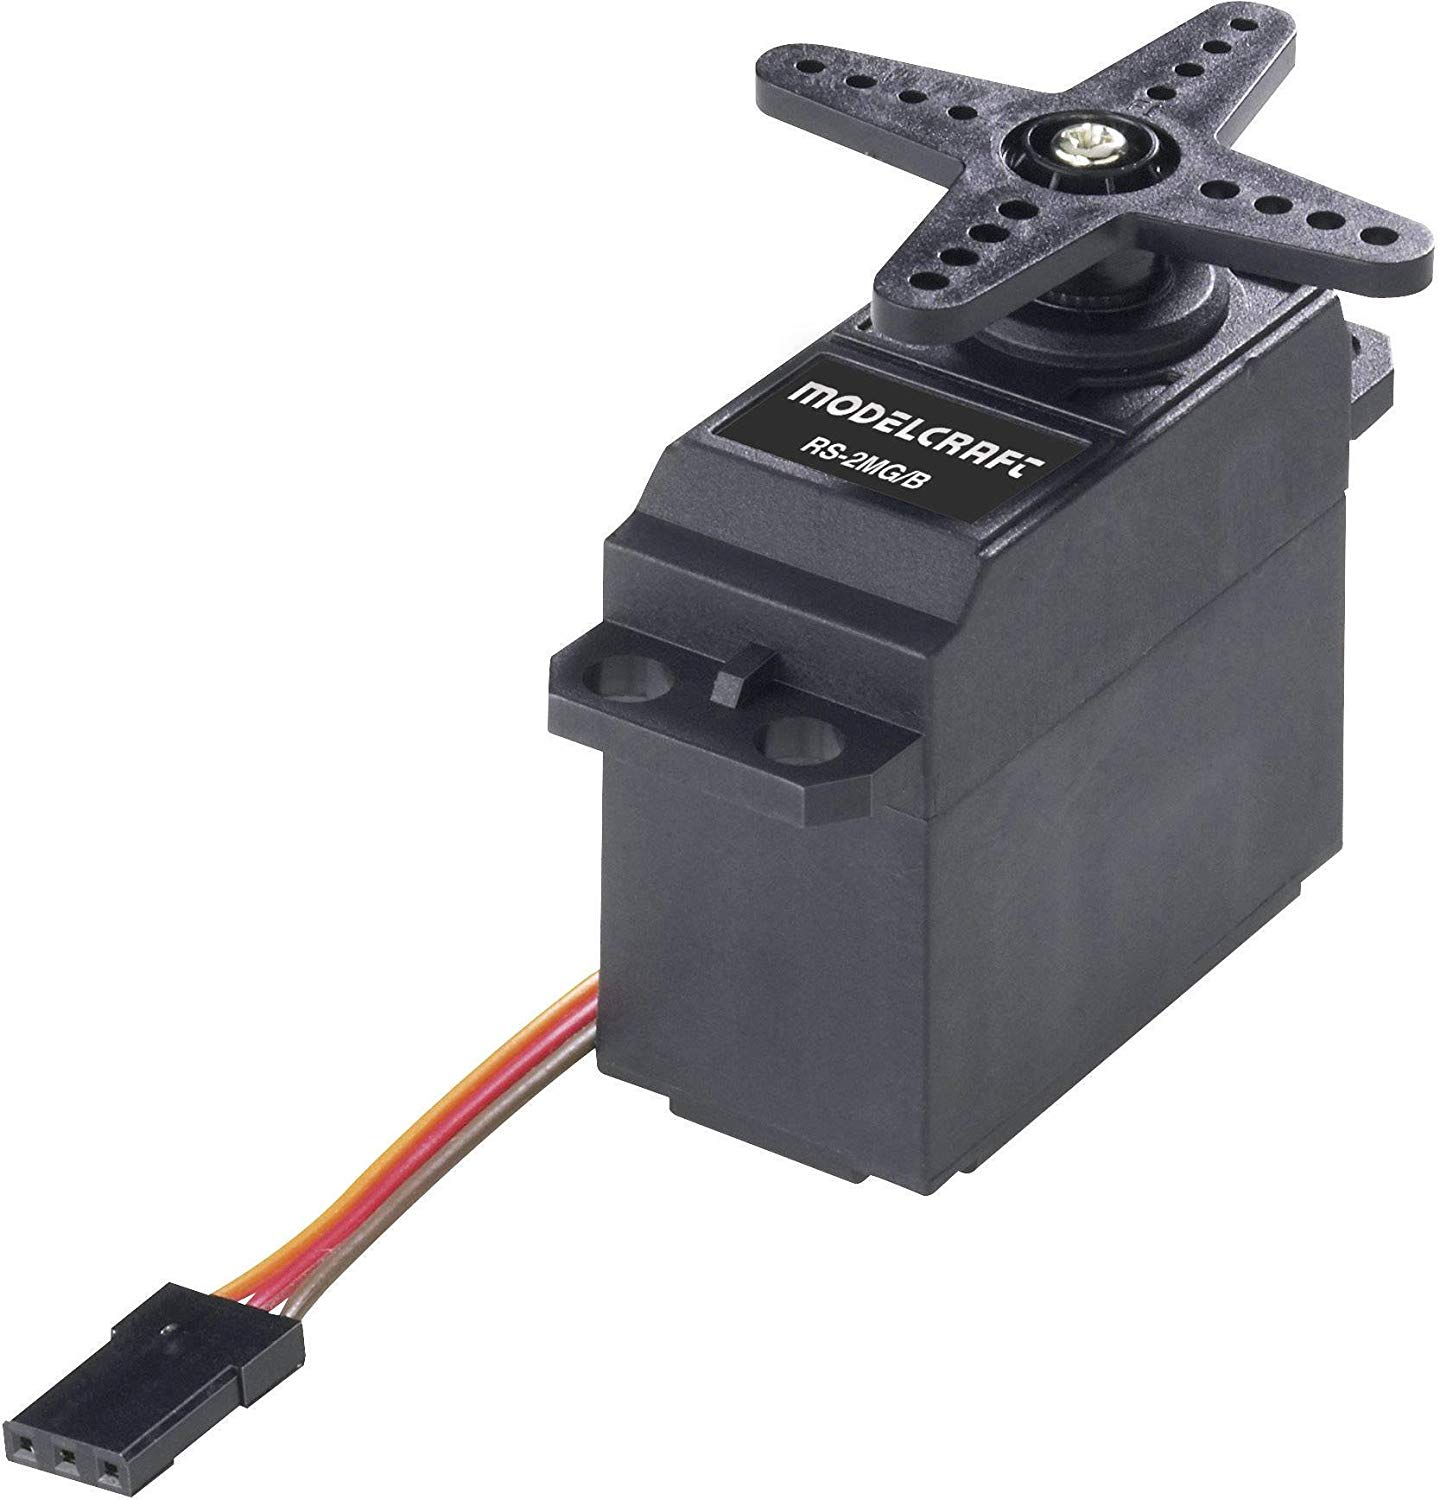
\includegraphics[scale=0.1]{imagenes/servo.jpg}
  \end{center}
  \caption{Imagen de un servomotor.}
  \label{figure:servomotor:}
\end{figure}

Un servomotor se compone de un motor, un circuito de control, un potenciómetro y un conjunto de engranajes. Los cuales se caracterizan por un consumo energético muy reducido.\\

Podemos definir un servomotor como un motor al que se le ha añadido un sistema de control, un potenciómetro y un conjunto de engranajes. Con anterioridad los servomotores no
permitían que el motor girara 360 grados, solo aproximadamente 180; sin embargo, hoy en día existen servomotores en los que puede ser controlada
su posición y velocidad en los 360 grados. Los servomotores son comúnmente usados en modelismo para controlar y dotar de movimiento multitud de elementos.\\

En cuanto al conexionado, los servomotores poseen tres cables de conexión externa, alimentación, tierra y control. Mediante éste último indicamos el ángulo al cuál queremos llegar. 
Un servomotor normal tiene un movimiento angular de 0 a 180º, caso del utilizado en este proyecto. El ángulo está determinado por la duración de un pulso. El servomotor 
espera ver un pulso cada 20 milisegundos. La longitud del pulso determinará el giro que ha de realizar el motor. Un pulso de 1.5 ms hará que el motor se posicione en la posición 
neutra, a 90º respecto al eje. En caso contrario, si el pulso es menor de 1.5 ms,  el motor se acercará a 0º, y si el pulso es mayor de 1.5ms, el eje se acercará a los 180 grados.\\

Inicialmente se pensó en utilizar un dispositivo de este tipo para el control de la dirección del vehículo pero debido a que el chasis utilizado ya incorporaba un motor de continua tradicional
que cumplía muy bien su cometido, éste ha sido descartado. Dicho servomotor podría ser utilizado para dotar de movimiento de elevación, por ejemplo a la cámara que incorpora el vehículo. Tal y como
se recoge en la sección \ref{sec:mejoras_futuras} correspondiente a mejoras futuras.\\

\subsection{Interconexión de elementos}

En el presente punto se recogen todos aquellos puntos de interés referentes a la interconexión de elementos utilizados, los cuales quedaron descritos en la sección \emph{Tecnologías hardware}
\ref{sec:tecnologias-hardware} junto con sus especificaciones.\\

Comenzando por el módulo central del sistema, la placa Raspberry Pi Model B+\footnote{ Todo lo referente a la utilización de los puertos de Entrada/Salida, puesta en funcionamiento y
utilización de la placa Raspberry Pi se encuentra disponible en el manual de usuario \cite{book:Raspberry} elaborado por uno sus creadores. }, dispone de una serie de pines denominados GPIO (General Purpose Input/Output) es, como su propio nombre indica, 
un sistema de E/S (Entrada/Salida) de propósito general, es decir, una serie de conexiones que se pueden usar como entradas o salidas para usos múltiples. Estos pines se encuentran en todos
los modelos de Raspberry Pi.\\

Comentar que debido a la incorporación de una placa Arduino no se han utilizado ninguno de los puertos GPIO que la Raspberry Pi ofrece a pesar de que hubiesen resultado perfectamente 
funcionales y encontrándose disponibles para cualquier ampliación que se desee realizar con posterioridad. Se ha optado por dejar a la placa tan solo como unidad central de 
procesamiento, conexión del vehículo con una red de internet y transmisión de los datos capturados al servidor y escucha de comandos recibidos.\\

Pero existe una problemática y es que no podemos conectar directamente los pines de salida de nuestra placa Arduino directamente a los motores. Esto es debido a
que la placa no dispone de potencia suficiente para mover actuadores. De hecho, la función de la placa no debe ser ejecutar acciones sino mandar ejecutar acciones a drivers que
realicen el trabajo pesado.\\

\subsection{Driver motores}
\label{sec:drivers}

Un driver motor es un dispositivo, o grupo de dispositivos, que se utilizan para controlar de una manera predeterminada el funcionamiento de un motor eléctrico. El control 
se consigue mediante unas señales de entrada, ya sean analógicas o bien digitales, con las que 
conseguimos:

\begin{itemize}
 \item Seleccionar el sentido de giro del motor: gracias a la utilización de un driver, podemos 
elegir el sentido horario o anti horario del motor de manera muy simple.
\item Regular la velocidad mediante el uso de una señal PWM, el driver permitirá regular la velocidad de variación de un motor DC
\item Permite la alimentación necesaria para el correcto funcionamiento del motor.
\item Protección del circuito: al incluir un driver en el circuito, nos ofrece protección contra 
posibles sobrecargas y fallas que puedan aparecer.
\end{itemize}

Para ello empleamos el L298N, un controlador (driver) de motores integrado en un módulo, el cual nos permite encender y controlar dos motores de corriente continua desde una Raspberry Pi, Arduino o
cualquier placa similar, variando tanto la dirección como la velocidad de giro.\\

La corriente máxima que el L298N es capaz de suministrar a los motores es, en teoría, 2A por salida, permitiendo alcanzar hasta los 3A de pico, y una tensión de alimentación de 3V
a 35V. Sin embargo, el L298N tiene una eficiencia energética extremadamente baja. La electrónica supone una caída de tensión de unos 3V, es decir, la tensión que recibe el motor
es unos 3V inferior a la tensión de alimentación, todo ello unido a la gran cantidad de calor que disipa el driver.\\

Estas pérdidas se traducen en que, a efectos prácticos, es difícil que podamos obtener más de 0.8-1A por fase sin exceder el rango de temperatura de funcionamiento.\\

El L298N tiene la ventaja de que incorpora protecciones contra efectos que pueden producirse al manejar motores de corriente continua. Dispone de protecciones contra situaciones
de elevada intensidad, temperatura, y diodos de protección contra polaridades incorrectas.\\

Dicho módulo cuenta con todos los componentes necesarios para funcionar sin necesidad de elementos adicionales entre los que incluye un regulador \textbf{LM7805} que suministra 5V
a la parte lógica del integrado L298N. Además cuenta con jumpers de selección para habilitar cada una de las salidas del módulo (A y B). La \textbf{salida A} esta conformada
por \textbf{OUT1} y \textbf{OUT2} y la \textbf{salida B} por \textbf{OUT3} y \textbf{OUT4}. Los pines de habilitación 
son \textbf{ENA} y \textbf{ENB} respectivamente.\\

Los pines \textbf{IN1}, \textbf{IN2}, \textbf{IN3} y \textbf{IN4}; son los pines de entrada donde se conectan a pines digitales de Arduino para poder controlar el motor.\\

La alimentación del driver es variable existiendo dos modos de funcionamiento, ya que dispone de un regulador de tensión de 5v incorporado. Cuando el jumper de selección de 5V se
encuentra activo, el módulo permite una alimentación de entre 6V a 12V DC. Como el regulador se encuentra activo, el pin marcado como +5V tendrá un voltaje de 5V DC.
Este voltaje se puede usar para alimentar la parte de control del driver ya sea un micro-controlador o un Arduino no debiendo superar los 500 mA.\\

Cuando el jumper de selección de 5V se encuentra inactivo, el driver permite una alimentación de entre 12V a 35V DC. Como el regulador no está funcionando, tendremos que conectar el pin de +5V a una tensión de 5V para alimentar la parte 
lógica del L298N.\\

En  este  caso  se  utilizará una fuente de 11,1V manteniendo el jumper activo, y así alimentar la parte de control del driver.\\

En la figura \ref{diagrama:L298N-salidas} se muestra el módulo empleado con sus diferentes pines al detalle.\\

\begin{figure}[H]
  \begin{center}
    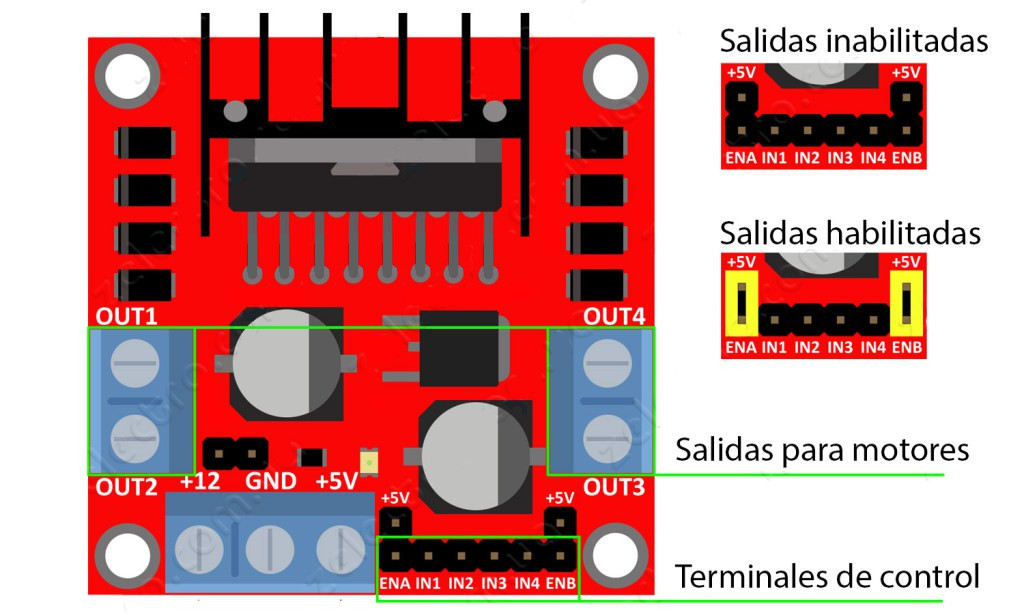
\includegraphics[scale=2]{imagenes/L298N-conexiones.jpg}
  \end{center}
  \caption{Pines de entrada/salida del módulo L298N empleado.}
  \label{diagrama:L298N-salidas}
\end{figure}

Centrándonos a un nivel más bajo, dicho módulo incorpora, lo que conocemos en electrónica como puente en H, el cual es un circuito electrónico que permite cambiar el sentido de giro de los 
motores de corriente continua. Este circuito lo componen cuatro interruptores, los cuales pueden ser mecánico o electrónicos (diodos, transistores...) de forma que,
en función de cuales se abran o cierren, permitirán cambiar el sentido de alimentación de un motor.  Los podemos encontrar como circuitos integrados, pero también se
pueden crear con componentes discretos.\\

\begin{figure}[H]
  \begin{center}
    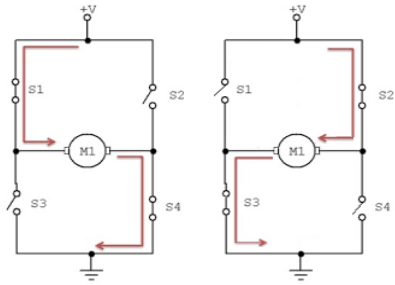
\includegraphics[scale=0.7]{imagenes/esquema_puente_h.png}
  \end{center}
  \caption{Diagrama de funcionamiento del puente H.}
  \label{esquema:funcionamiento_puente_h}
\end{figure}

El funcionamiento de un puente H es bastante simple. Siguiendo la Figura \ref{esquema:funcionamiento_puente_h} podemos observar que, cuando se cierran los interruptores \textbf{S1} y \textbf{S4}, y se abren \textbf{S2} y \textbf{S3}, se aplica una tensión positiva en bornes del motor, así 
que este gira en un sentido y cuando se abren los interruptores \textbf{S1} y \textbf{S4} y se cierran \textbf{S2} y \textbf{S3}, se invierte la tensión en bornes del motor, haciendo que el motor gire en sentido contrario.\\

Y, por contra, si todos los interruptores están abiertos el motor no girará. \\

Para el caso del proyecto, hemos empleado utilizado las salidas para la conexión de dos motores, empleando así todas las que el driver proporciona. Una de ellas para traccionar
el vehículo y la segunda para el accionamiento de la dirección.\\

Se ha optado finalmente por emplear un motor DC para la dirección debido que el chasis empleado para la construcción del robot ya lo traía así incorporado y se ha decidido reutilizar.
De igual modo se podría haber empleado un servomotor para el accionamiento de la dirección, pero debido a una mayor simplicidad en el montaje y puesto que el motor ya incorporado
dispone de una mejor sujeción al chasis así se ha decidido.\\

\subsection{Motores}

En la figura \ref{img:sistema_direccion} se muestra el motor de dirección empleado junto con el sistema de topes de recorrido que incorpora.\\


\begin{figure}[H]
  \begin{center}
    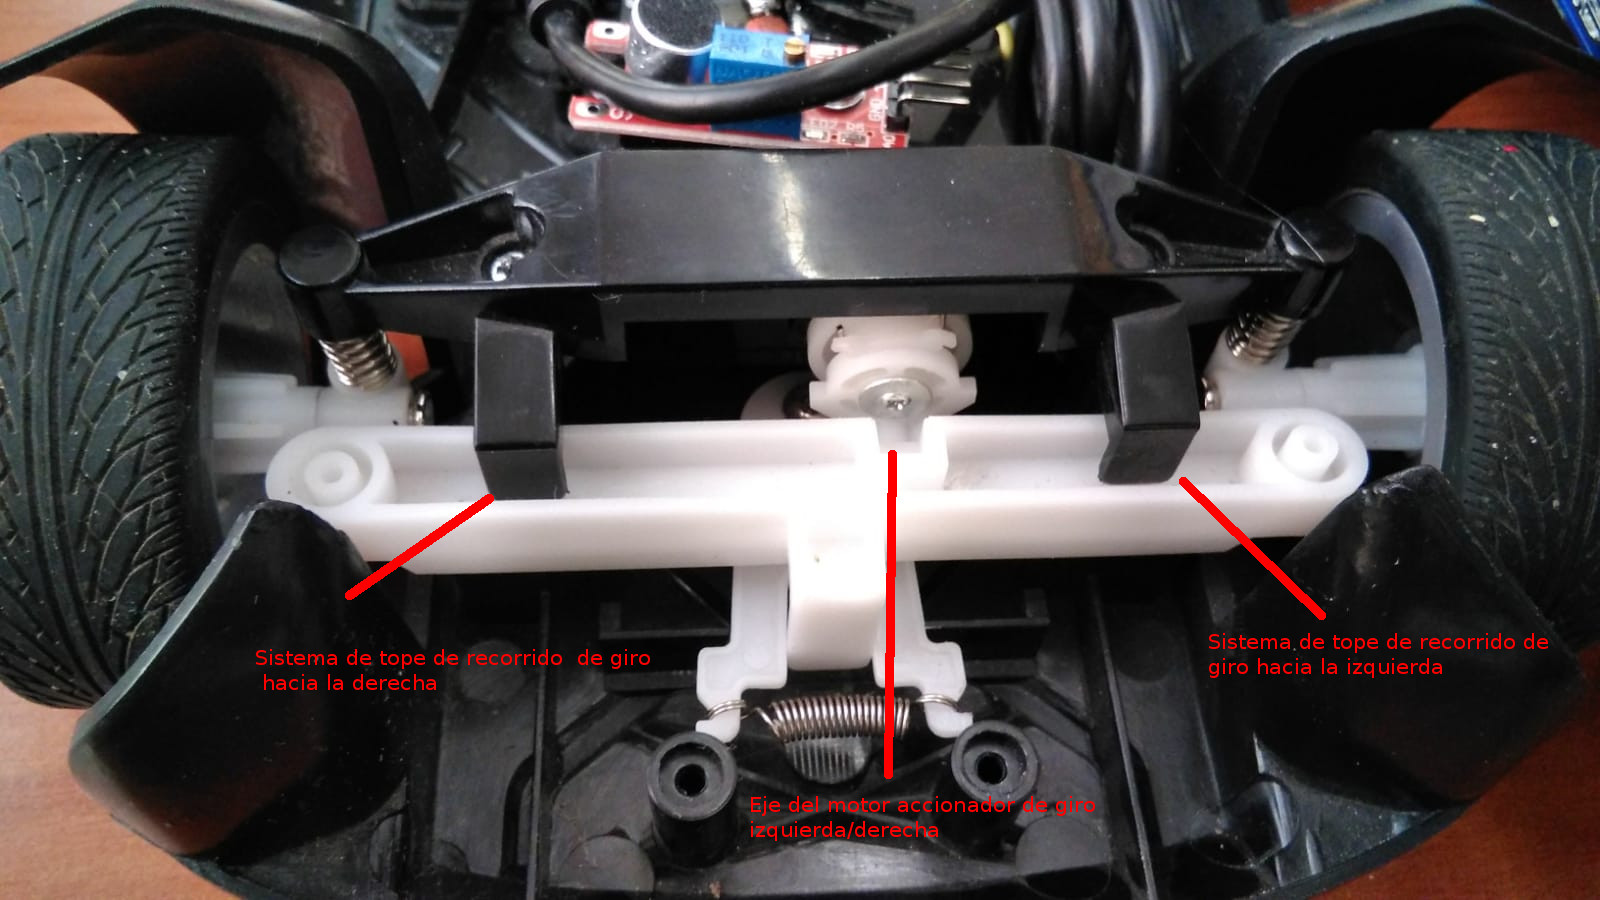
\includegraphics[scale=0.2]{imagenes/robot/motor-direccion.jpg}
  \end{center}
  \caption{Sistema de accionamiento de la dirección.}
  \label{img:sistema_direccion}
\end{figure}

Motor de tracción del vehículo situado en su parte trasera, figura \ref{img:motor_traccion}.

\begin{figure}[H]
  \begin{center}
    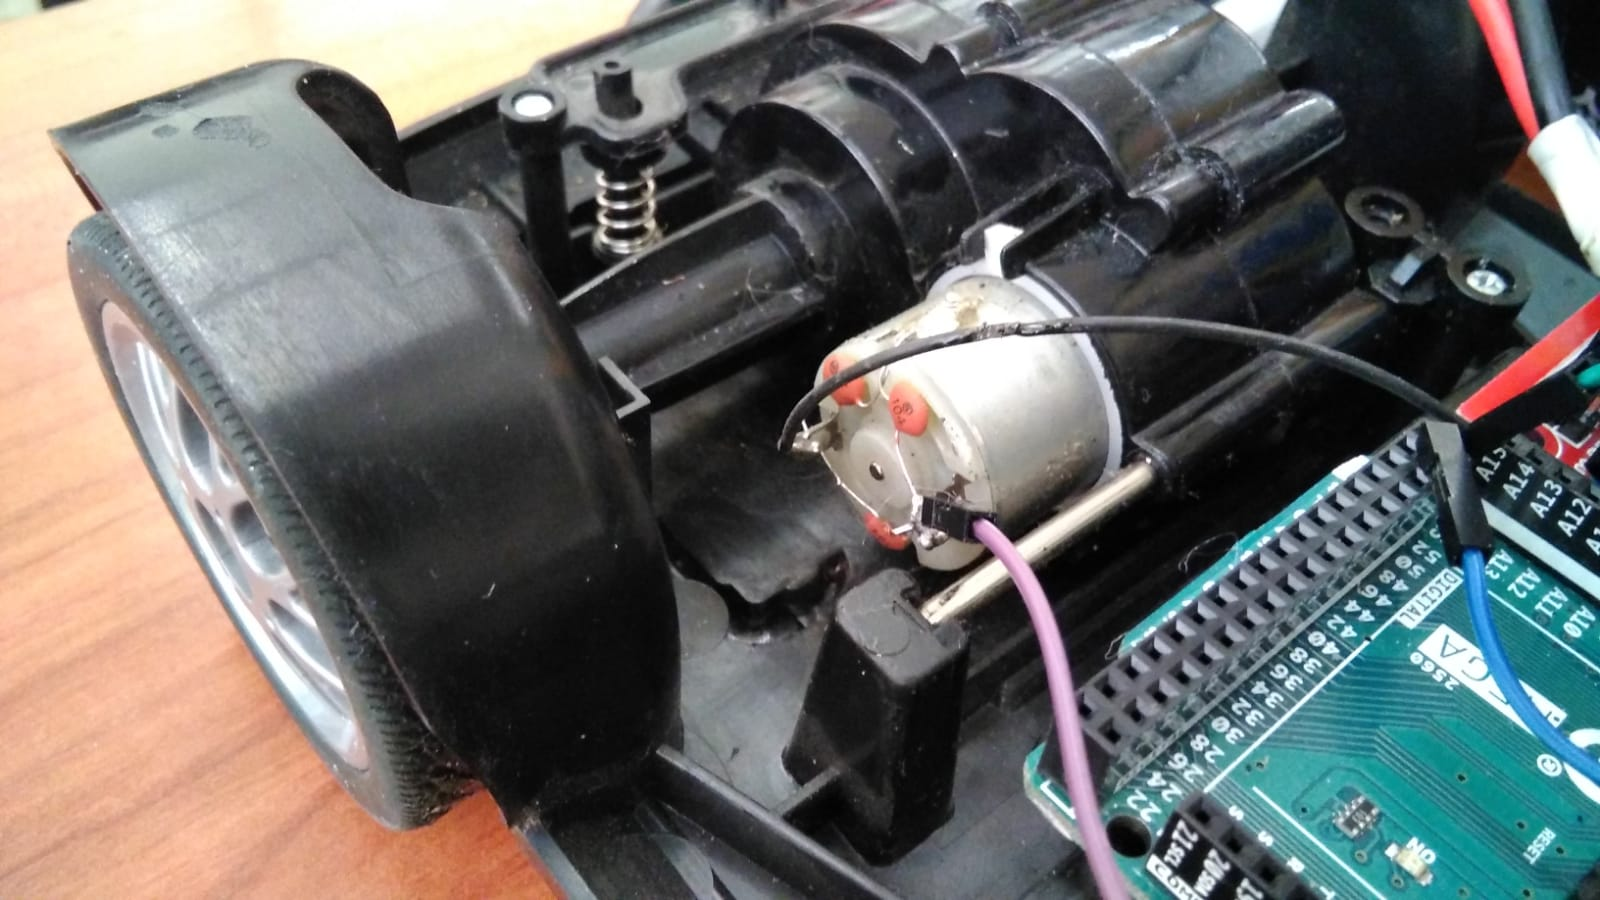
\includegraphics[scale=0.2]{imagenes/robot/motor-traccion.jpeg}
  \end{center}
  \caption{Vista del motor de tracción.}
  \label{img:motor_traccion}
\end{figure}


\section{Alimentación}
\label{sub:alimentación}

Resulta de vital importancia el dotar de energía nuestro proyecto siendo una de las partes más importantes y críticas del mismo. La selección de los componentes adecuados
requiere una realización previa de estudio de las necesidades que se desean cubrir puesto que una decisión equivocada puede implicar un defectuoso
comportamiento del conjunto.\\

Por tanto, cuando se escoja la batería se deben tener en cuenta los siguientes puntos:\\

\begin{enumerate}

 \item \textbf{Consumo máximo del robot:} A partir de las características de todos los
componentes, se tiene que mirar cuál será su consumo máximo (motores a pleno
rendimiento, electrónica consumiendo al máximo, etc.), y una vez determinado,
buscar una fuente de alimentación que sea capaz de proporcionar esta corriente.

\item \textbf{Pico de consumo máximo:} Cuando un motor se pone en marcha, se origina un
pico de consumo por la resistencia que tiene a moverse. Este pico será mayor
cuanta más velocidad se da y/o mayor carga se desee mover. La batería debe ser
capaz de proporcionar estos picos y no ver comprometido su funcionamiento. Si no
fuera capaz, provocaría una bajada de tensión para proporcionar esta corriente, y
podría apagar el resto de la electrónica. Este valor se suele encontrar en las
baterías como C. Por ejemplo, si la batería es de 1000 mAh con un C de 10, podrá
suministrar picos de hasta 10000 mA, o lo que es lo mismo, 10 Amperios.


\item \textbf{Capacidad:} Todas las baterías recargables dan una cifra de carga, se suele
expresar en Ah (Amperios/hora) o mAh (miliamperios/hora). Esta cifra indica
cuantos amperios/hora es capaz de dar la batería antes de descargarse. Por tanto,
si el consumo es de 10 mA y la batería es de 100 mAh, el equipo podrá estar en
marcha durante 10 horas, si por el contrario el consumo es de 100mA y la batería
es de 10mAh, el equipo solo podrá estar en funcionamiento 6 minutos.

\item \textbf{Voltaje:} Este valor dependerá de las tensiones que se necesiten en el circuito, ya
sea por parte del motor, o por parte de la electrónica de control.

\end{enumerate}

En ocasiones, muchos de los diseños de los robots se realizan incorporando dos baterías separadas. Utilizando esta configuración separamos la
parte digital (sistema de control y sensado) de la parte analógica (motores). Los motores son muy ruidosos, y a través de la alimentación pueden inducir ruidos
al resto de circuitería. En el mejor de los casos el sistema será lo suficientemente robusto para soportar estos problemas, pero muchas
veces este ruido falsea las medidas, o hasta puede provocar que la parte del control se resetee.\\

Por esta razón, se ha optado por el uso de dos baterías para la alimentación del conjunto. Una para dotar de energía a la placa de control y otra para la alimentación de los 
motores debido a la gran cantidad de energía que éstos demandan y su elevado consumo.\\

Para la alimentación de la placa Raspberry Pi, se ha optado por la utilización de una batería de Litio desarrollada específicamente para su uso con este modelo de placas el cual permite una integración
perfecta. Dicho módulo de alimentación queda descrito en la subapartado correspondiente de herramientas utilizadas \ref{componente:bateria-expansion}.\\

Imagen de la Raspberry Pi junto con su módulo de expansión de batería:

\begin{figure}[H]
  \begin{center}
    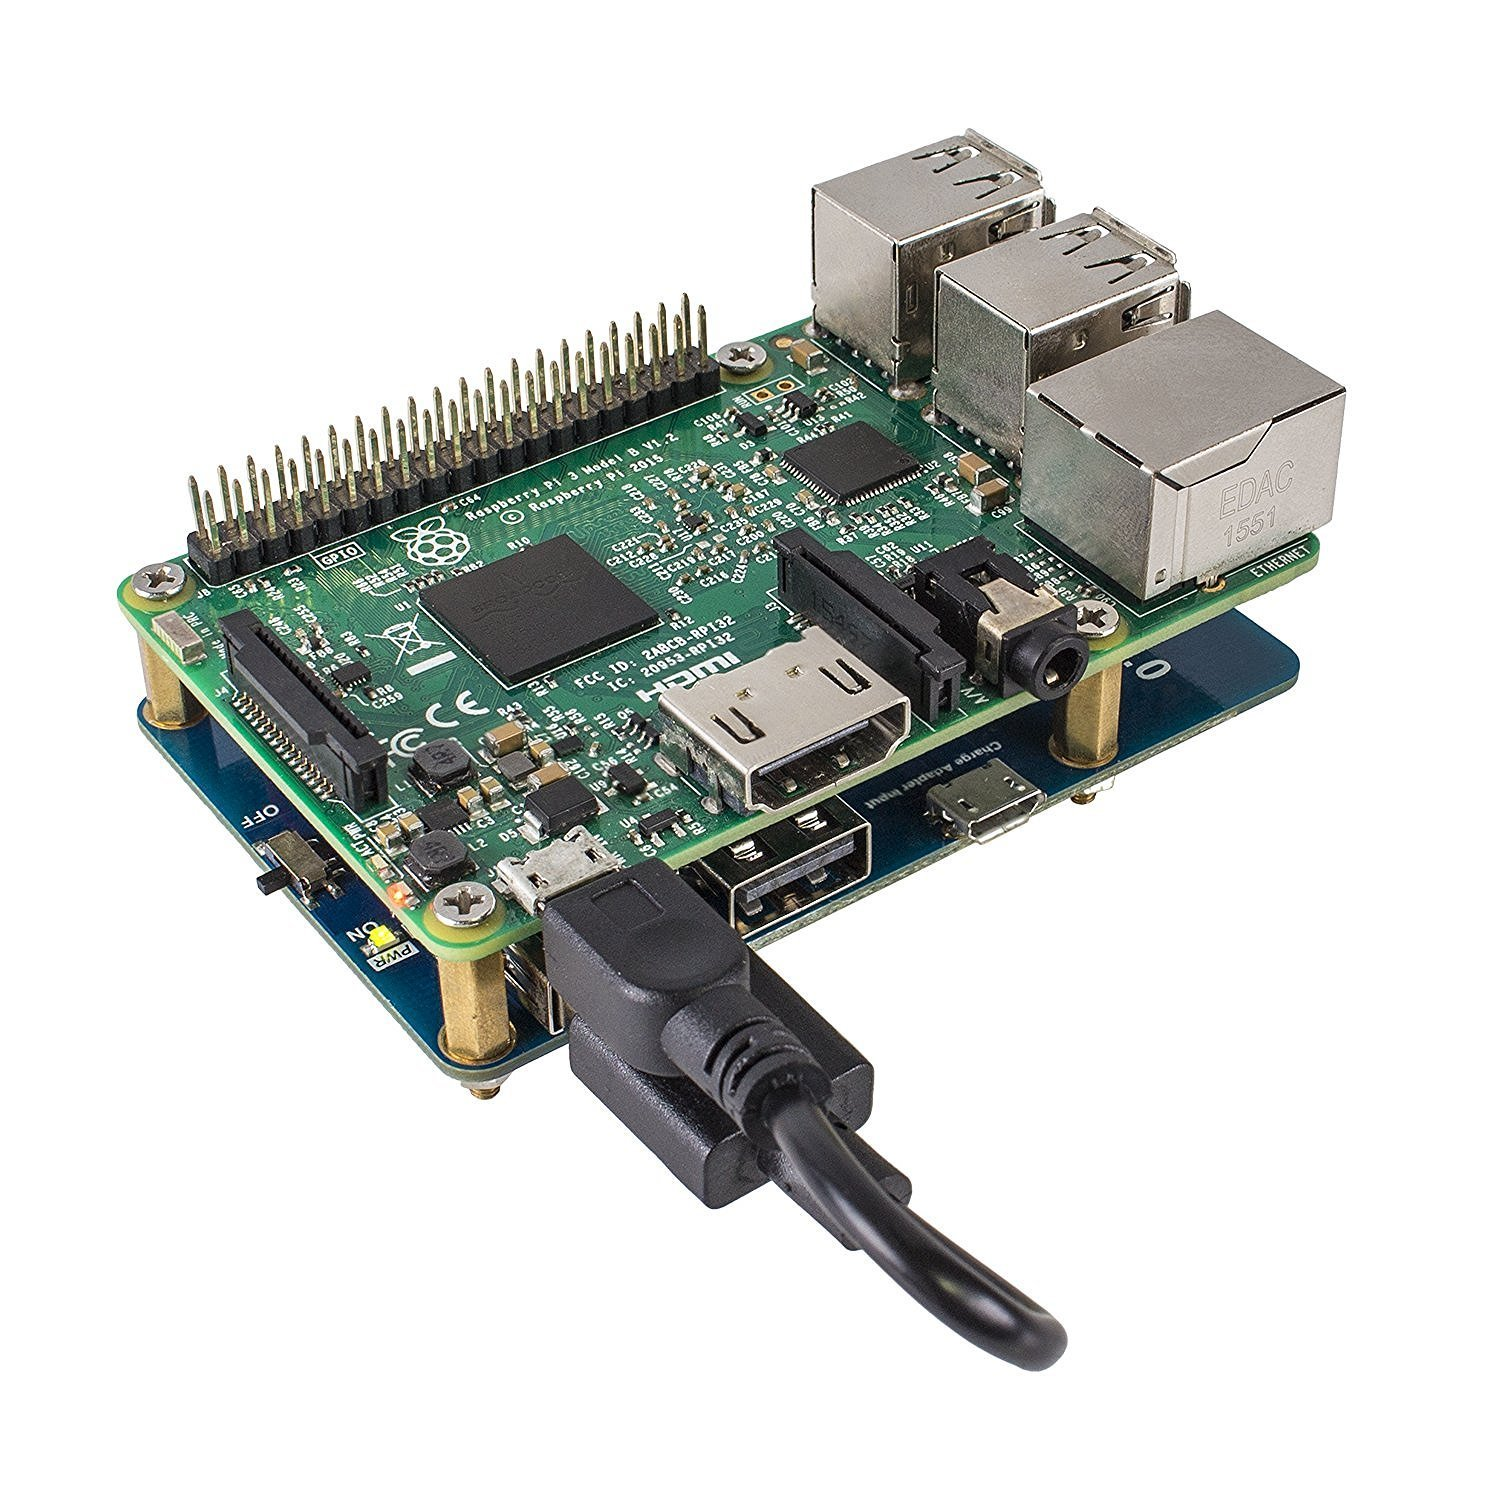
\includegraphics[scale=0.15]{imagenes/modulo-expansion-rpi.jpg}
  \end{center}
  \caption{Conjunto Raspberry Pi y módulo de expansión de alimentación.}
  \label{figura:rpi-modulo-bateria}
\end{figure}

Imagen de la batería LiPo para la alimentación de los motores:

\begin{figure}[H]
  \begin{center}
    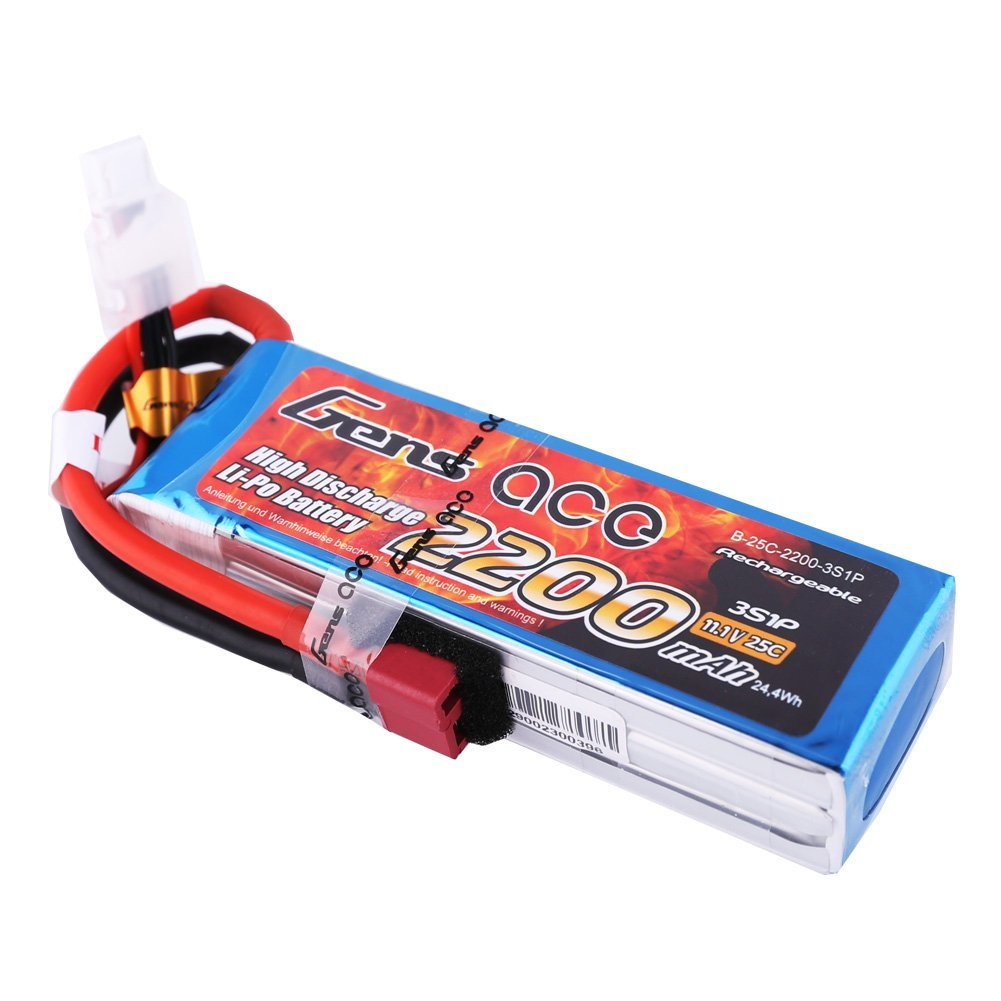
\includegraphics[scale=0.2]{imagenes/robot/bateria.jpg}
  \end{center}
  \caption{Batería LiPo que alimenta los motores.}
  \label{figura:rpi-modulo-bateria}
\end{figure}


\subsubsection{ Alimentación USB/Protoboard }

Para alimentar la protoboard sin tener que modificar un cable USB, se ha decidido utilizar una pequeña tarjeta que se conecta en los carriles de tensión de la tarjeta Protoboard, y
proporciona los 5 V de entrada del USB (o de un conector Jack) a las líneas de alimentación de la protoboard. Además este dispositivo integra un interruptor, que permitirá activar y
desactivar los motores, y puede regular la tensión a 3,3 Voltios.\\

\begin{figure}[H]
  \begin{center}
    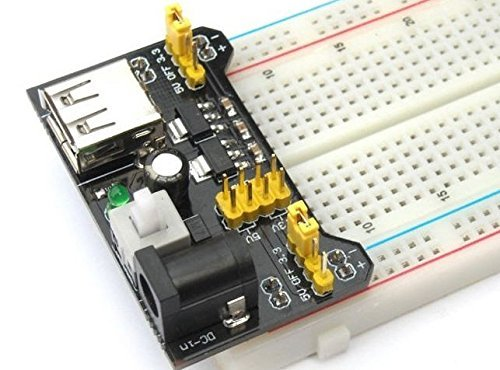
\includegraphics[scale=0.3]{imagenes/alimentador_usb_protoboard.jpg}
  \end{center}
  \caption{Adaptador de entrada USB a protoboard.}
  \label{figura:alimentador_usb_protoboard}
\end{figure}

La alimentación de este módulo se puede realizar de dos formas: mediante el uso de una pila o batería, o mediante un cable USB. Para saber que está correctamente alimentado, este 
dispositivo incorpora un indicador led que avisará si se está usando de forma correcta. Otra característica importante de este módulo, es la posibilidad de elegir la tensión de
salida que proporciona, pudiendo seleccionar una alimentación de 5V y otra de 3,3V a la vez.\\

En la Figura \ref{figura:alimentador_usb_protoboard_esquema} puede verse el esquema eléctrico del módulo.\\

\begin{figure}[H]
  \begin{center}
    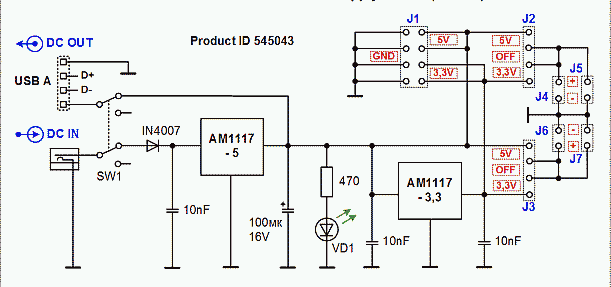
\includegraphics[scale=0.5]{imagenes/esquema_alimentador_protoboard.png}
  \end{center}
  \caption{Adaptador de entrada USB a protoboard.}
  \label{figura:alimentador_usb_protoboard_esquema}
\end{figure}

Siguiento el esquema \ref{figura:alimentador_usb_protoboard_esquema} Podemos diferenciar los distintos componentes según su funcionalidad dentro del módulo:

\begin{itemize}
 \item \textbf{Alimentación USB:} Esta entrada solo se utiliza para la alimentación de 5 voltios mediante un conector USB hembra.
 Los pines centrales, D+ y D- no están conectados a ningún elemento, por lo que no puede recibir datos.

 \item \textbf{Alimentación externa:} Se trata de un conector tipo Jack hembra al que se le puede colocar cualquier tipo de batería
 o pila que se encuentre entre los rangos de 6 y 12V permitidos por el módulo.
 
 \item \textbf{AM1117-5 y AM1117-3.3:} Son los dos reguladores de tensión que incorpora el módulo MB102 para regulación de tensión de salida hasta los valores 
 5 y 3,3V respectivamente.
 
 \item \textbf{ Diodos y condensadores} También incorpora una serie de diodos zener \footnote{El diodo Zener es un diodo de silicio fuertemente dopado​ que se ha construido para que funcione en las zonas de rupturas, recibe ese nombre por su inventor Clarence Melvin Zener. El diodo Zener es la parte esencial de los reguladores de tensión casi constantes con independencia de que se presenten grandes variaciones de la tensión de red, de la resistencia de carga y temperatura. } 
 de portección ante posibles inversiones de polaridad junto con un diodo led para comprobar el correcto funcionamiento del módulo.
 
 \item \textbf{SW1:} Botón cuya finalidad es encender o apagar el módulo de alimentación.
 
 \item \textbf{J1:} Serie de pines en los cuales se tiene una tensión de 5V y 3.3V para la conexión de los diferentes elementos. De los ocho pines que dispone, cuatro pines son
 de GND, dos pines son de 5V y los otros dos pines restantes son de 3.3V.
 
 \begin{figure}[H]
  \begin{center}
    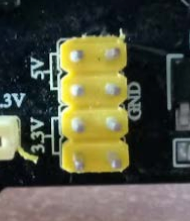
\includegraphics[scale=0.5]{imagenes/usb_board_pines.png}
  \end{center}
  \caption{Vista del conector J1.}
  \label{figura:conector_usb_board_j1}
\end{figure}

  \item \textbf{J2 y J3:} Pines para la selección de la tensión de salida del módulo. Para seleccionar la tensión debemos conectar un jumper\footnote{En electrónica y en particular en informática,
   un jumper o saltador es un elemento que permite cerrar el circuito eléctrico del que forma parte dos conexiones. Esto puede hacerse mediante soldadura (se derrite suficiente estaño para cerrar el circuito), soldando un cable o alambre entre ambos puntos o, lo más frecuente, conectado dos pines en hilera o paralelo mediante una pieza de plástico que protege el material conductor que cierra el circuito. Los más habituales tienen tamaños de 2,54 mm, 2 mm y 1,27 mm. } entre los pines en función de la
  tensión deseada.

   \begin{figure}[H]
  \begin{center}
    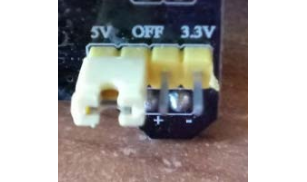
\includegraphics[scale=0.5]{imagenes/usb_board_vout.png}
  \end{center}
  \caption{Vista del conector J2 y J3.}
  \label{figura:conector_usb_board_vout}
\end{figure}

\item \textbf{J4 y J5:} Pines que incorpora el modulo en su parte inferior para la conexión de este en 
una protoboard.

   \begin{figure}[H]
  \begin{center}
    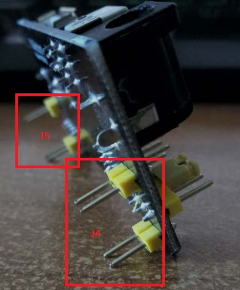
\includegraphics[scale=0.5]{imagenes/pin_usb_board.png}
  \end{center}
  \caption{Vista del conector J4 y J5.}
  \label{figura:conector_usb_board}
\end{figure}
  
\end{itemize}


\subsection{Interconexión entre módulos y fijación}

La conexión entre los diferentes módulos se realiza utilizando cables USB, y cables de interconexión entre la Raspberry/Arduino con la protoboard utilizándose la técnica
conocida como Wire-Wrap o cables tipo jumper-wire.\\

\begin{figure}[H]
  \begin{center}
    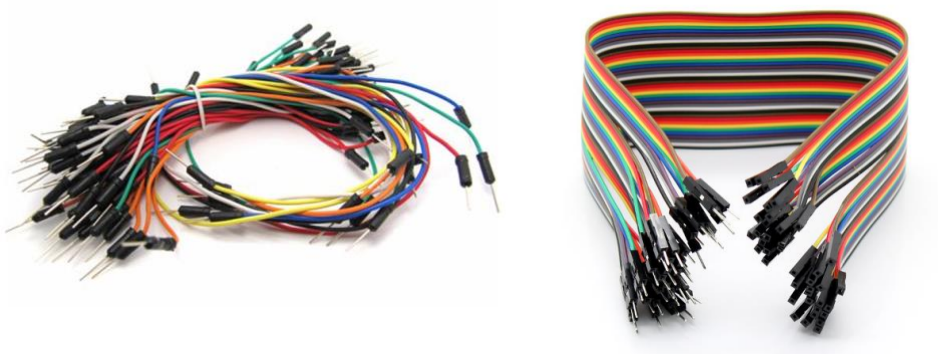
\includegraphics[scale=0.3]{imagenes/cables_interconexion.png}
  \end{center}
  \caption{Cables de interconexión para protoboard.}
  \label{figura:cables_interconexion}
\end{figure}

Para la fijación de los diferentes módulos al chasis se ha empleado tornillería y bridas, éstas últimas para mantener el cableado más ordenado.\\

\subsection{Conexionado general}

La siguiente imagen \ref{vista-conexiones} muestra una visión general de la disposición de todos los elementos que conforman el vehículo junto con sus conexiones:\\


\begin{figure}[H]
  \begin{center}
   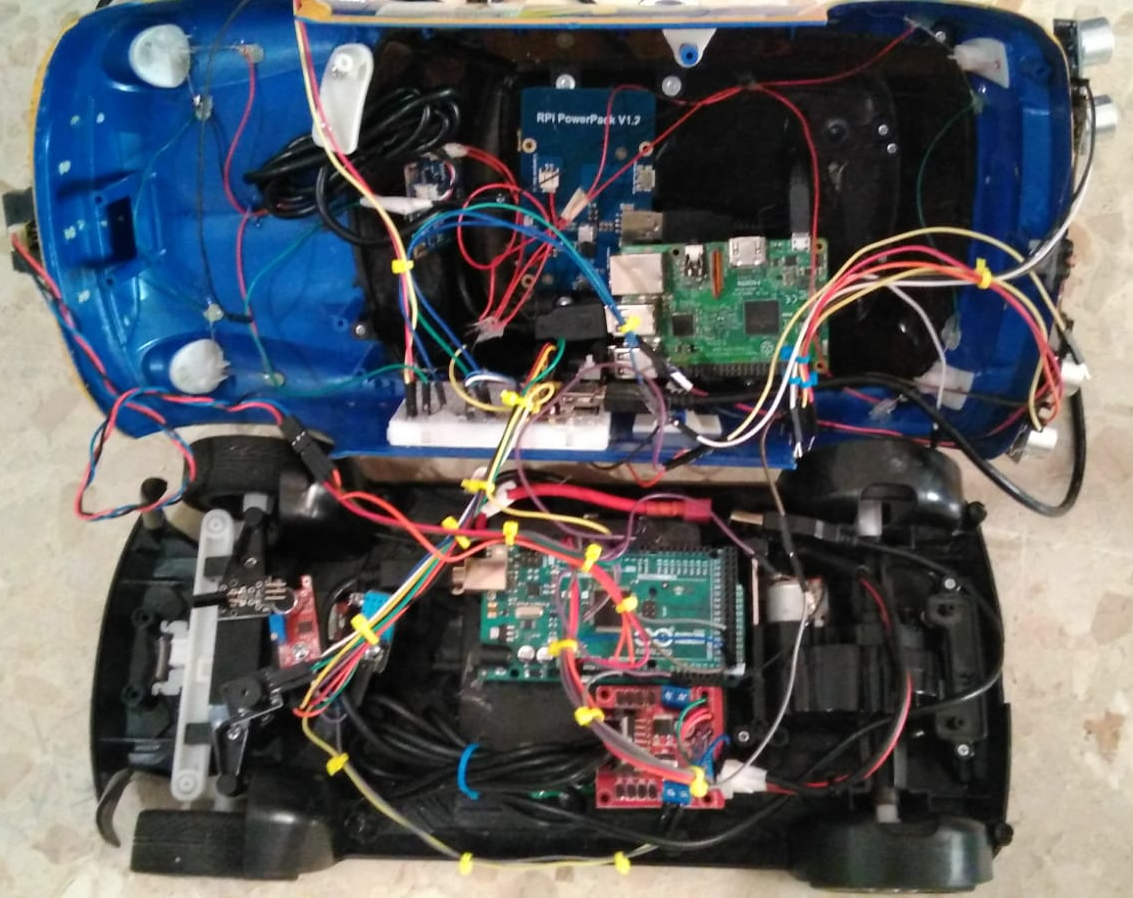
\includegraphics[scale=0.4]{imagenes/robot/general.png}
  \end{center}
  \caption{Vista del conexionado general del robot.}
  \label{vista-conexiones}
\end{figure}



\section{Iluminación}


\subsection{Leds}

Con el fin de dotar de iluminación al vehículo, se ha incorporado una serie de leds en los faros del vehículo tanto en su parte delantera como trasera. Dichos leds van concetados
a un pin del Arduino con la finalidad de poder encenderlos o apagarlos al deseo del operador. \\

La alimentación se encuentra conectada a un pin digital del arduino mientras que la masa a una entrada GND del mismo.\\

A continuación se muestra una imagen de los faros del vehículo en funcionamiento.\\


\begin{figure}[H]
    \centering
    \begin{subfigure}[b]{0.4\textwidth}
        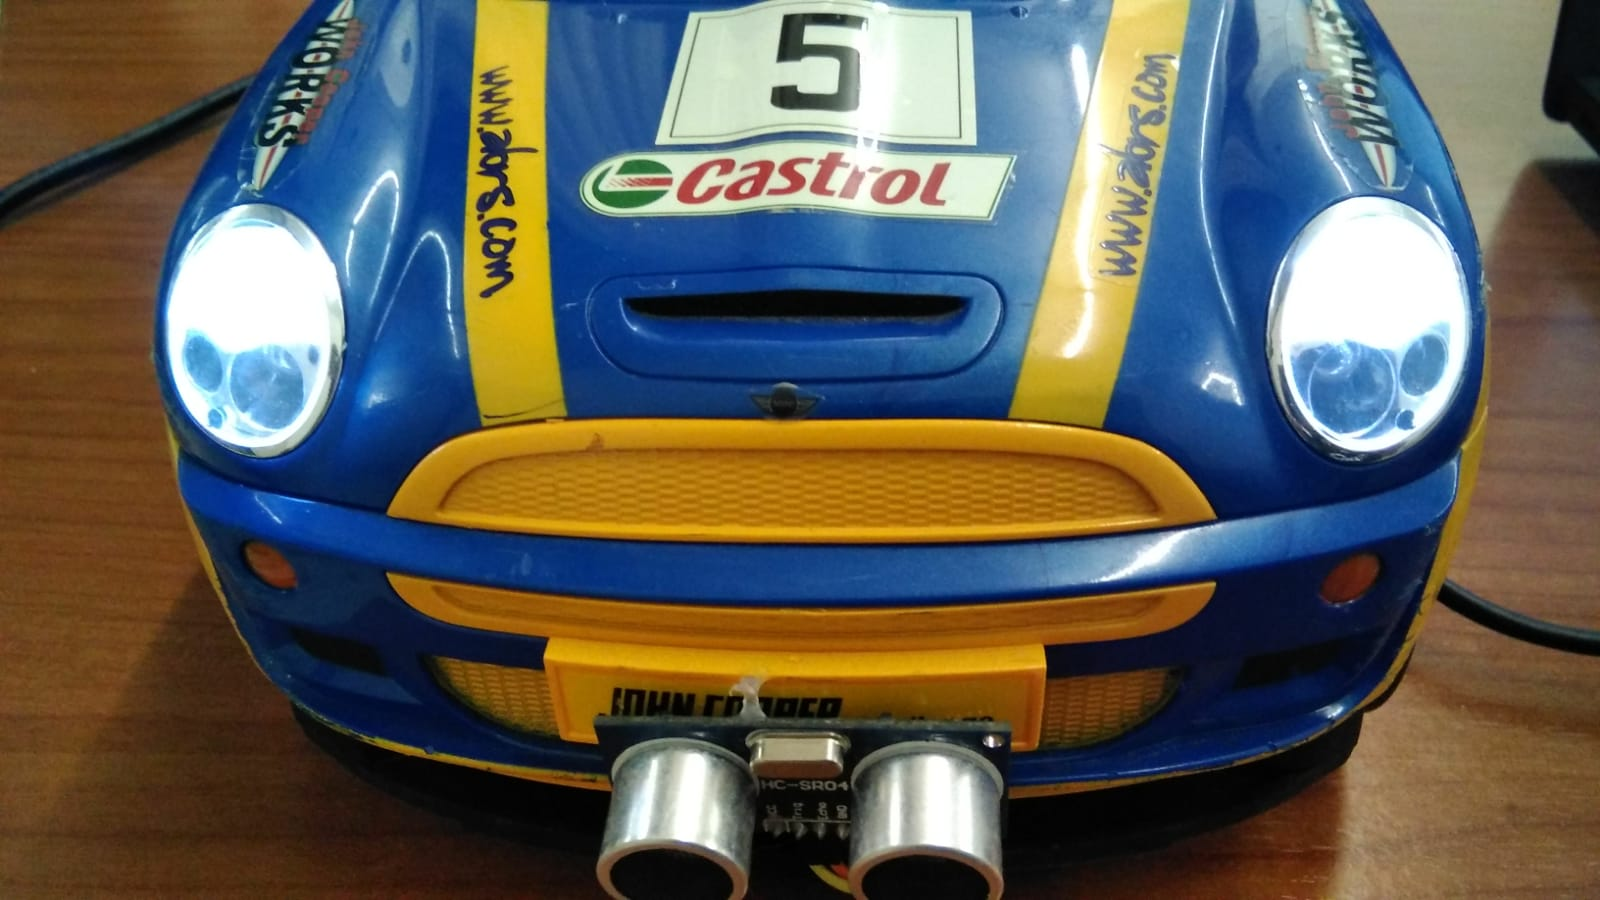
\includegraphics[width=\textwidth]{imagenes/robot/luces_delanteras.jpg}
        \caption{Iluminación frontal}
        \label{fig:gull}
    \end{subfigure}
    ~ %add desired spacing between images, e. g. ~, \quad, \qquad, \hfill etc. 
      %(or a blank line to force the subfigure onto a new line)
    \begin{subfigure}[b]{0.4\textwidth}
        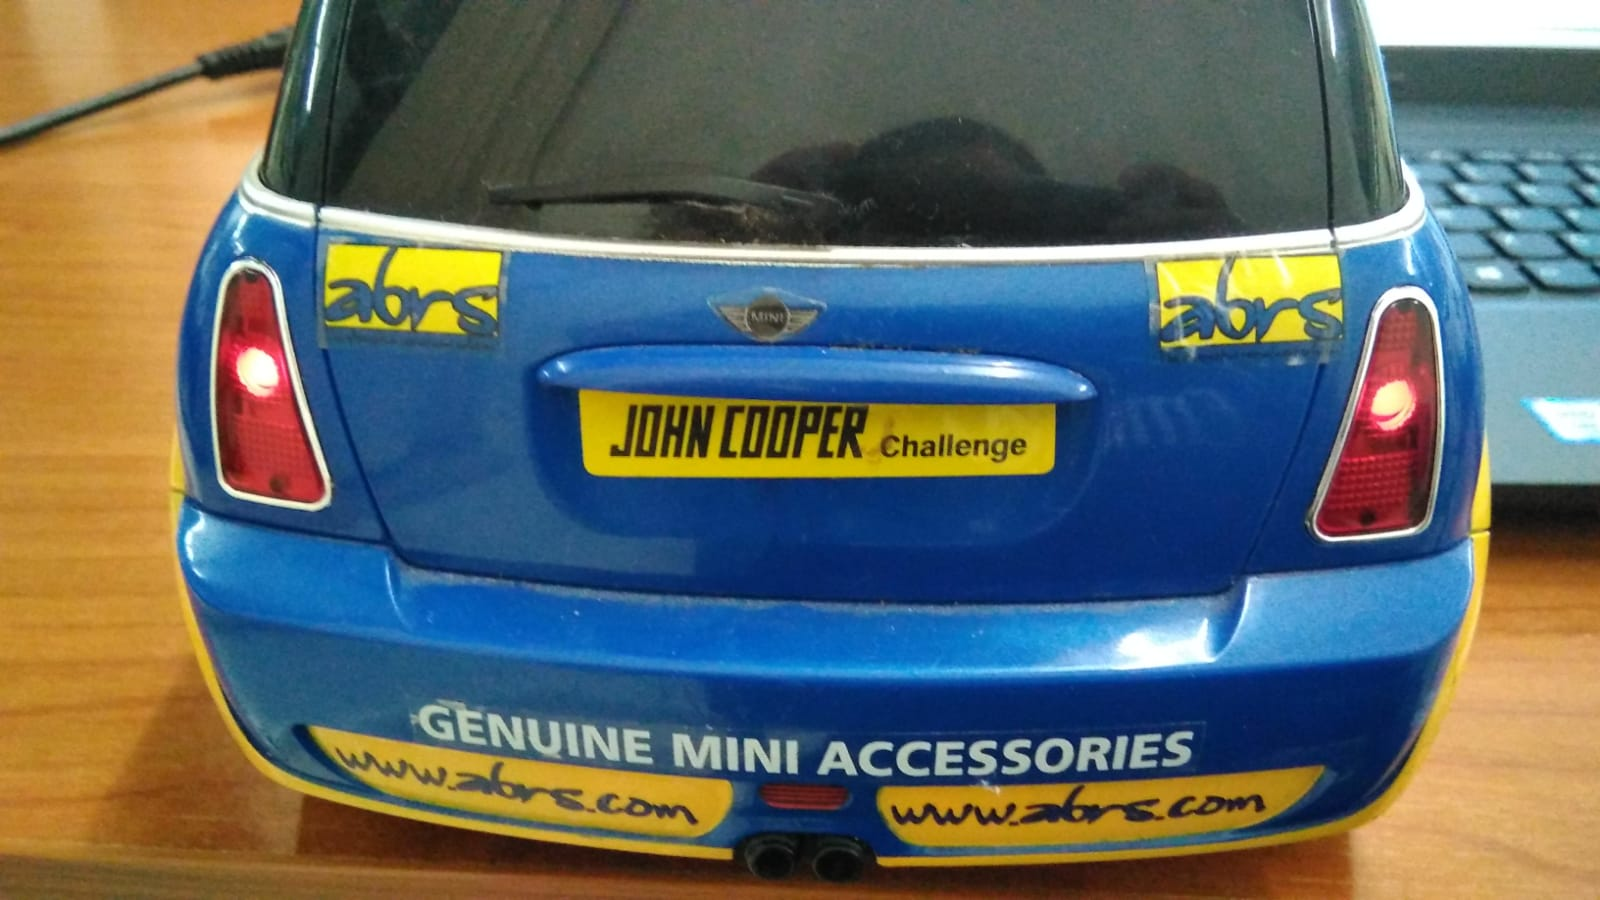
\includegraphics[width=\textwidth]{imagenes/robot/luces_traseras.jpeg}
        \caption{Iluminación trasera}
        \label{fig:tiger}
    \end{subfigure}
    \caption{Vehículo SensorRS con la iluminación activada.}\label{fig:iluminacion}
\end{figure}


Por otra parte, se ha incorporado un sensor detector de luminosidad para el encendido automático de luces en lugares de baja iluminación.\\


\subsubsection{Conexionado}

Representación del conexionado de los leds, figura \ref{img:leds_conexiones}.\\

\begin{figure}[H]
  \begin{center}
   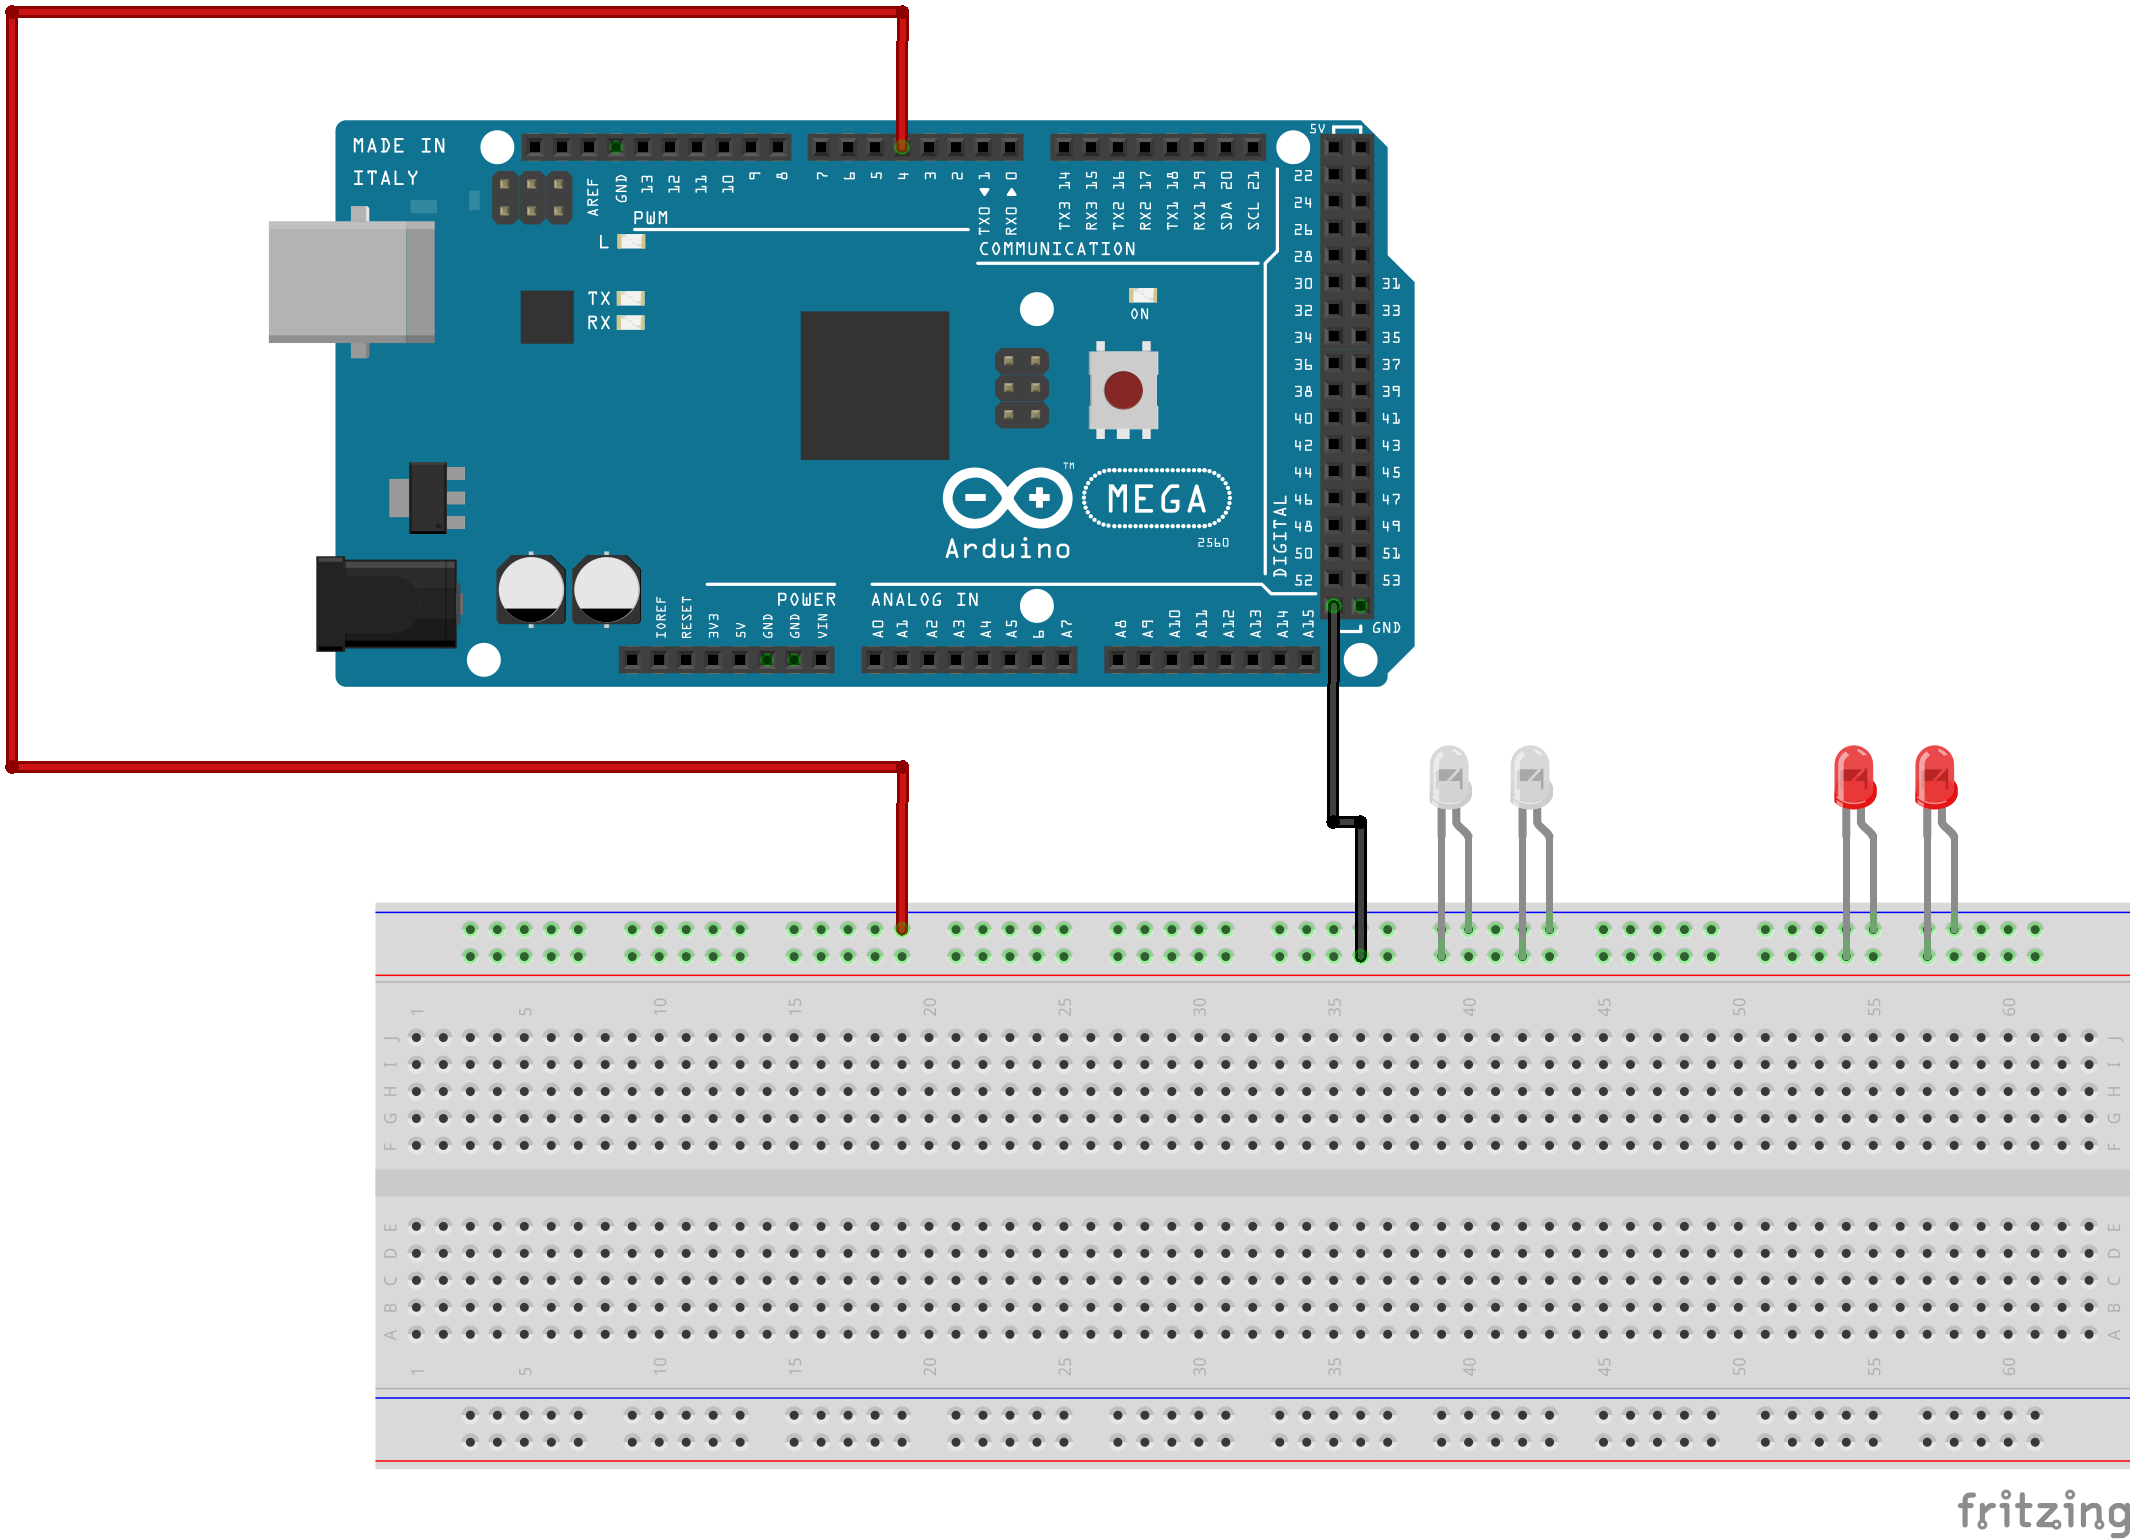
\includegraphics[scale=0.5]{imagenes/leds_conexion.png}
  \end{center}
  \caption{Conexionado de los leds de iluminación.}
  \label{img:leds_conexiones}
\end{figure}


\subsection{Puntero láser}

Junto con los leds de iluminación también se ha conectado un puntero láser accionable por el operador.


\subsubsection{Conexionado}

El conexionado del puntero láser se ha realizado del mismo modo que un para led convencional.\\

\begin{figure}[H]
  \begin{center}
   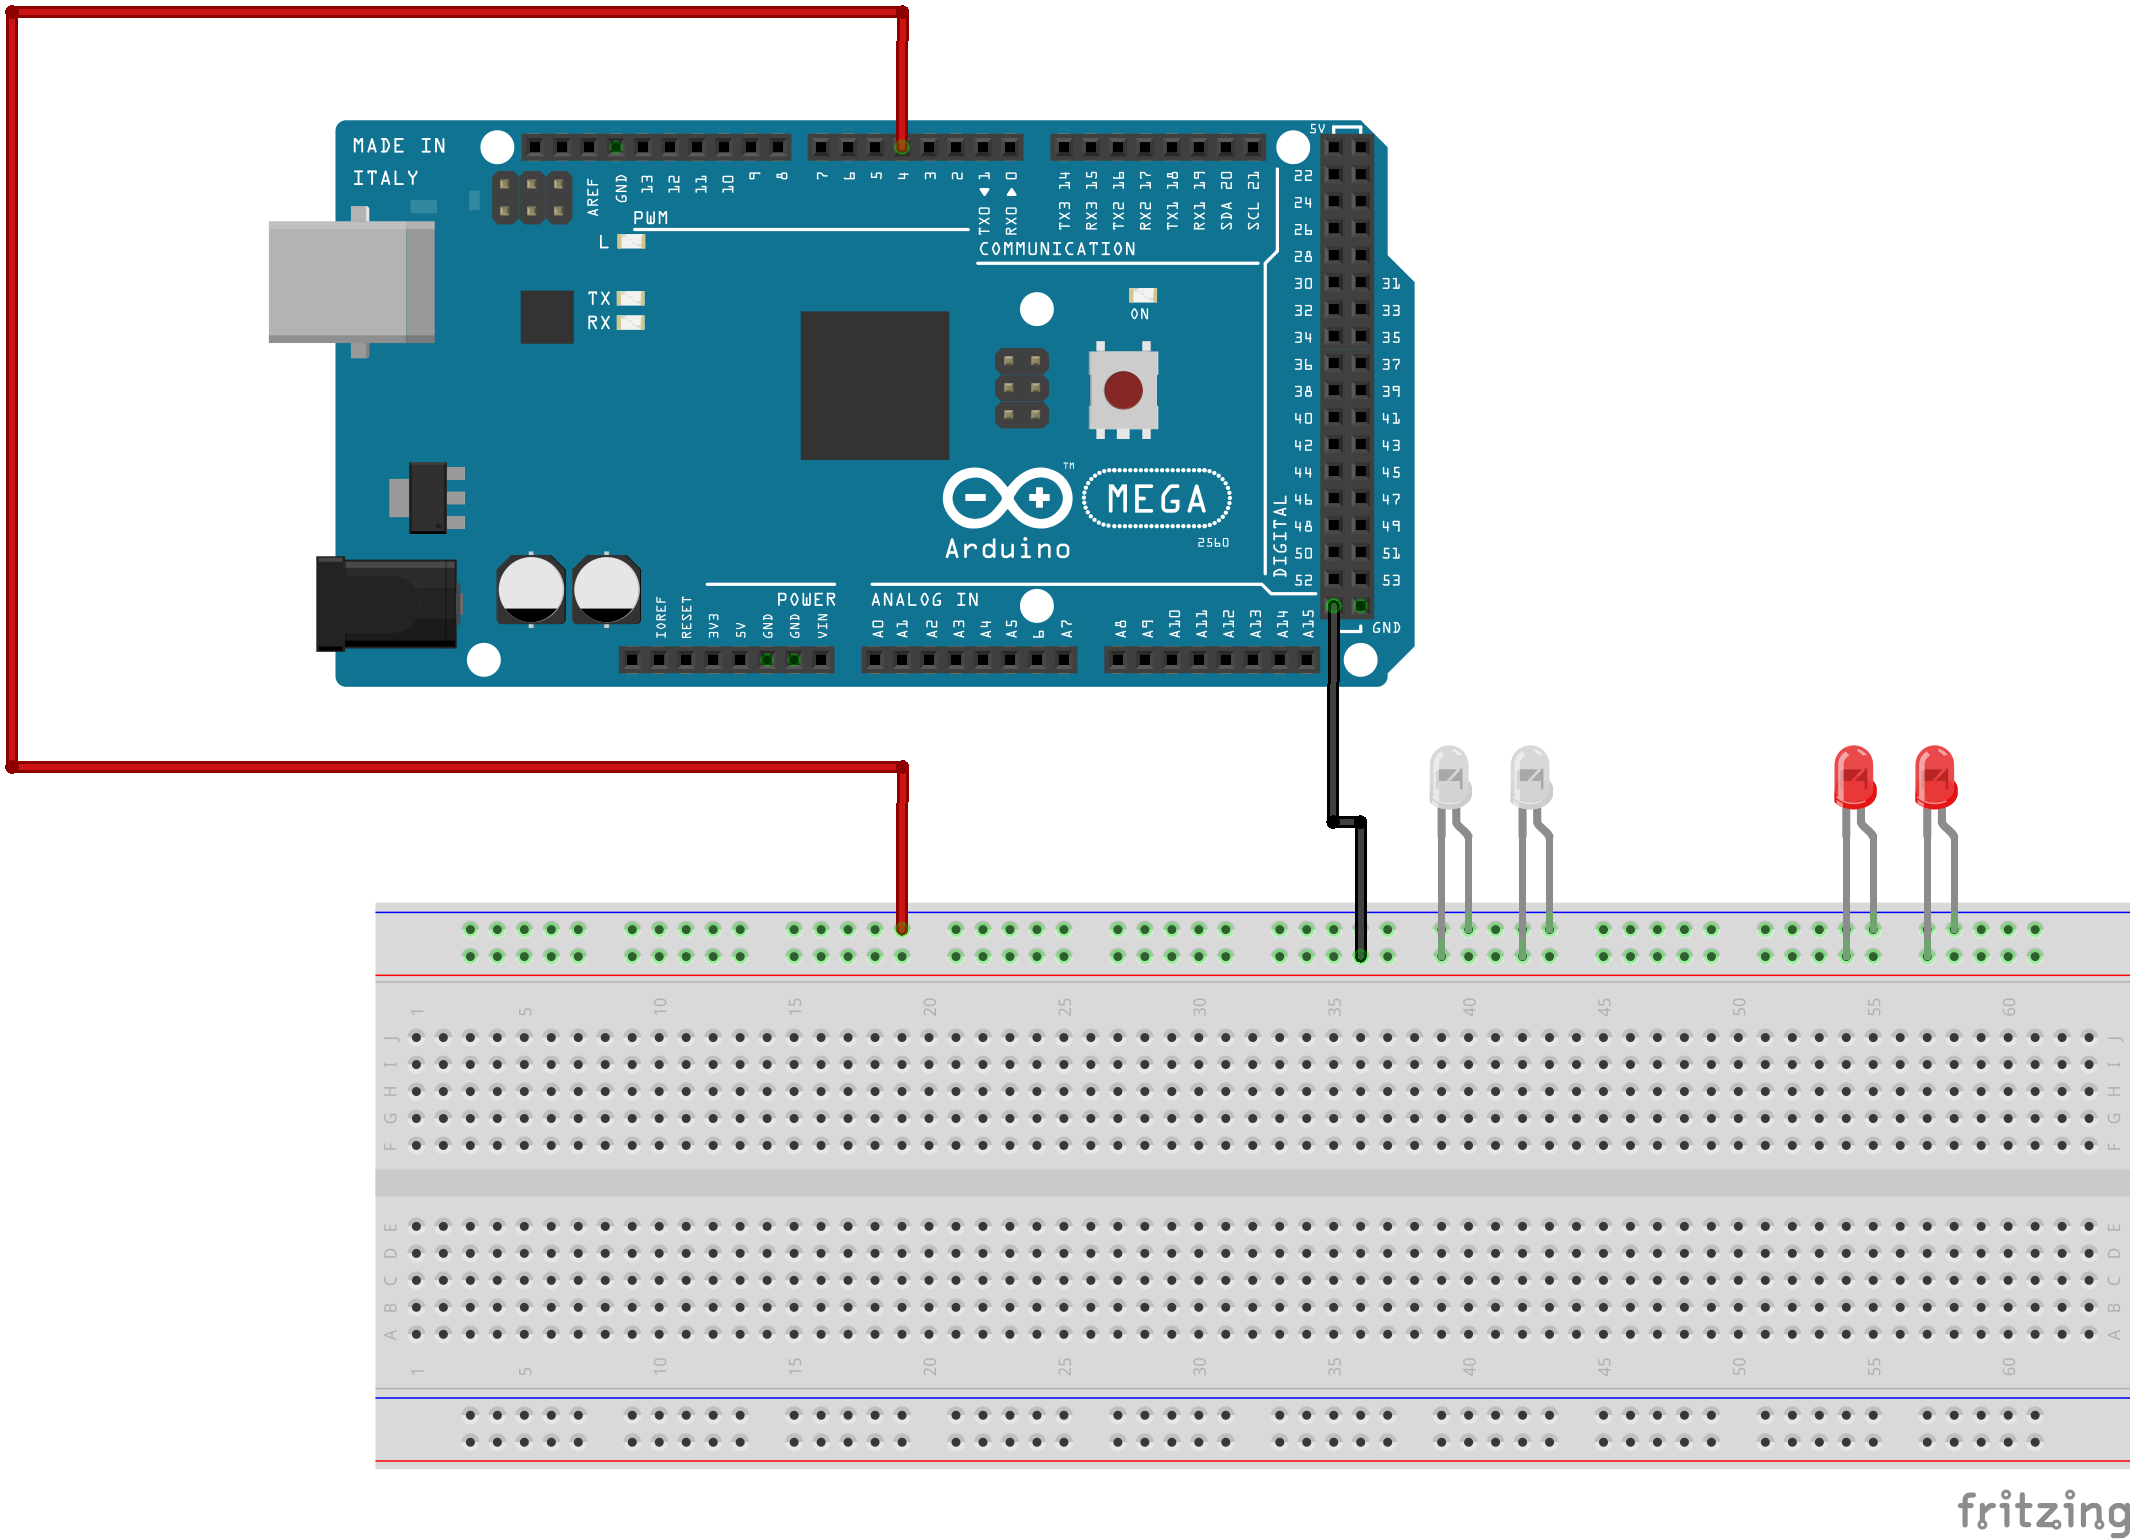
\includegraphics[scale=0.5]{imagenes/leds_conexion.png}
  \end{center}
  \caption{Conexionado de los leds de iluminación.}
  \label{img:leds_conexiones}
\end{figure}


\begin{figure}[H]
  \begin{center}
   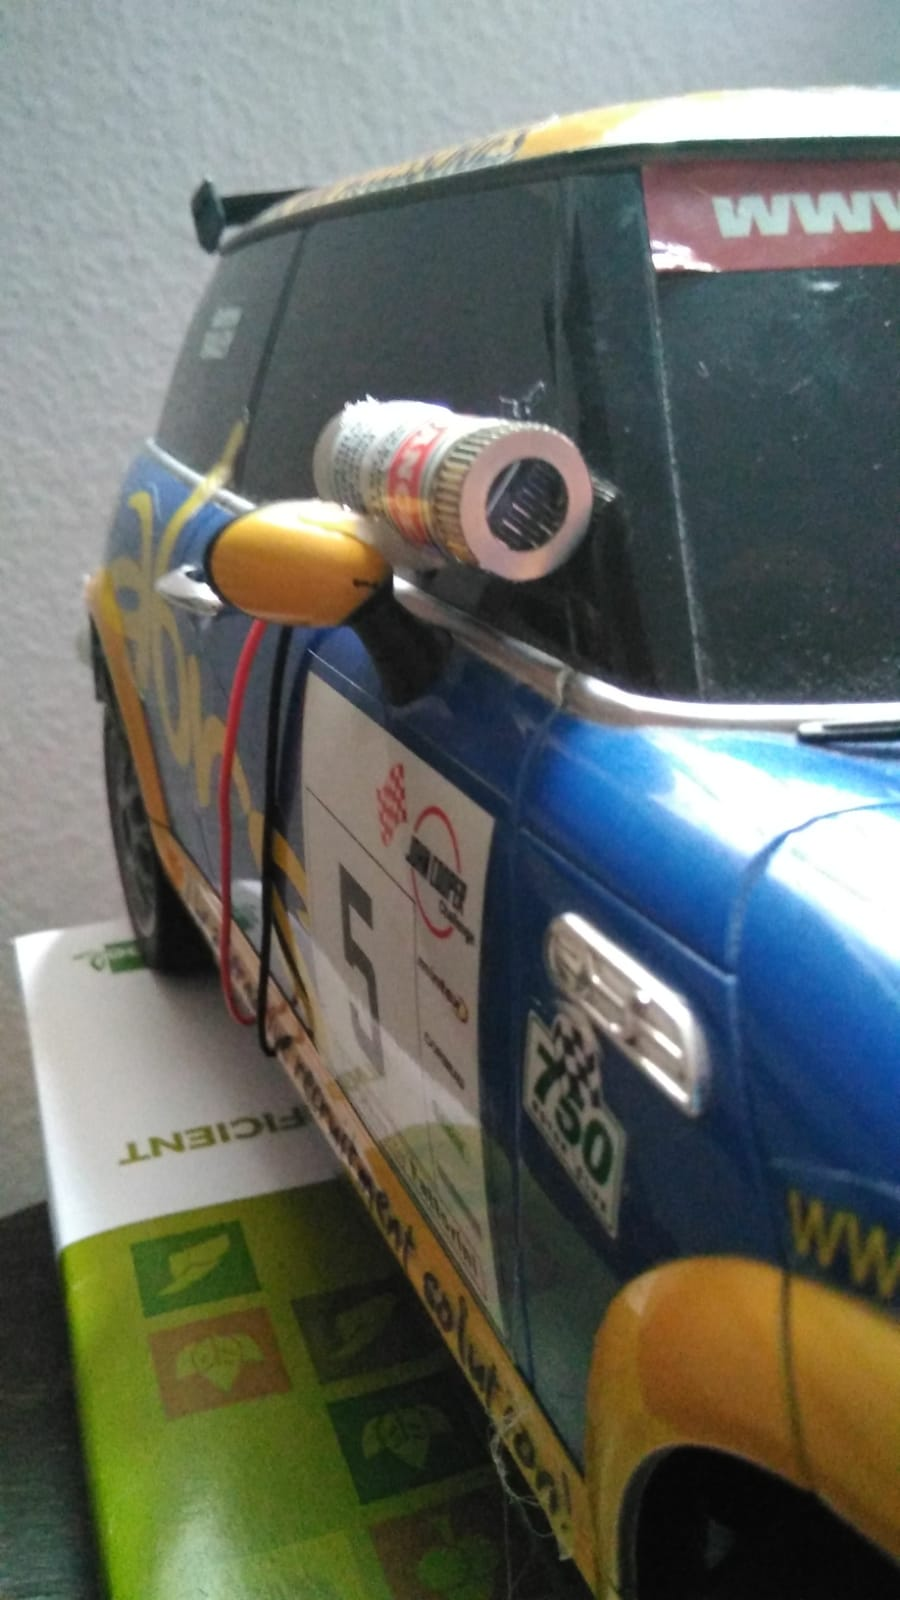
\includegraphics[scale=0.2]{imagenes/robot/puntero_laser.jpeg}
  \end{center}
  \caption{Vehículo SensorRS con el puntero láser situado en un lateral.}
  \label{vista-conexiones}
\end{figure}


\section{Sensores}

En la presente sección recogemos una descripción del funcionamiento y conexionado de los sensores más característicos utilizados en el proyecto.\\

\subsection{Sensores ultrasonidos}
\label{sec:ultrasonido}

Durante el movimiento del robot, es necesario la utilización de sensores de proximidad para
evitar la colisión con objetos. En este proyecto, los sensores empleados son dos sensores
ultrasonidos del modelo HC-SR04.\\

\begin{figure}[H]
  \begin{center}
    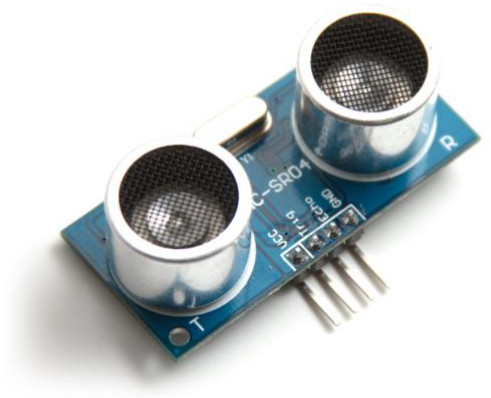
\includegraphics[scale=0.4]{imagenes/ultrasonido.jpg}
  \end{center}
  \caption{Sensores ultrasonidos empleados en el proyecto.}
  \label{figura:rpi-modulo-bateria}
\end{figure}

Los sensores irán dispuestos en la trasera del robot teniendo especial cuidado con las posibles interferencias entre dichos sensores, muy frecuentes debido a los rebotes. Es por ello
que se han situado en ambos laterales orientados hacia el exterior.\\

Para el correcto funcionamiento de estos sensores, se da un pulso de nivel alto de un mínimo de
10 μs en el pin al que se conecta el trig del sensor y a continuación se vuelve a poner a cero, tal y
como se especifica en el datasheet. Como consecuencia de este pulso, se generará otro pulso en
el pin de entrada donde se conecta la señal echo. El ancho del pulso recibido determina la
distancia a la que se encuentra el objeto, cuanto mayor es la duración del pulso más lejos se
encuentra el objeto. Utilizando una interrupción que se produzca por cada flanco de subida y
bajada, se puede obtener el ancho de dicho pulso y mediante el uso de un timer se puede medir el
tiempo transcurrido entre dichos flancos.\\

\begin{figure}[H]
  \begin{center}
    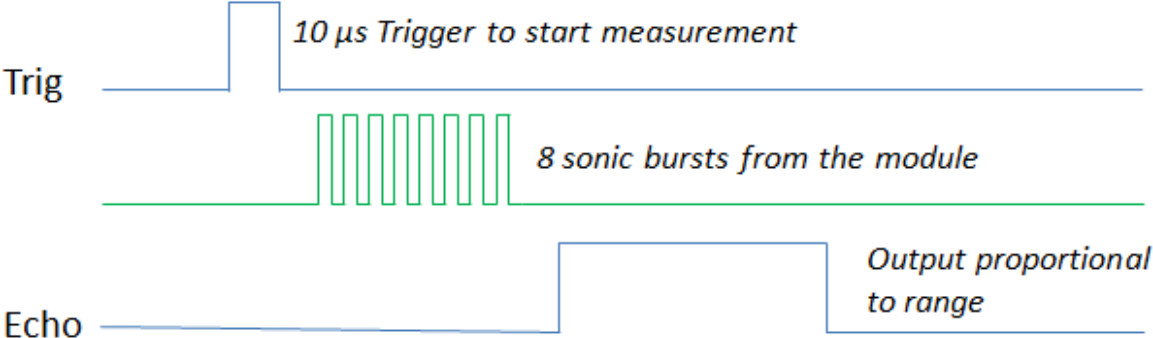
\includegraphics[scale=0.3]{imagenes/grafica_ultrasonido.jpg}
  \end{center}
  \caption{Pulsos para la correcta lectura del sensor ultrasonidos.}
  \label{figura:rpi-modulo-bateria}
\end{figure}

Para calcular la distancia a la que se encuentran los objetos situados frente al sensor, se emplea la
fórmula:\\

\begin{equation}
Distancia (cm) = \dfrac{tiempo (\mu s)}{58}
\end{equation}

En dicha fórmula, el tiempo se encuentra en microsegundos y la distancia a la que se encuentra
el objeto se obtiene en centímetros.\\

Otra forma de calcular la distancia sería utilizando la velocidad del sonido (340 m/s) y sabiendo
que la distancia que recorre es en sentido de ida y de vuelta, por tanto habría que dividir la
distancia calculada entre dos.\\

El comportamiento de la función encargada de medir la distancia de los sensores ultrasonidos se
puede descomponer en dos diagramas de flujo, uno encargado de dar los pulsos para iniciar la
lectura y otro que se encarga de medir la distancia.\\

Indicar que la distancia que se puede medir utilizando este sensor de proximidad
abarca el rango 2 cm – 400cm, tal y como se especifica en las características técnicas del mismo.\\

Por otra parte, es posible que objetos de pequeña dimensión o bien de superficie rugosa den problemas
a la hora de medir las distancias, debido a que no se refleja la señal o bien porque se producen
reflexiones.\\


\begin{figure}[H]
  \begin{center}
    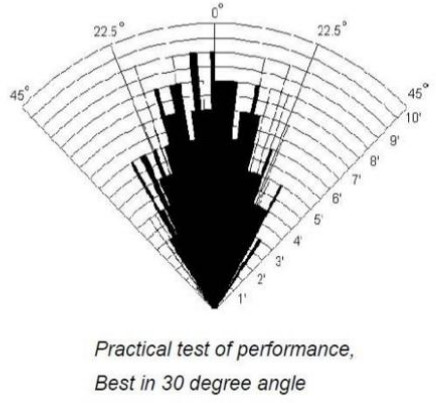
\includegraphics[scale=0.3]{imagenes/ultrasonido_directividad.jpg}
  \end{center}
  \caption{Directividad del sensor HCSR-04.}
  \label{figura:rpi-modulo-bateria}
\end{figure}

Los sensores ultrasonidos se emplearán tanto para medir distancias con los objetos próximos
como para detener el vehículo, si es necesario, cuando hay riesgo de colisión.\\

\subsubsection{Conexionado}

El sensor HC-SR04 dispone de 4 pines, la toma de tierra \textbf{GND}, pin de echo \texbf{ECHO}, trig \texbf{TRIG} y para la alimentación \textbf{VCC} 
(5V). En la siguiente imagen puedes ver el esquema de conexión con Arduino.

\begin{figure}[H]
  \begin{center}
    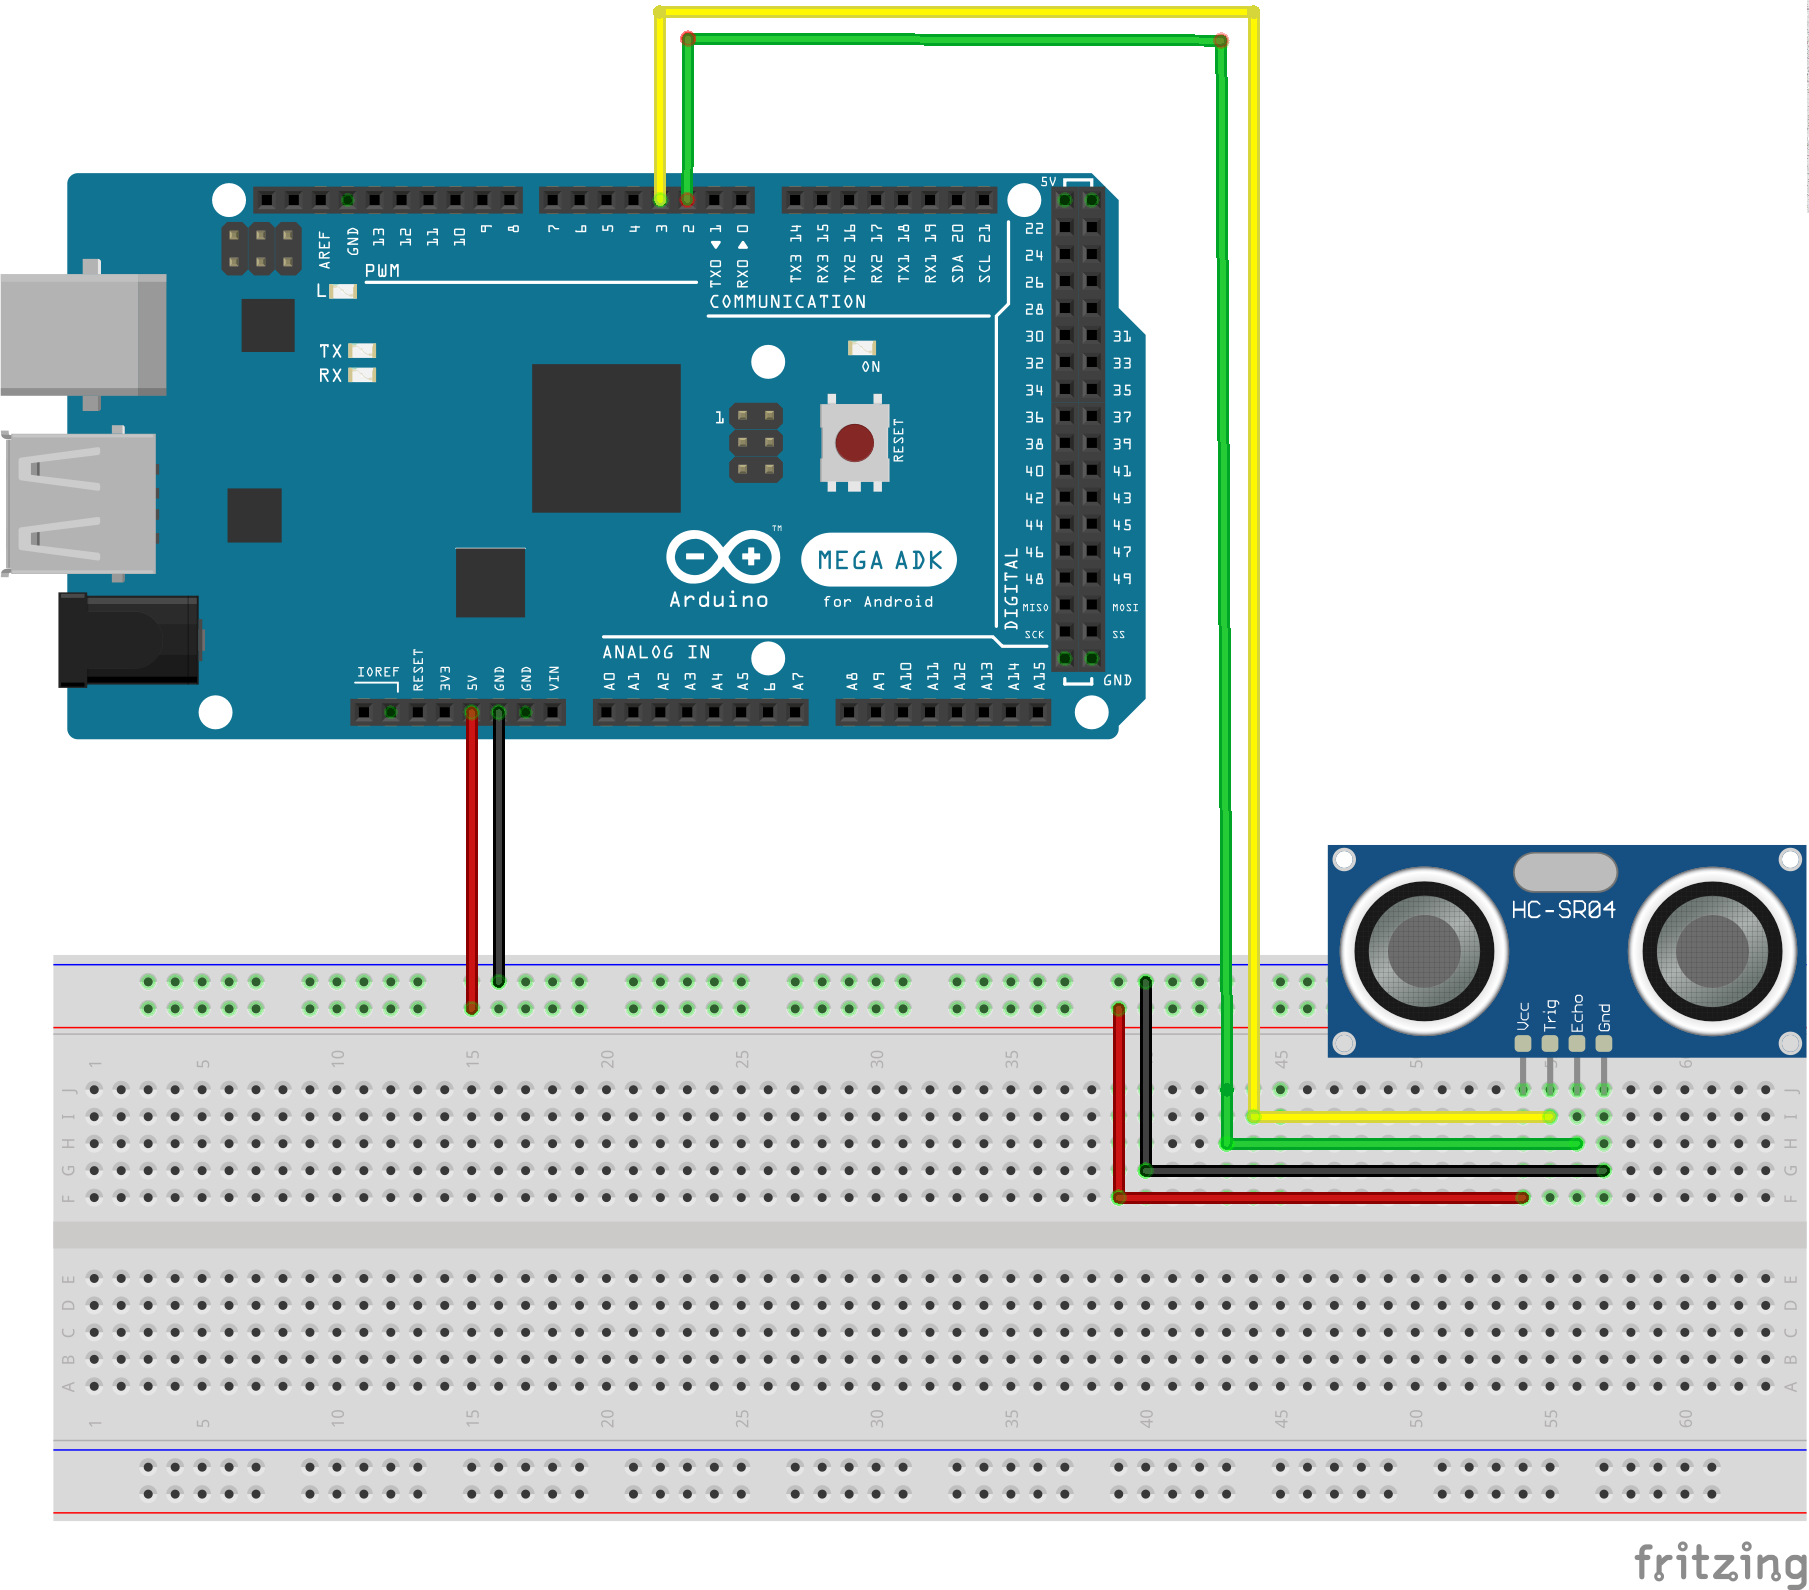
\includegraphics[scale=0.6]{imagenes/conexionado_ultrasonido.png}
  \end{center}
  \caption{Conexionado del sensor HC-SR04 con Arduino.}
  \label{figura:sensor_HC-SR04_conexionado}
\end{figure}


 \begin{figure}[H]
  \begin{center}
    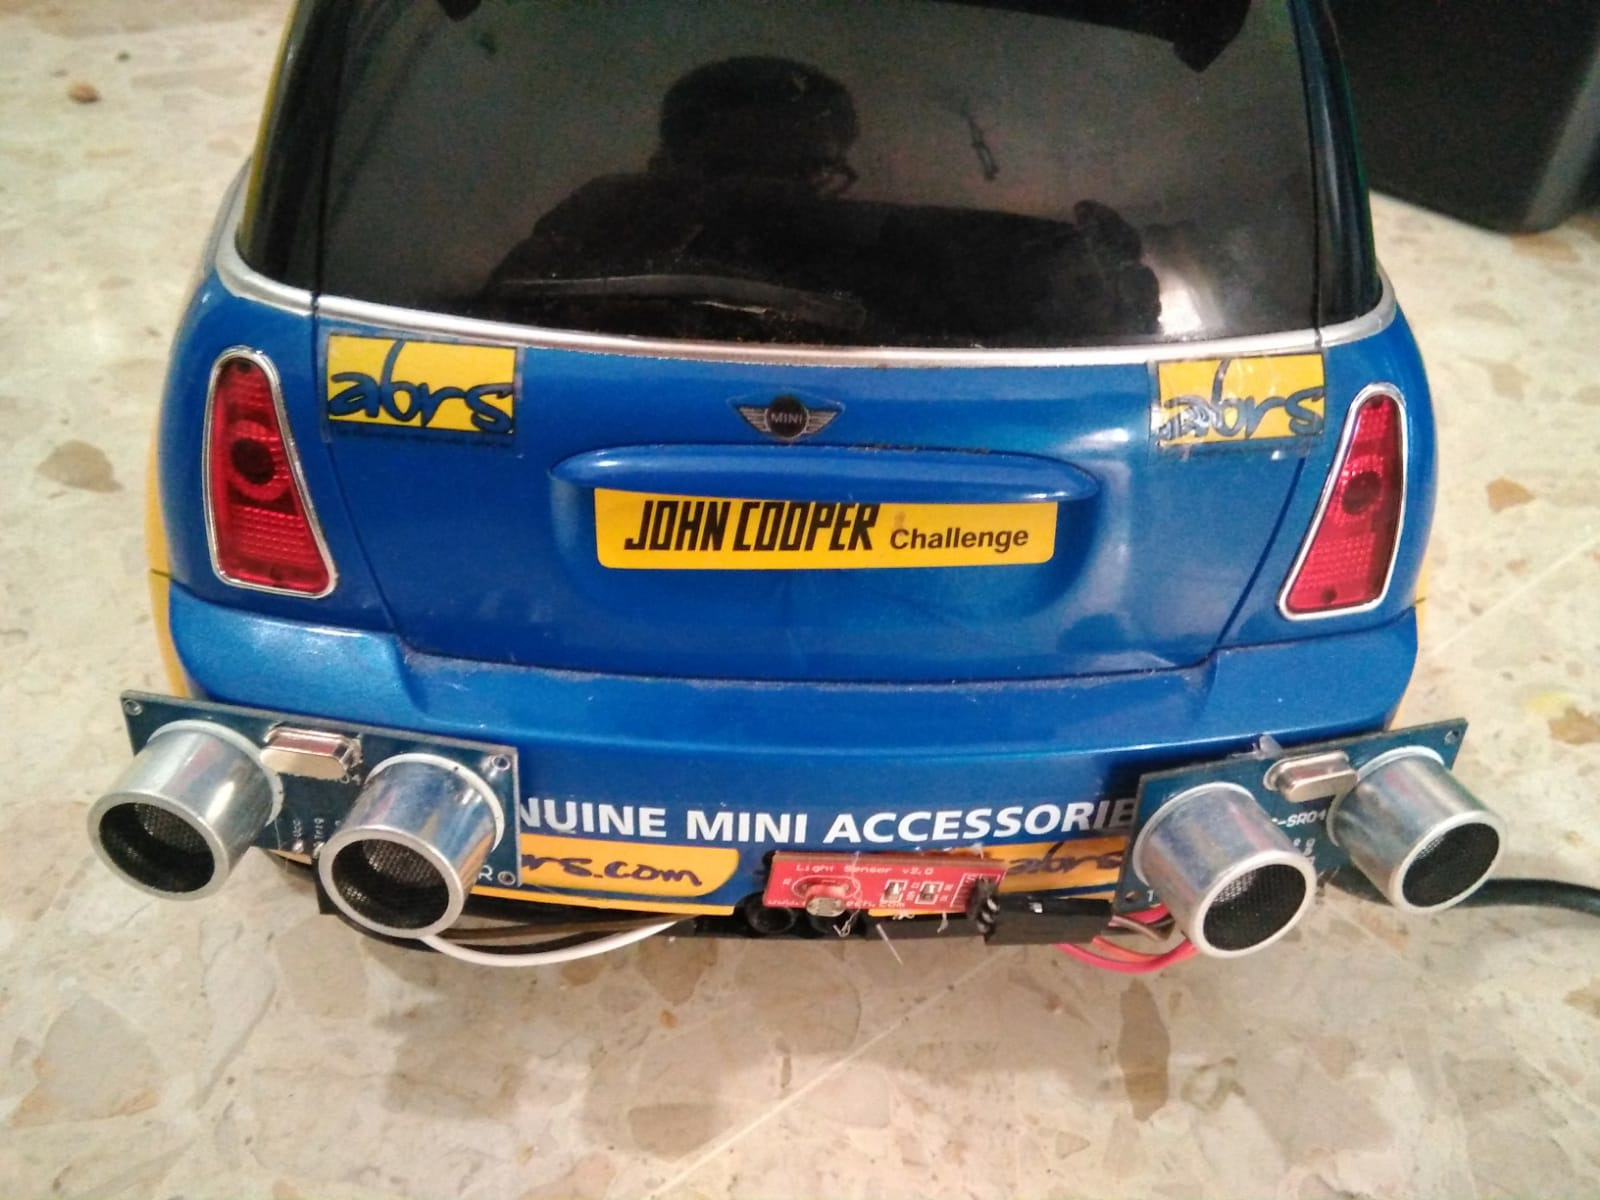
\includegraphics[scale=0.2]{imagenes/robot/ultrasonido_instalado.jpeg}
  \end{center}
  \caption{Sensores ultrasónicos situados en la parte trasera del vehículo.}
  \label{figura:sensor_mq_2_potenciometro}
\end{figure}

\subsection{Sensor de temperatura y humedad DHT11}
\label{sec:dth11}

% https://programarfacil.com/blog/arduino-blog/sensor-dht11-temperatura-humedad-arduino/

Para poder controlar la temperatura y la humedad relativa de la zona por la que se mueve el
robot, se ha decidido añadir un sensor de temperatura. En concreto se trata del sensor DHT11, que
se controla por un pin de propósito general y cuyas características se adjuntan en la referencia \ref{}.

\begin{figure}[H]
  \begin{center}
    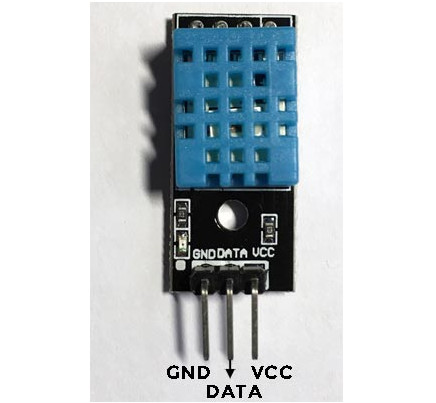
\includegraphics[scale=0.3]{imagenes/dth11.jpg}
  \end{center}
  \caption{Sensor de temperatura DHT11.}
  \label{figura:sensor_dth11}
\end{figure}

El sensor DHT11 en su versión PCB consta de tres pines. Un pin \textbf{VCC} de alimentación, uno \textbf{DATA} para la transferencia de
datos que se conecta al microcontrolador y un pin que conectado a tierra \textbf{GND}.\\

\subsubsection{transmisión de datos}

A pesar de que conectemos el pin de datos a un pin digital de nuestro microcontrolador, se trata de un dispositivo analógico. Dentro del propio dispositivo se hace la
conversión entre analógico y digital.\\

Por lo tanto, partimos de una señal analógica que luego es convertida en formato digital y se enviará al microcontrolador. La trama de datos es de 40 bits correspondiente a la
información de humedad y temperatura del DHT11.\\

\begin{figure}[H]
  \begin{center}
    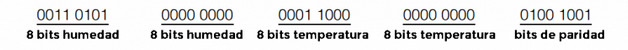
\includegraphics[scale=0.6]{imagenes/dth11_bits.jpg}
  \end{center}
  \caption{Disposición de los bits de datos del DHT11.}
  \label{figura:sensor_dth11_bits}
\end{figure}

El primer grupo de 8-bit es la parte entera de la humedad y el segundo grupo la parte decimal. Lo mismo ocurre con el tercer y cuarto grupo, la parte entera de la temperatura 
y la parte decimal. Por último los bits de paridad para confirmar que no hay datos corruptos.\\

Estos bits de paridad lo único que hacen es asegurarnos de que la información es correcta, sumando los 4 primero grupos de 8-bit. Esta suma debe ser igual a los bit de
paridad. Si nos centramos en la imagen anterior y sumamos los bits, comprobamos que todo está correcto.\\

\begin{equation}
0011 0101 + 0000 0000 + 0001 1000 + 0000 0000 = 0100 1101
\end{equation}

El sensor DHT11 tiene una resolución en el sensor de temperatura de un grado centígrado y en la
humedad relativa del 1 por ciento y se recomienda respetar un intervalo de al menos un segundo entre las
tomas de medidas para el correcto funcionamiento del dispositivo. Ante frecuencias de trabajo
mayores, se daña el dispositivo.\\

\subsubsection{Conexionado}

El sensor DHT11 integrado dentro de una PCB ya viene con la resistencia pull-up integrada. Esta resistencia puede resultar muy útil en ocasiones, pero si añadimos un cable
de más de 20 metros, deberemos tener en cuenta dicho factor.

Este modelo de DHT11, como comentamos anteriormente, dispone de 3 pines, la toma de tierra \textbf{GND}, para los datos \texbf{DATA} y para la alimentación \textbf{VCC} 
(de 3,5V a 5V). En la siguiente imagen puedes ver el esquema de conexión con Arduino.

\begin{figure}[H]
  \begin{center}
    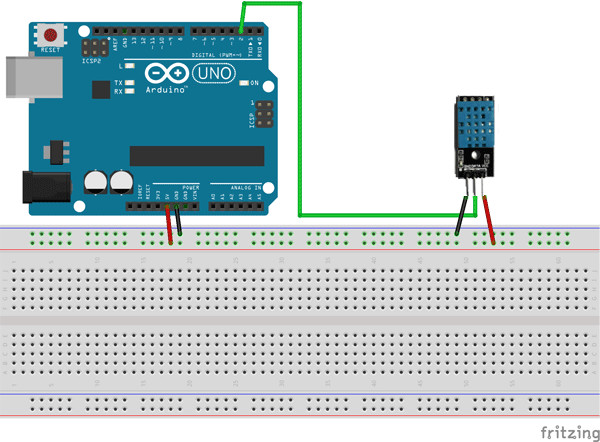
\includegraphics[scale=0.6]{imagenes/dth11_conexionado.jpg}
  \end{center}
  \caption{Conexionado de DHT11 con Arduino.}
  \label{figura:sensor_dth11_bits}
\end{figure}

\subsection{Sensor de gases}

% http://www.arduinohobby.com/deteccion-de-gas-con-arduino/

Para la detección de gas se ha empleado un sensor basado en la serie MQ ampliamente utilizados y bastante populares en muy diversas aplicaciones entre ellas incluida la robótica.
Existen una lista grande de sensores MQ donde cada uno fue diseñado para detectar un tipo de gas o sustancia especifica (o conjunto de ellas). El utilizado en el presente trabajo 
es un MQ-2 que detecta gases combustibles, incluyendo propano, butano, gas natural y humo. Para su activación y prueba basta con usar un encendedor para mostrar su operación. 
Otros modelos pueden detectar gases más raros como el hidrógeno o CO (monóxido de carbono), o incluso gases tóxicos como el amoníaco.\\

\begin{figure}[H]
  \begin{center}
    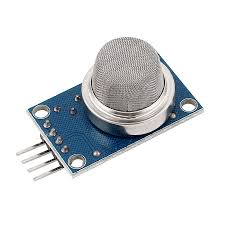
\includegraphics[scale=0.6]{imagenes/mq2_sensor.jpeg}
  \end{center}
  \caption{Sensor MQ-2.}
  \label{figura:sensor_mq_2}
\end{figure}

El sensor puede ser conectado de manera digital, analógica o mixta. Con la conexión digital podemos usarlo para detección de seguridad, con la analógica podemos medir la cantidad 
de gas en el aire en ppm (partes por millón), y si usamos ambos a la vez, podemos obtener una funcionalidad mixta.\\

Este tipo de sensores presentan la particularidad de que necesitan un tiempo de “calentamiento” antes de poder arrojar lecturas válidas. Es aconsejable un mínimo de 2 minutos
de calentamiento previo comenzando una vez alimentado el sensor. Trascurrido un par de minutos entonces se podrá realizar una medición efectiva.\\

En el presente proyecto nos hemos decantado por utilizar la detección de gas mediante el uso de su salida digital. Dicha salida digital, con nombre \textbf{D0}, tendrá un estado
0 o 1, representando 0 = 0v, y 1 = 5v aproximadamente, y que representan 0 = detección de gas, y 1 = sin detección de gas. 

\subsubsection{ Calibración del punto de detección de gas}

El sensor dispone de un potenciómetro (un componente que posee una ranura para su ajuste con un pequeño destornillador) que nos permite calibrar el umbral donde queremos que
notifique haber detectado gas. La calibración nos permite decidir el nivel de sensibilidad del módulo a la detección de gases.\\

La manera de calibrarlo es mientras está conectado, para ello simplemente giramos el potenciómetro hacia la izquierda hasta que un led se active, siendo
el testigo indicativo de detección de gas. El ajuste de la sensibilidad dependerá del resultado deseado, si se desea un mayor grado de sensibilidad, debemos girar hacia la derecha
hasta que se apague el led de testigo. Sin embargo si se quiere un mayor grado de tolerancia, se deberá girar hacia la derecha hasta el nivel deseado.\\

\begin{figure}[H]
  \begin{center}
    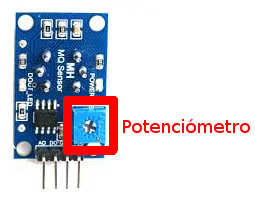
\includegraphics[scale=0.6]{imagenes/mq2_trasera.jpeg}
  \end{center}
  \caption{Vista del potenciómetro del sensor MQ-2.}
  \label{figura:sensor_mq_2_potenciometro}
\end{figure}

\subsubsection{Conexionado}

Conexionado del sensor MQ-2 en su modo digital. Siendo \textbf{D0} pin digital, \textbf{GND} a tierra y \txtbf{VCC} a alimentación 5V.\\

\begin{figure}[H]
  \begin{center}
    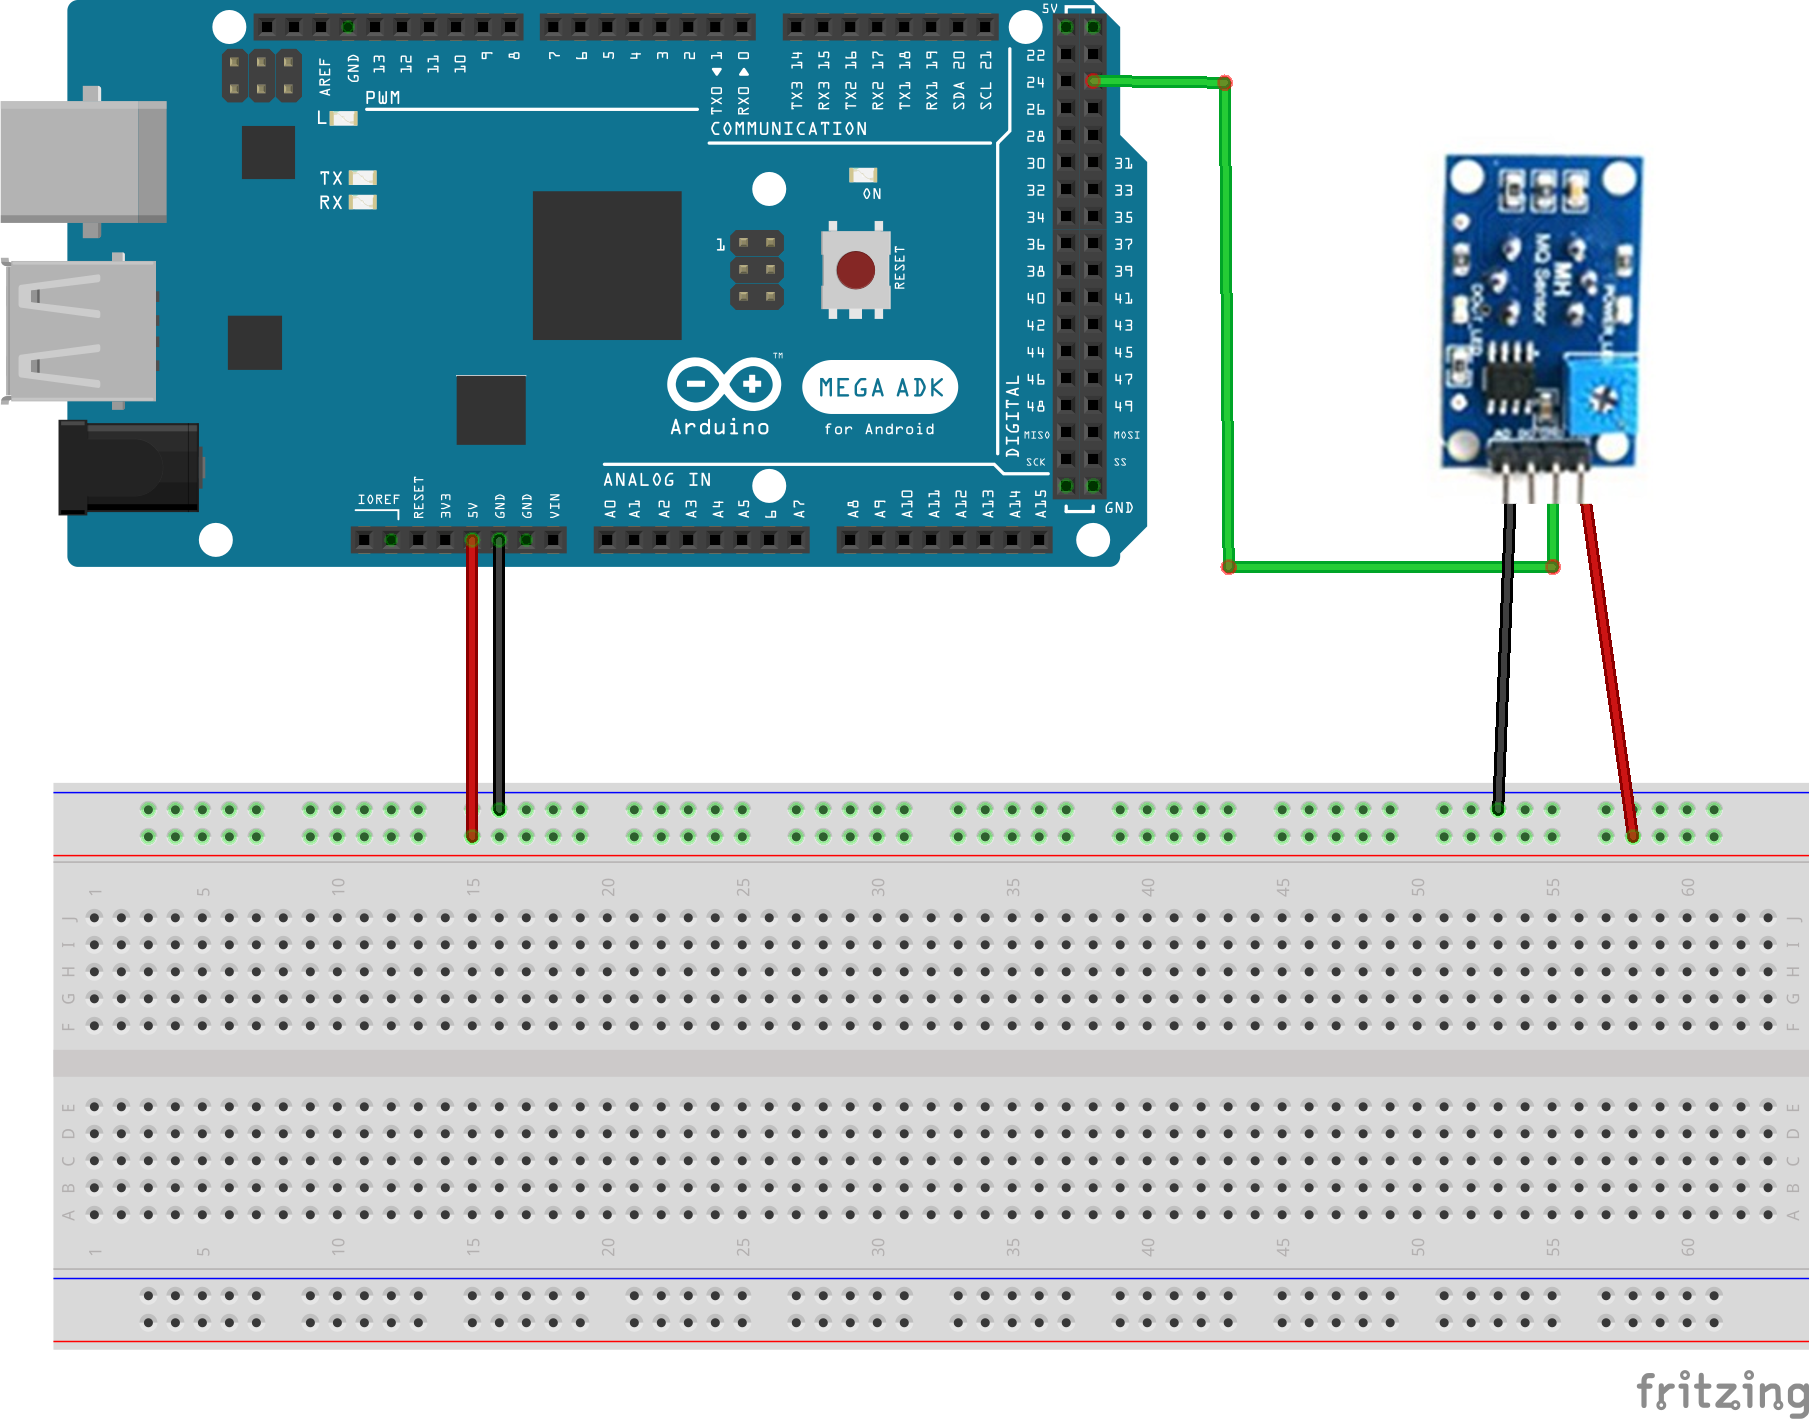
\includegraphics[scale=0.6]{imagenes/mq_2_conexionado.png}
  \end{center}
  \caption{Sensor MQ-2 utilizando el pin digital del microcontrolador.}
  \label{figura:mq_2_conexionado}
\end{figure}


\subsection{ Sensor de sonido }
%https://www.luisllamas.es/detectar-sonido-con-arduino-y-microfono-ky-038/

Para la detección de sonidos hemos empleado un micrófono el cual actúa como un transductor convirtiendo las ondas sonoras en señales eléctricas.\\

La salida producida por un micrófono es una señal eléctrica analógica que representa el sonido recibido. Sin embargo, esta señal suele ser demasiado baja para ser medida
siendo necesario amplificarla.\\

\begin{figure}[H]
  \begin{center}
    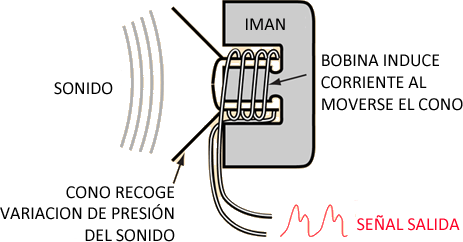
\includegraphics[scale=0.6]{imagenes/micro_amplificador.png}
  \end{center}
  \caption{Amplificación de la señal de audio recibida.}
  \label{figura:micro_amplificacion}
\end{figure}

La placa utilizada, KY-038 incorpora un micrófono junto con un comparador LM393, el cual permite obtener la lectura tanto analógica como digitalmente.\\

\begin{figure}[H]
  \begin{center}
    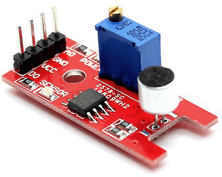
\includegraphics[scale=0.6]{imagenes/micro.png}
  \end{center}
  \caption{Vista del sensor de audio KY-038 utilizado.}
  \label{figura:micro_amplificacion}
\end{figure}

Los pines de los que dispone el sensor son: \textbf{AO}, Analog Output, \textbf{GND}, Ground, \textbf{VCC}, Alimentación de 3.3V a 12V y \textbf{DO}, Digital Output.\\

Lo más característico de este sensor es que la señal que nos entrega es digital y analógica, lo cual nos permite decidir cual utilizar según nuestras necesidades.
Si necesitamos saber el valor del sensor, podremos utilizar directamente la salida analógica para conseguir los datos crudos. Sino, podemos utilizar la salida digital, la cual
se activa o se desactiva según si el sensor llega a medir la intensidad del sonido que le configuremos, mediante la definición de la sensibilidad del sensor, de igual modo al sensor de detección de gases. \\

\subsubsection{Conexionado}

Conexionado del sensor KY-038 en su modo digital:

\begin{figure}[H]
  \begin{center}
    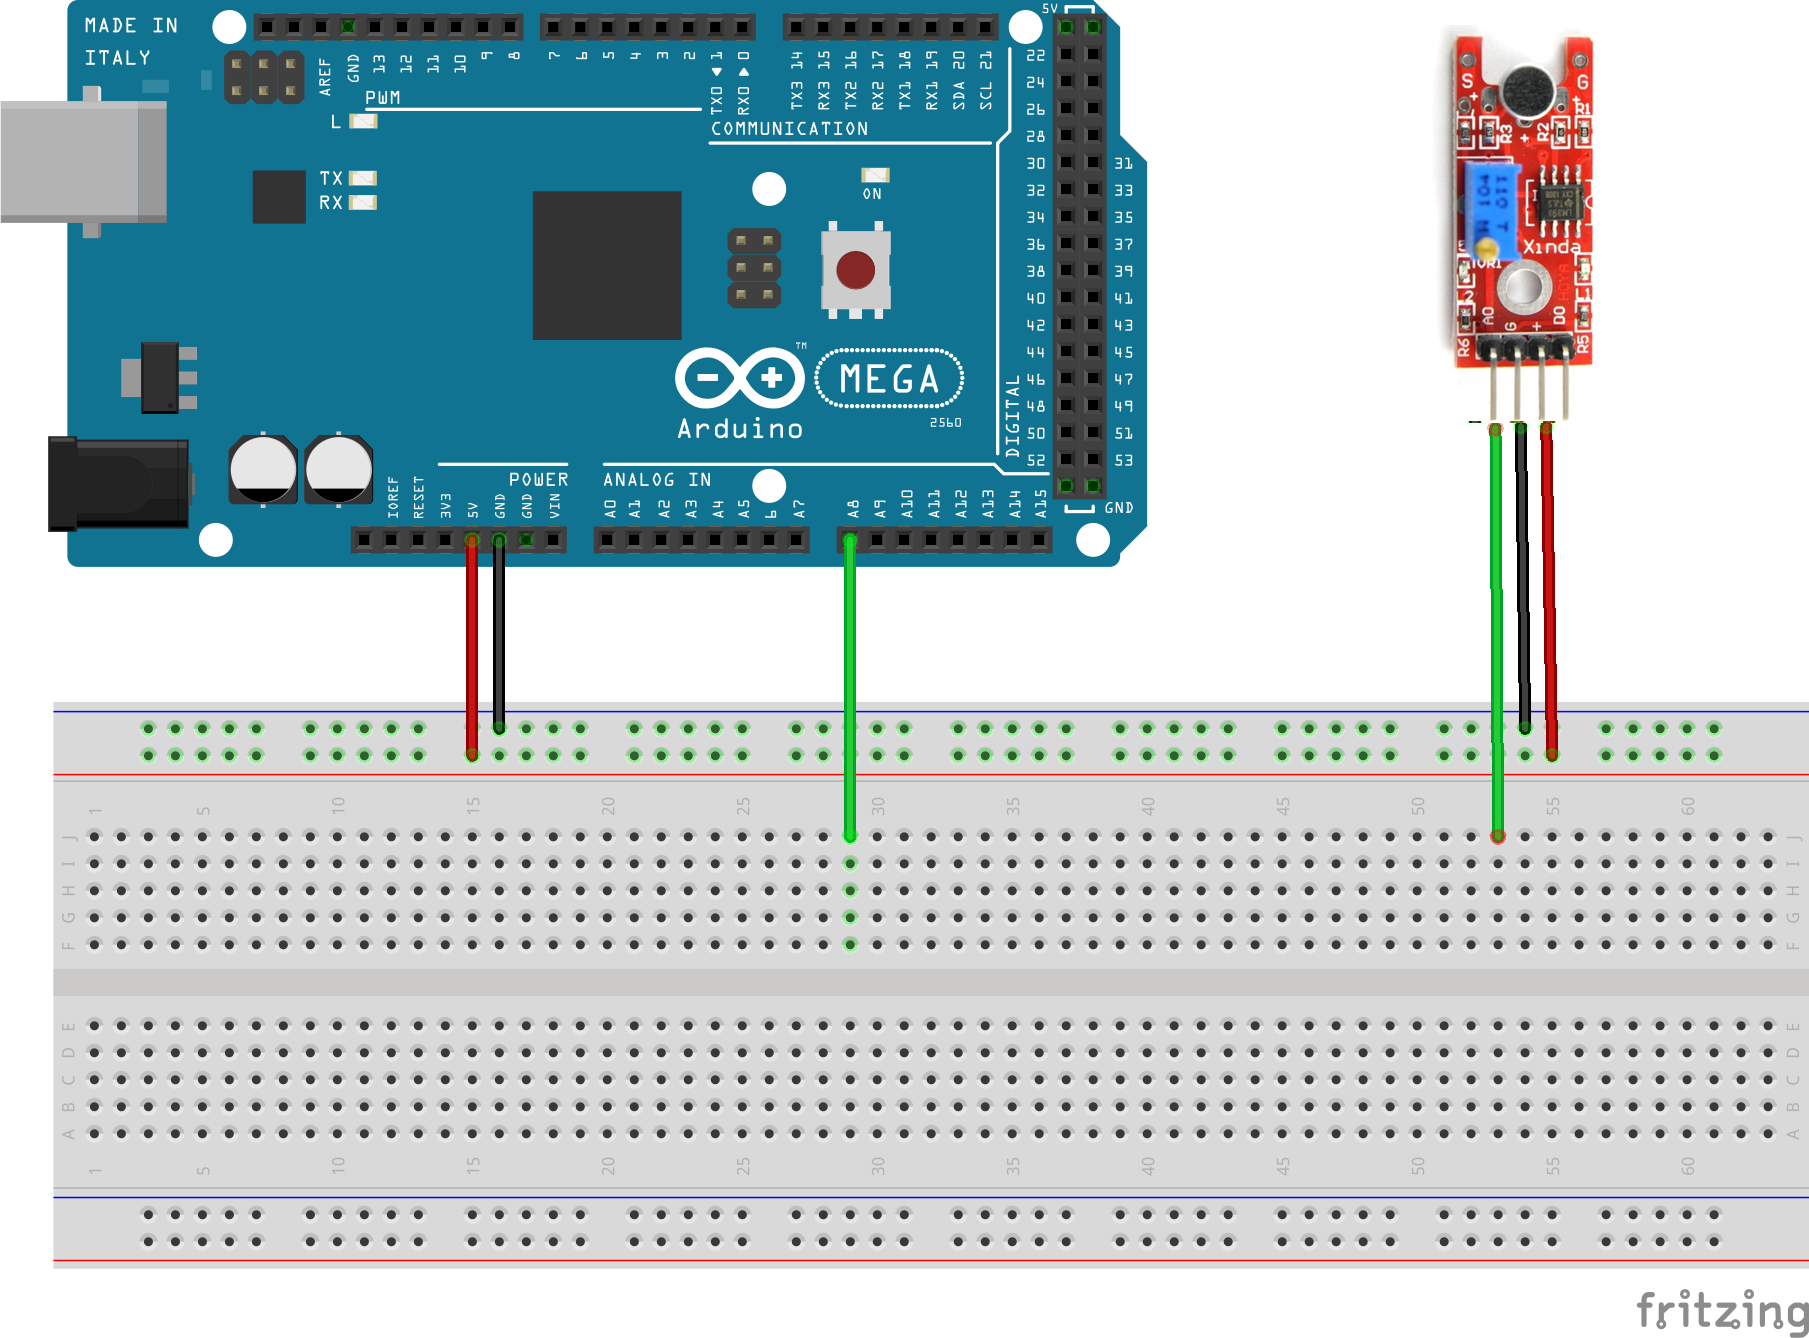
\includegraphics[scale=0.6]{imagenes/micro_conexionado.png}
  \end{center}
  \caption{Sensor KY-038 utilizando el pin digital del microcontrolador.}
  \label{figura:mq_2_conexionado}
\end{figure}


\subsection{Fotoresistor}

Un fotoresistor, o LDR (light-dependent resistor) es un dispositivo cuya resistencia varía en función de la luz recibida. Podemos usar esta variación para medir, a través de 
las entradas analógicas, una estimación del nivel del luz percibida en el entorno del vehículo siendo de utilidad para el encendido automático de la iluminación en aquellas situaciones 
donde resulte necesaria.\\

Un fotoresistor está formado por un semiconductor, típicamente sulfuro de cadmio CdS. Al incidir la luz sobre él algunos de los fotones son absorbidos, provocando que electrones pasen
a la banda de conducción y, por tanto, disminuyendo la resistencia del componente. Por tanto, un fotoresistor disminuye su resistencia a medida que aumenta la luz sobre él.
Los valores típicos son de 1 Mohm en total oscuridad, a 50-100 Ohm bajo luz brillante.\\


\begin{figure}[H]
  \begin{center}
    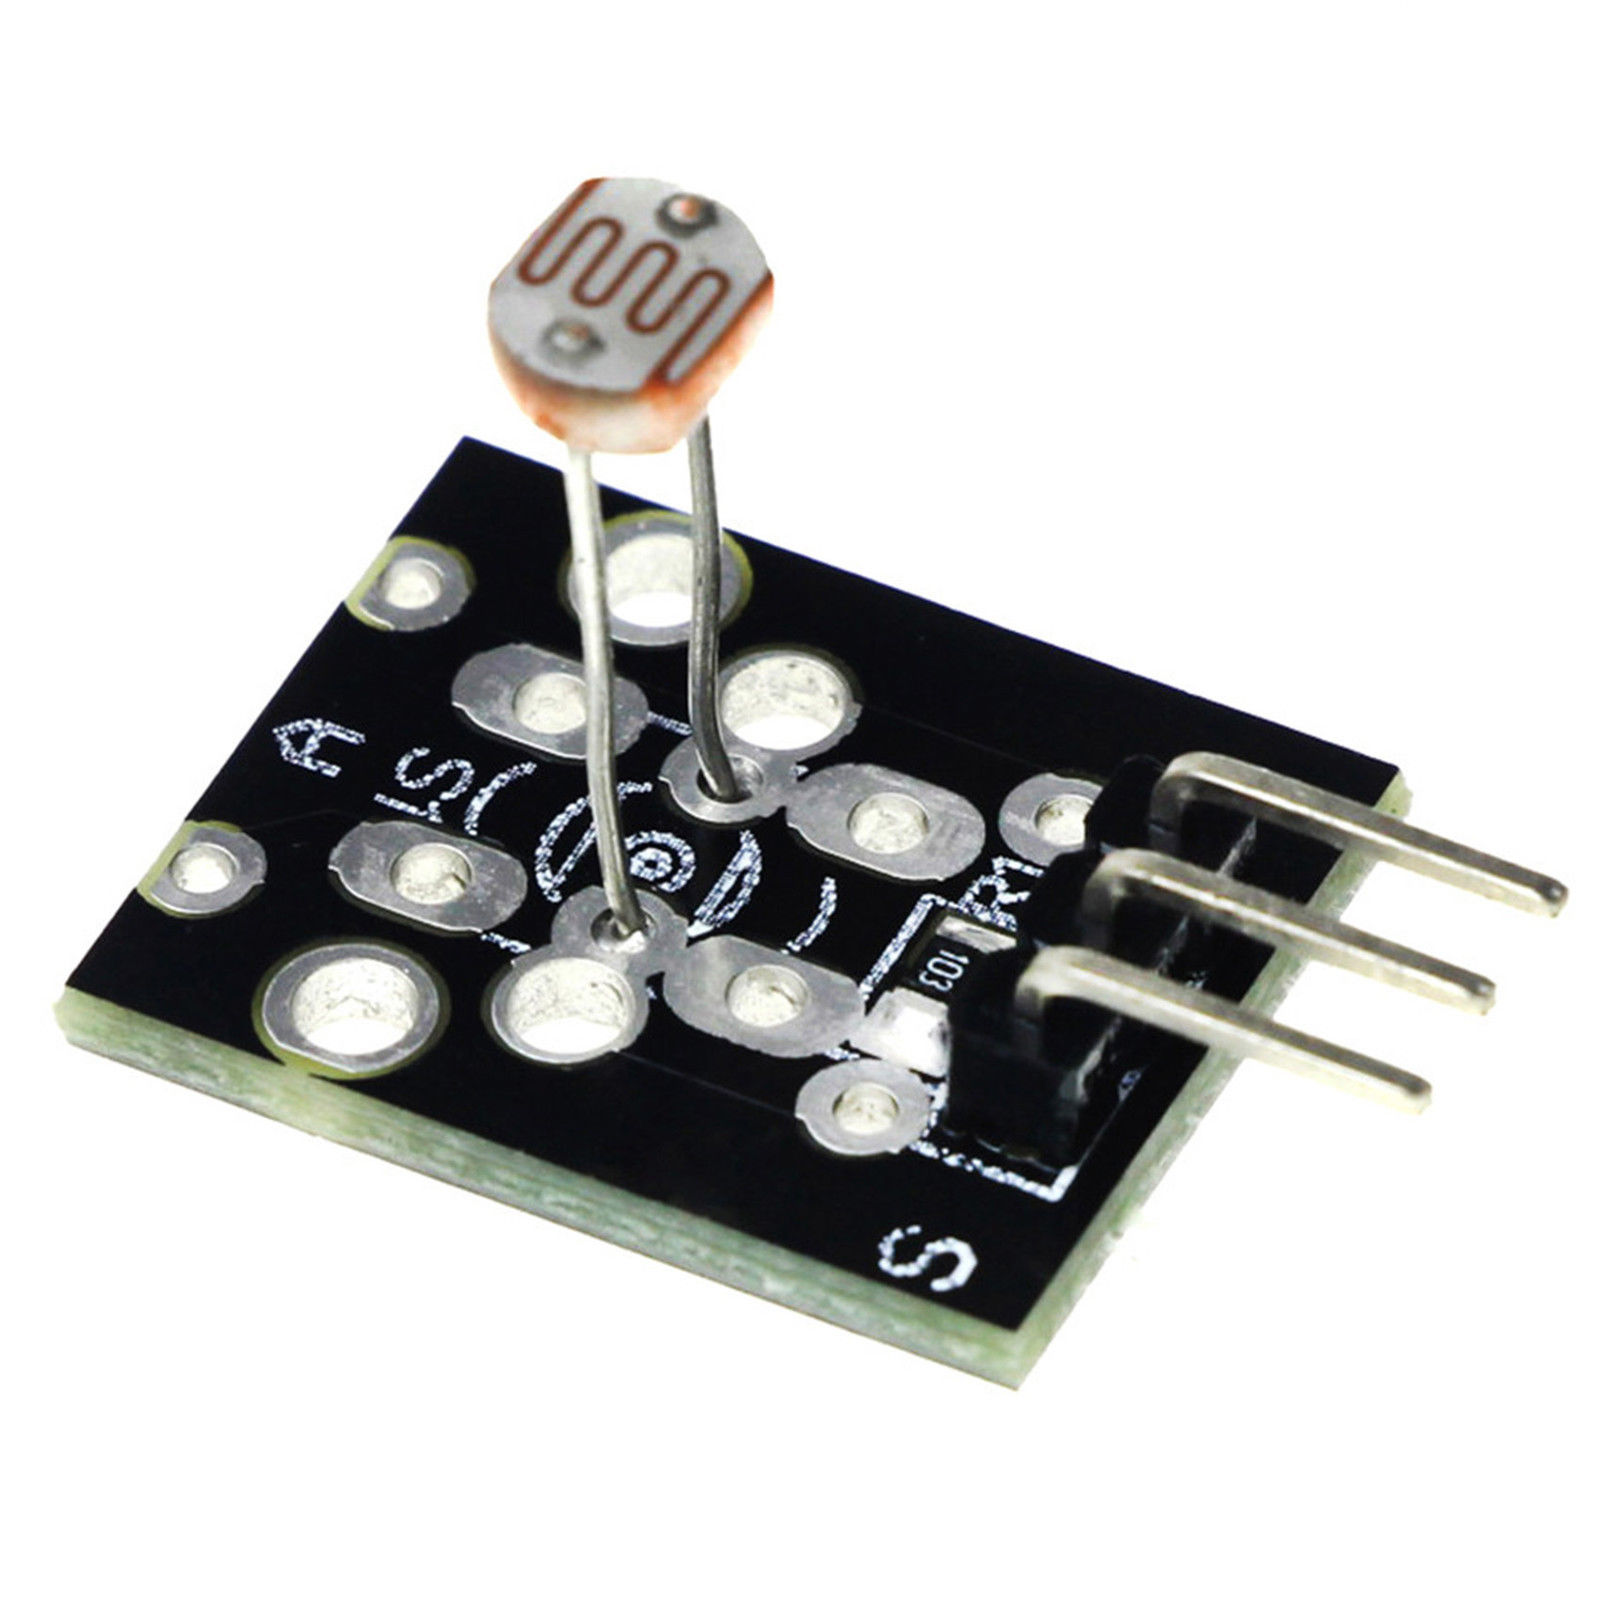
\includegraphics[scale=0.05]{imagenes/fotoresistor_utilizado.jpg}
  \end{center}
  \caption{Vista del fotoresistor utilizado.}
  \label{figura:micro_amplificacion}
\end{figure}


Por tanto, un fotoresistor disminuye su resistencia a medida que aumenta la luz sobre él. Los valores típicos son de 1 Mohm en total oscuridad, a 50-100 Ohm bajo condiciones de 
luz brillante.\\

\subsubsection{Conexionado}

Conexionado del fotoresistor a la placa Arduino:

\begin{figure}[H]
  \begin{center}
    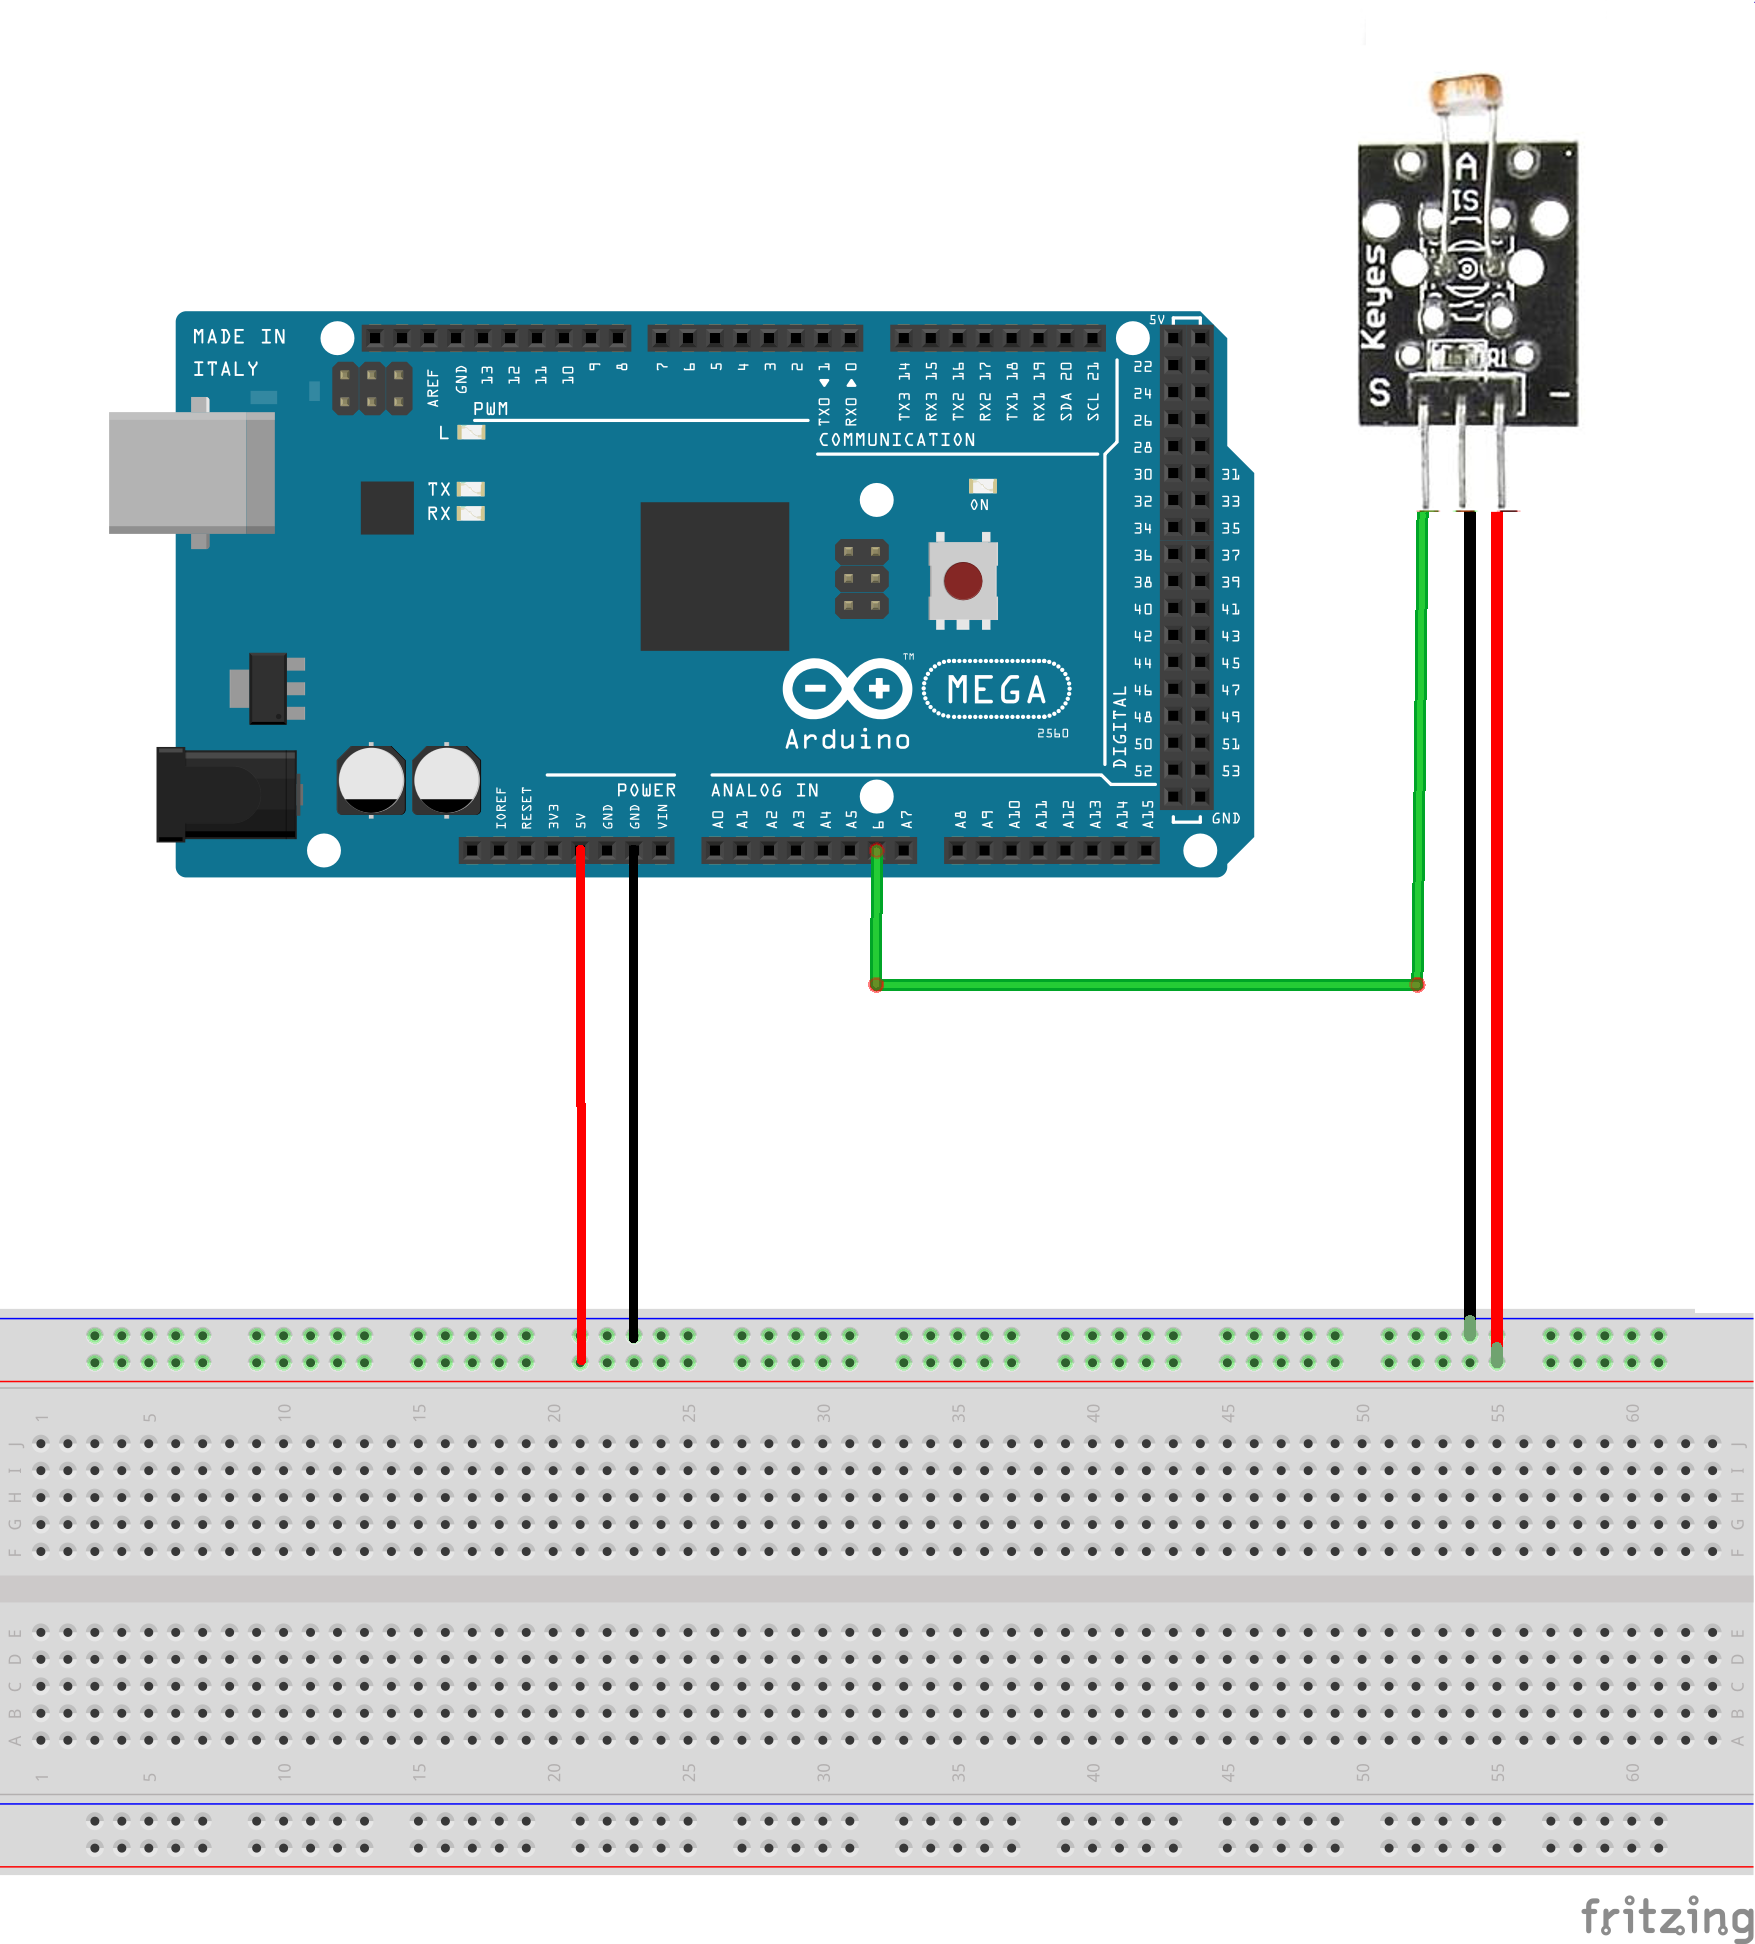
\includegraphics[scale=0.5]{imagenes/fotoresistor_conexionado.png}
  \end{center}
  \caption{Vista del fotoresistor utilizado.}
  \label{figura:micro_amplificacion}
\end{figure}


\subsection{Sensor de llama}

Un sensor de llama óptico es un dispositivo que permite detectar la existencia de combustión por la luz emitida por la misma. Esta luz puede ser detectada por un sensor óptico, 
y ser capturado por las entradas digitales y las entradas analógicas de Arduino.\\

La llama es un fenómeno de emisión de luz asociado a los procesos de combustión siendo ésta un proceso que desprende grandes cantidades de energía en forma de calor generándose
compuestos intermedios que liberan parte de su energía mediante la emisión de luz.\\

El espectro de emisión de la llama generada depende de los elementos que intervienen en la reacción. En el caso de combustión de productos con carbón en presencia del oxígeno 
tenemos dos picos característicos en ultravioleta en longitudes de onda de 185nm-260nm y en infrarrojo en longitudes de onda 4400-4600nm.\\

\begin{figure}[H]
  \begin{center}
    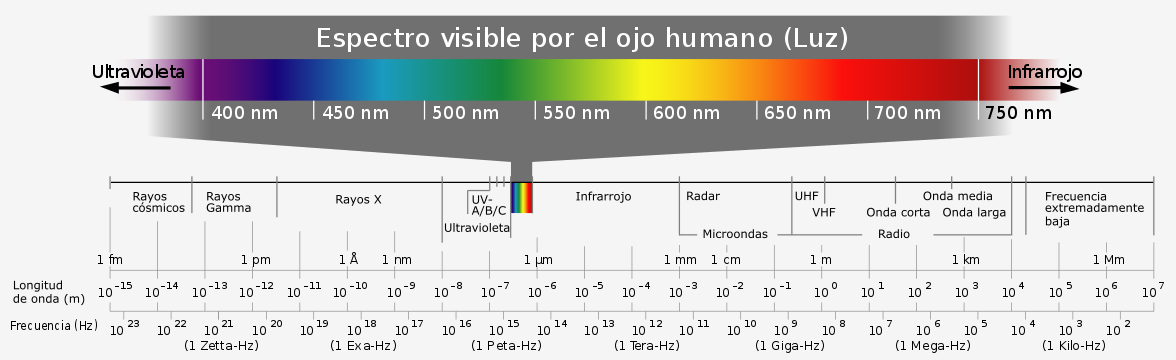
\includegraphics[scale=0.4]{imagenes/espectro.png}
  \end{center}
  \caption{Espectro visible por el ojo humano.}
  \label{fig:}
\end{figure}

Estos dispositivos se ajustan a las longitudes de onda características de la aparición de la llama y normalmente combinan las señales ultravioleta y de infrarrojo.\\
 
 \begin{figure}[H]
  \begin{center}
    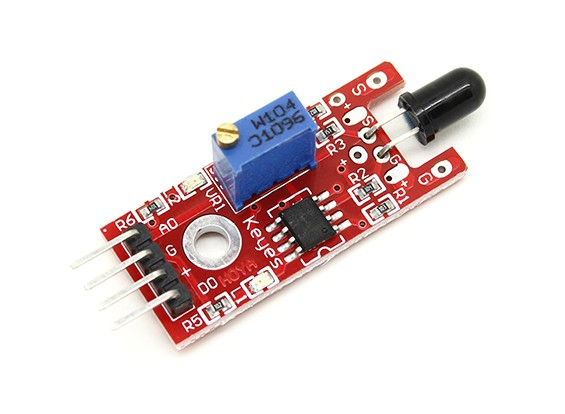
\includegraphics[scale=0.5]{imagenes/sensor_llama.jpg}
  \end{center}
  \caption{Vista del sensor de llama YG1006 utilizado.}
  \label{figura:sensor_mq_2_potenciometro}
\end{figure}

Estos sensores constan únicamente de un sensor infrarrojo ajustado al rango de los 760-1100 nm siendo su ángulo de detección de 60º, y la distancia de detección entre 0.40 m a 0.80.\\

Este tipo de sensores de llama infrarrojos suelen incorporar una placa de medición estándar con el comparador LM393, que permite obtener la lectura tanto como un valor analógico
como de forma digital cuando se supera un cierto umbral, que se regula a través de un potenciómetro ubicado en la placa.\\

 \begin{figure}[H]
  \begin{center}
    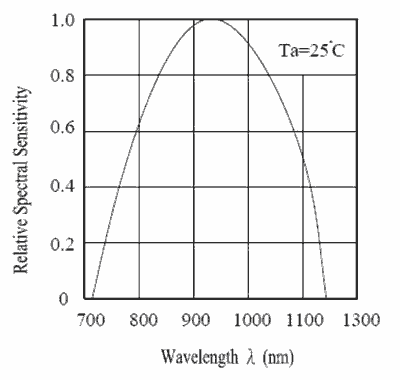
\includegraphics[scale=1.5]{imagenes/longitudes_onda.png}
  \end{center}
  \caption{Gráfico de sensibilidad espectral del sensor YG1006.}
  \label{figura:longitudes_onda}
\end{figure}

Como vemos en la figura \ref{figura:longitudes_onda}, las longitudes de onda de estos sensores poco tienen que ver con las emisiones características de las llamas, las cuales
pueden variar su espectro según múltiples factores siendo uno de ellos el material en combustión. Pudiéndose abarcar espectros desde tonos azulados de las llamas de gas a los
verdosos producidos por el sulfato de cobre. De hecho, estos sensores también son afectados incluso por la iluminación interior, dando lugar a numerosos falsos positivos.\\

Por tanto, la sensibilidad y fiabilidad de estos detectores de reducido coste no resultan suficientes para considerarlos un auténtico dispositivo de seguridad.\\
 
\subsubsection{Conexionado}

El esquema eléctrico es muy simple. Debemos alimentar el módulo conectando \textbf{GND} y \textbf{VCC} a los pines correspondientes de Arduino y salida \textbf{D0} a una de las 
entradas digitales de Arduino.\\

 \begin{figure}[H]
  \begin{center}
    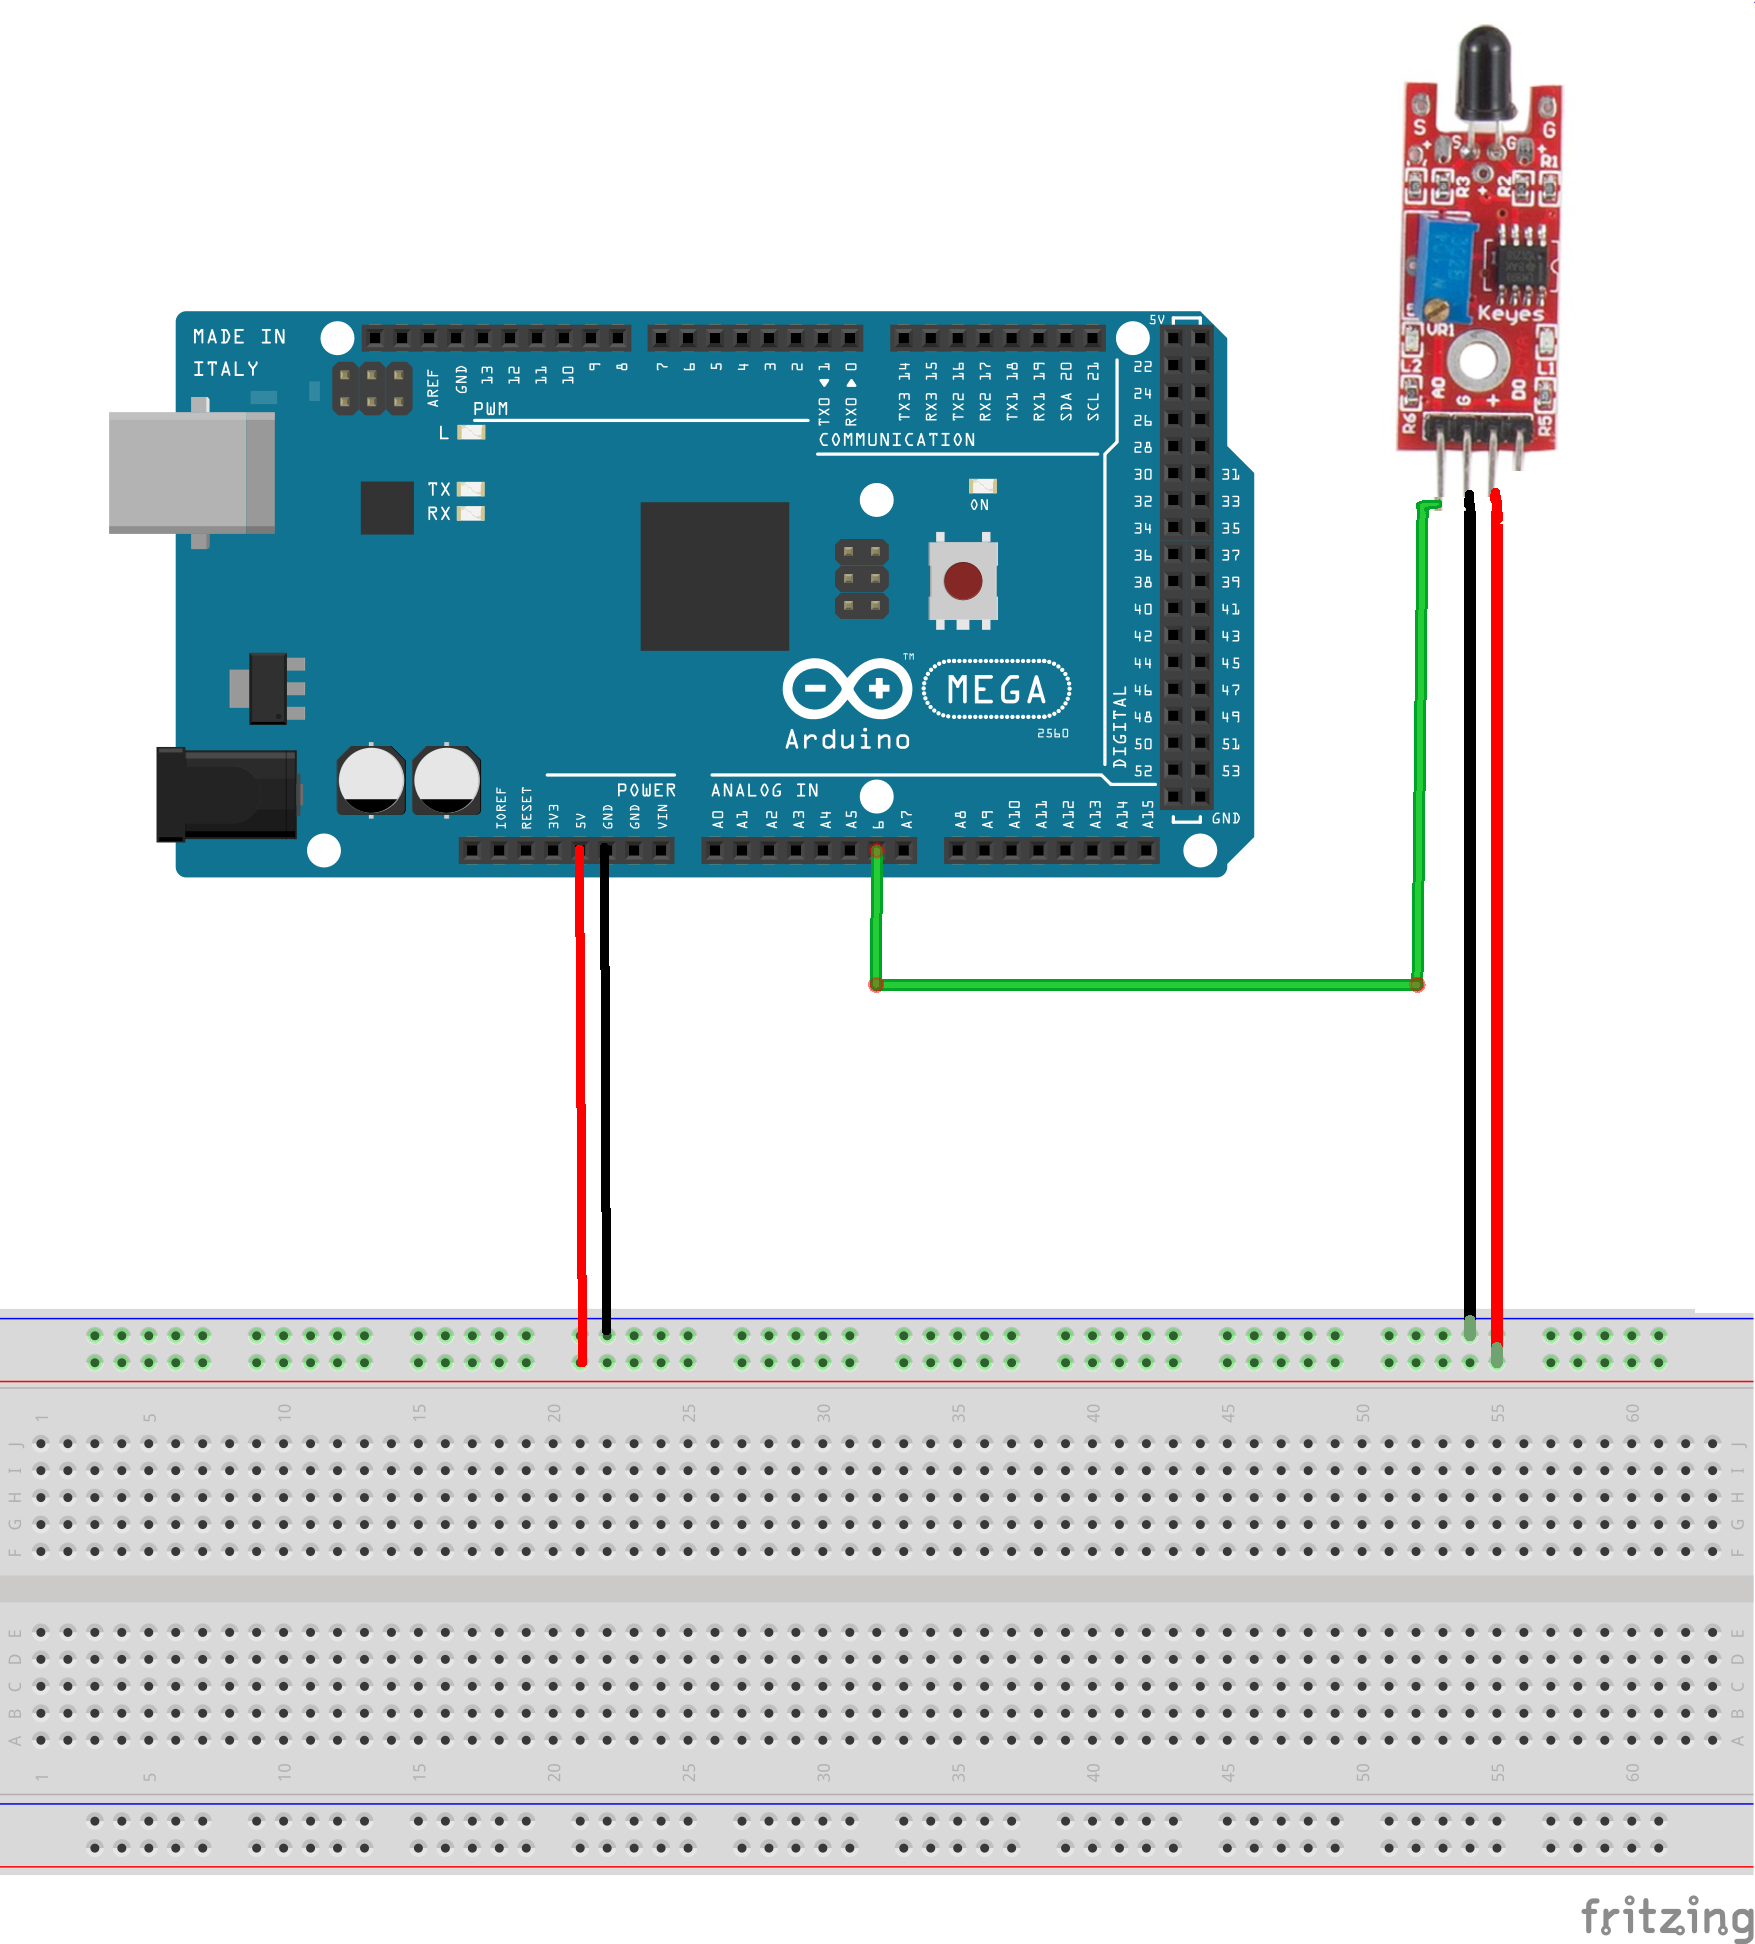
\includegraphics[scale=0.4]{imagenes/llama_conexionado.png}
  \end{center}
  \caption{Vista del conexionado del sensor de llama YG1006.}
  \label{figura:sensor_mq_2_potenciometro}
\end{figure}

 \begin{figure}[H]
  \begin{center}
    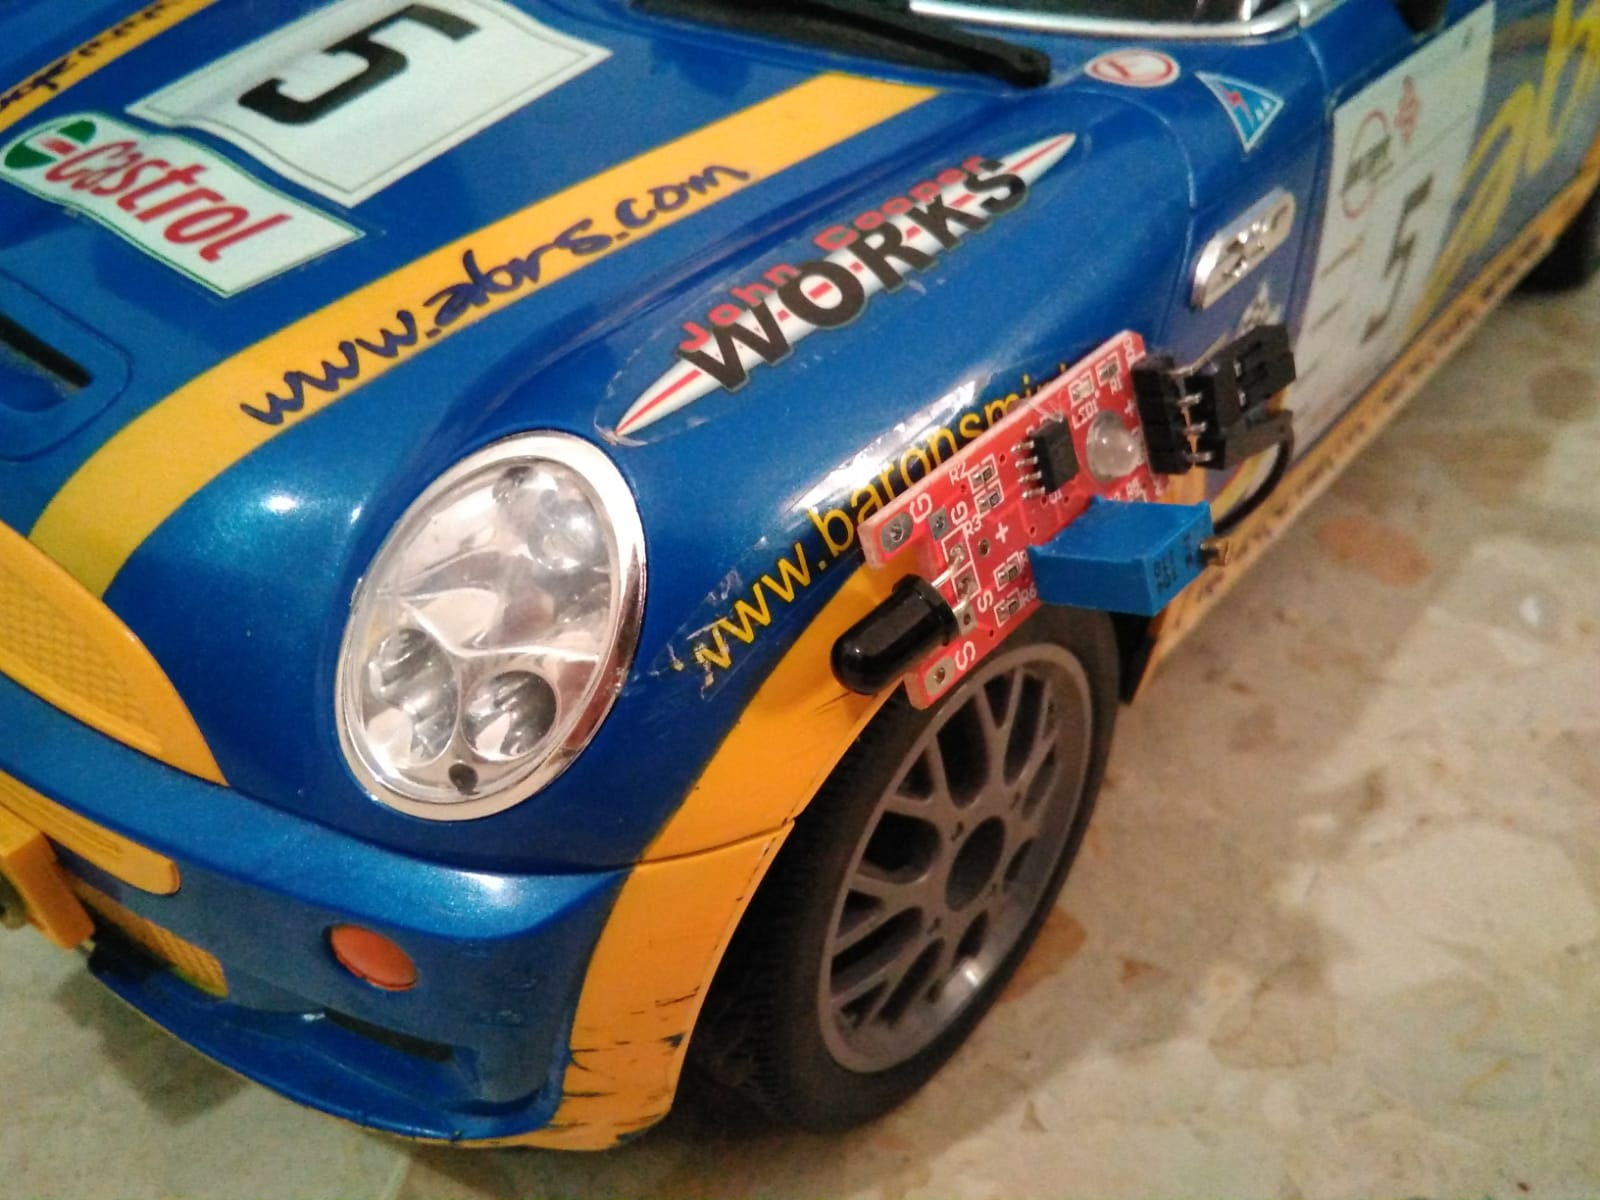
\includegraphics[scale=0.2]{imagenes/robot/llama_instalado.jpeg}
  \end{center}
  \caption{Sensor de llama instalado en la parte delantera del vehículo.}
  \label{figura:sensor_mq_2_potenciometro}
\end{figure}

\subsection{Sensor de proximidad}

La familia de los sensores Sharp GP2Dxx son una gama de sensores muy utilizados tanto en lo que viene a denominarse robótica móvil casera como en el ́ámbito de investigación debido
principalmente a su facilidad de integración y reducido coste (unos 15  Euros). En la Figura \ref{figura:sensor_sharp} puede verse una imagen de un GP2D12.\\

 \begin{figure}[H]
  \begin{center}
    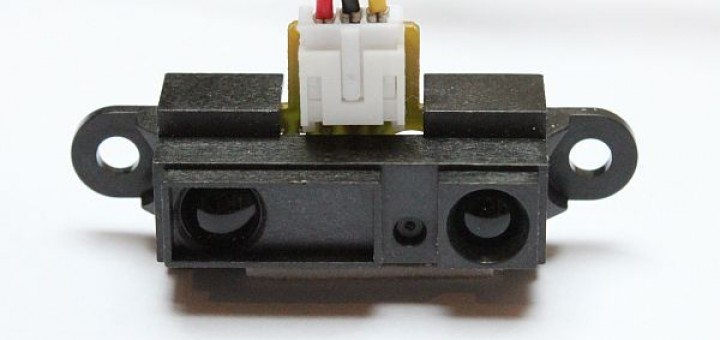
\includegraphics[scale=0.3]{imagenes/sharp.jpg}
  \end{center}
  \caption{Sensor GP2D12.}
  \label{figura:sensor_sharp}
\end{figure}

Los sensores GP2D12 proporcionan una salida analógica entre 0 y 3 voltios dependiendo de la distancia a la que se encuentre el objeto. Dicha salida analógica no es
lineal sino que sigue una curva, la cual se muestra en la figura \ref{figura:curva_sharp}.

 \begin{figure}[H]
  \begin{center}
    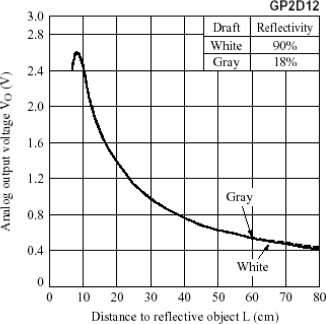
\includegraphics[scale=1.4]{imagenes/curva_sharp.png}
  \end{center}
  \caption{Curva de tensión de salida según la distancia al obstáculo.}
  \label{figura:curva_sharp}
\end{figure}

Estos sensores se basan en el principio de triangulación para realización de las medidas. El elemento situado a la izquierda del sensor según vemos en la figura \ref{figura:sensor_sharp}
es un led infrarrojo que emite un haz que ser ́a rebotado por el objeto y posteriormente recogido por el elemento situado a la derecha. Este ́ultimo se conoce como PSD (Position 
Sensing Device, Dispositivo de Percepción de Posición)  y  puede  entenderse  como  una  lente situada sobre un array de células sensibles a la luz infrarroja. Dependiendo del 
ángulo de incidencia del haz rebotado en la lente, se activa una u otra célula del array permitiendo estimar la distancia a la que se encuentra el objeto.\\

El conexionado del GP2D12 con un microcontrolador requiere de una entrada del conversor analógico-digital a la que se conectará el pin de salida del sensor 
(el de más a la izquierda visto de frente según se muestra en la figura \ref{figura:pines_sharp}). Los otros dos pines corresponden, respectivamente, con \textbf{GND} y con
\textbf{Vcc}, la tensión de alimentación, que deberá ser de 5 voltios.\\

 \begin{figure}[H]
  \begin{center}
    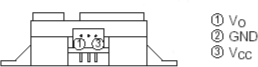
\includegraphics[scale=1.5]{imagenes/pines_sharp.png}
  \end{center}
  \caption{Conexiones del GP2D12.}
  \label{figura:pines_sharp}
\end{figure}

En la siguiente tabla se recoge un resumen de las especificaciones del sensor:\\


\begin{table}[H]
  \begin{center}
    \begin{tabular}{|p{8cm}|p{2cm}|}
      \hline
      {Rango} & {18-80 cm}\\
      {Periodo de lectura} & {40 ms}\\
      {Máximo ángulo de reflexión} & {> 40 $^{\circ}$}\\
      {Tensión de alimentación} & {4.5-5.5 V}\\
      {Ruido de salida} & { < 200 mV }\\
      {Consumo medio} & { 35 mA }\\
      {Consumo de pico} & { 200 mA }\\
      \hline
      \end{tabular}
  \end{center}
  \caption{Resumen de las especificaciones del GP2D12.}
\end{table}

\subsubsection{Conexionado}

El esquema eléctrico es muy simple. Debemos alimentar el módulo conectando GND y
VCC a los pines correspondientes de Arduino y salida D0 a una de las entradas digitales
de Arduino.\\

 \begin{figure}[H]
  \begin{center}
    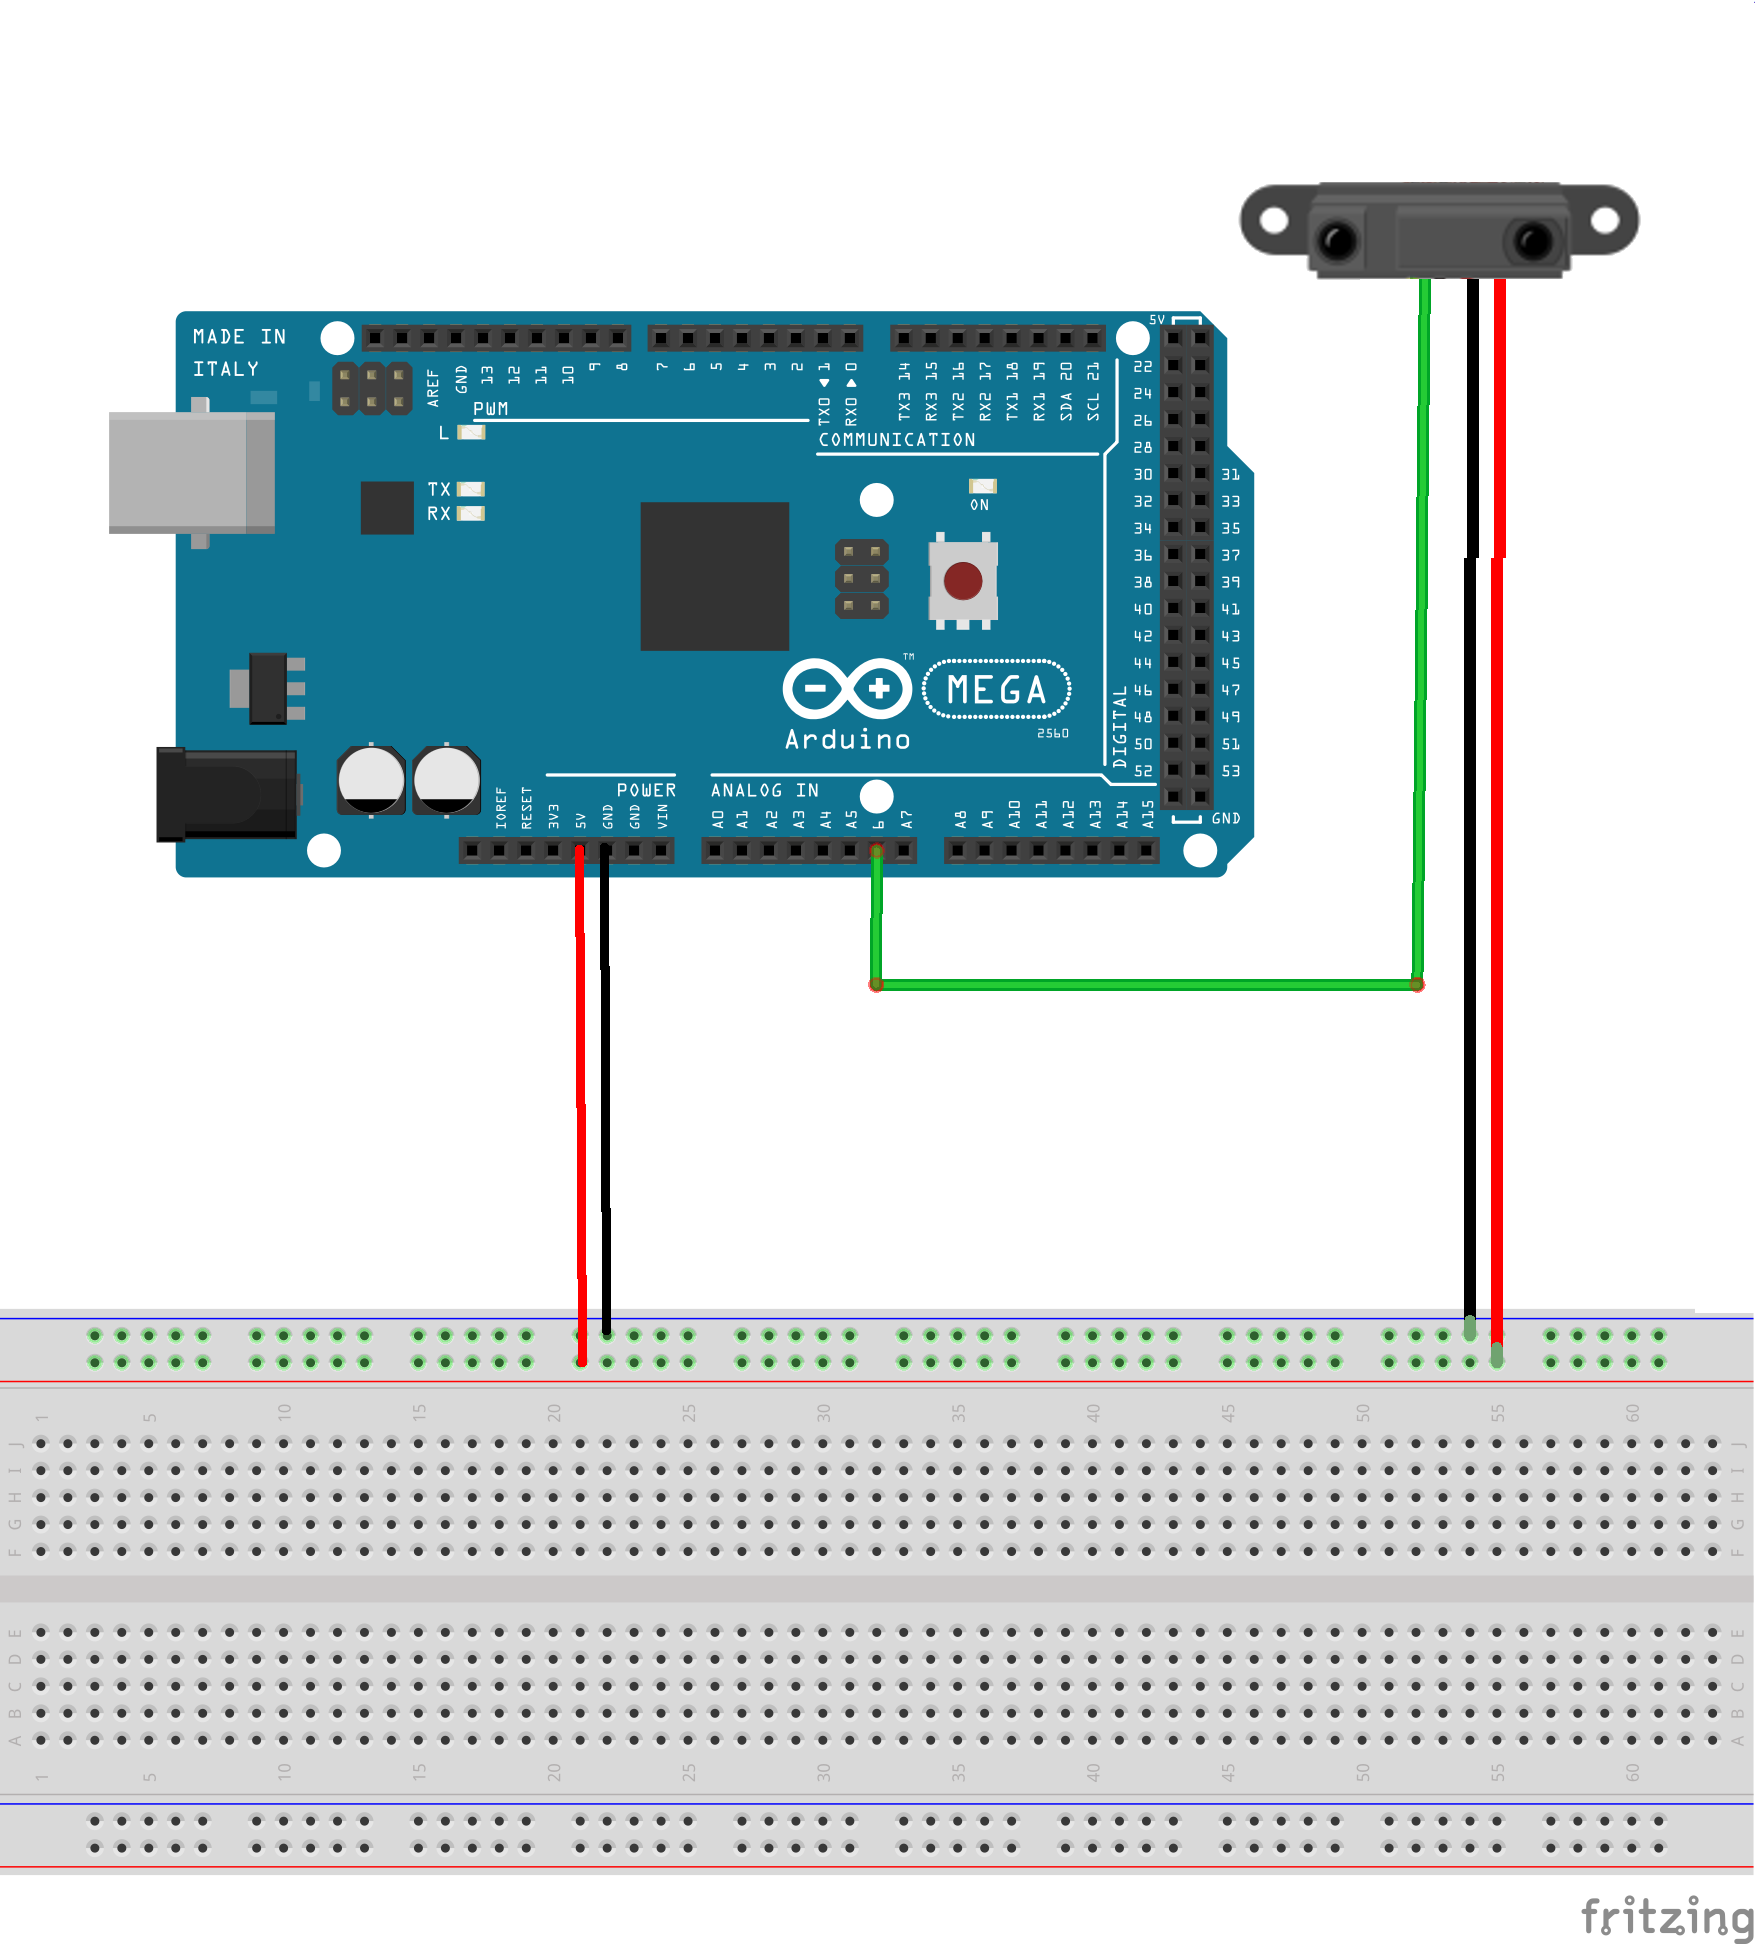
\includegraphics[scale=0.6]{imagenes/sharp_conexionado.png}
  \end{center}
  \caption{Conexionado del GP2D12.}
  \label{figura:pines_sharp}
\end{figure}


 \begin{figure}[H]
  \begin{center}
    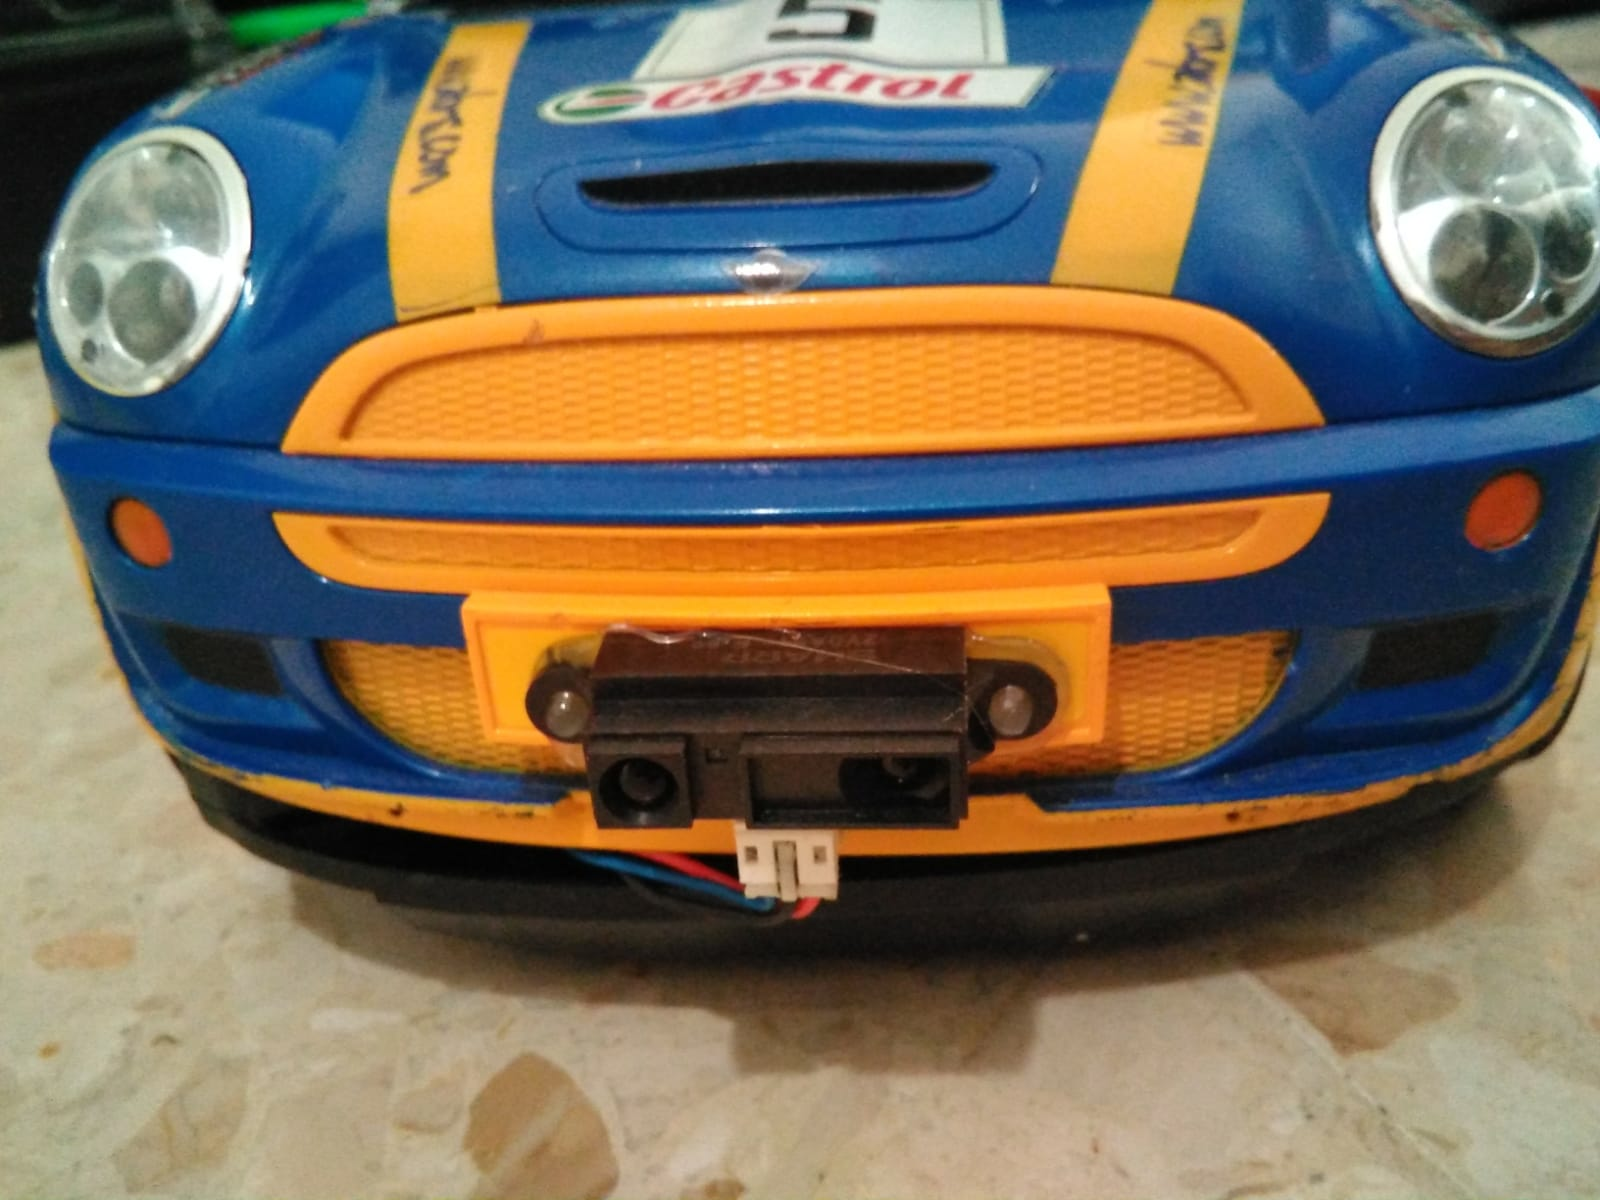
\includegraphics[scale=0.2]{imagenes/robot/sharp_instalado.jpeg}
  \end{center}
  \caption{Sensor de proximidad Sharp GP2D12 instalado en la parte frontal del vehículo.}
  \label{figura:sensor_mq_2_potenciometro}
\end{figure}


\subsection{Buzzer o zumbador}

Un buzzer pasivo, un zumbador o altavoz, son dispositivos que permiten convertir una señal eléctrica en una onda de sonido. Son unos dispositivos muy simples ya que no disponen 
de electrónica interna, por lo que tan solo debemos proporcionar una señal eléctrica para conseguir el sonido deseado.\\

Por contra, los buzzer activos disponen de un oscilador interno siendo exclusivamente necesario alimentarlos para que se emita un sonido.\\

Los buzzer pasivos, como el incorporado en el presente trabajo, tienen la particularidad de que al proporcionar y controlar nosotros la señal eléctrica, poseen la ventaja de
que podemos variar el tono emitido modificando la señal que aplicamos al pin de control permitiendo la generación de melodías.\\

En el caso que compete a este proyecto se ha empleado un buzzer para la emisión de sonidos intermitentes a modo de alarma activados tras la detección de alguna situación de riesgo.
Estas situaciones son determinadas por parte de alguno de los demás sensores de los que dispone el vehículo, como por ejemplo
puede ser la detección de llamas cercanas o ante la presencia de gases peligrosos.\\


Tanto los buzzers como los altavoces son elementos denominados transductores electroacústicos, es decir, son dispositivos que poseen la propiedad de convertir señales eléctricas
en sonido, que para el caso concreto de los buzzers entran en la categoría de los transductores piezoeléctricos. Esto significa que tienen la propiedad de variar su volumen al 
ser atravesados por corrientes eléctricas aprovechando este fenómeno para hacer vibrar una membrana al atravesarlo con una señal eléctrica y con la consecuente emisión del sonido.\\

 \begin{figure}[H]
  \begin{center}
    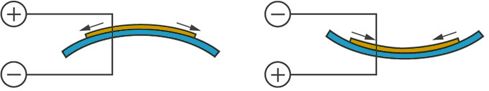
\includegraphics[scale=0.6]{imagenes/diagrama_buzzer.png}
  \end{center}
  \caption{Representación de la variación de volumen del material piezoeléctrico al paso de la corriente.}
  \label{figura:sensor_mq_2_potenciometro}
\end{figure}


\subsubsection{Conexionado}

La conexión con Arduino como en la mayoría de los casos resulta bastante sencilla. Simplemente alimentamos el módulo conectando \textbf{Vcc} y \textbf{GND} a Arduino, y la entrada
de señal conectada a cualquier pin digital de Arduino configurado como salida.\\

 \begin{figure}[H]
  \begin{center}
    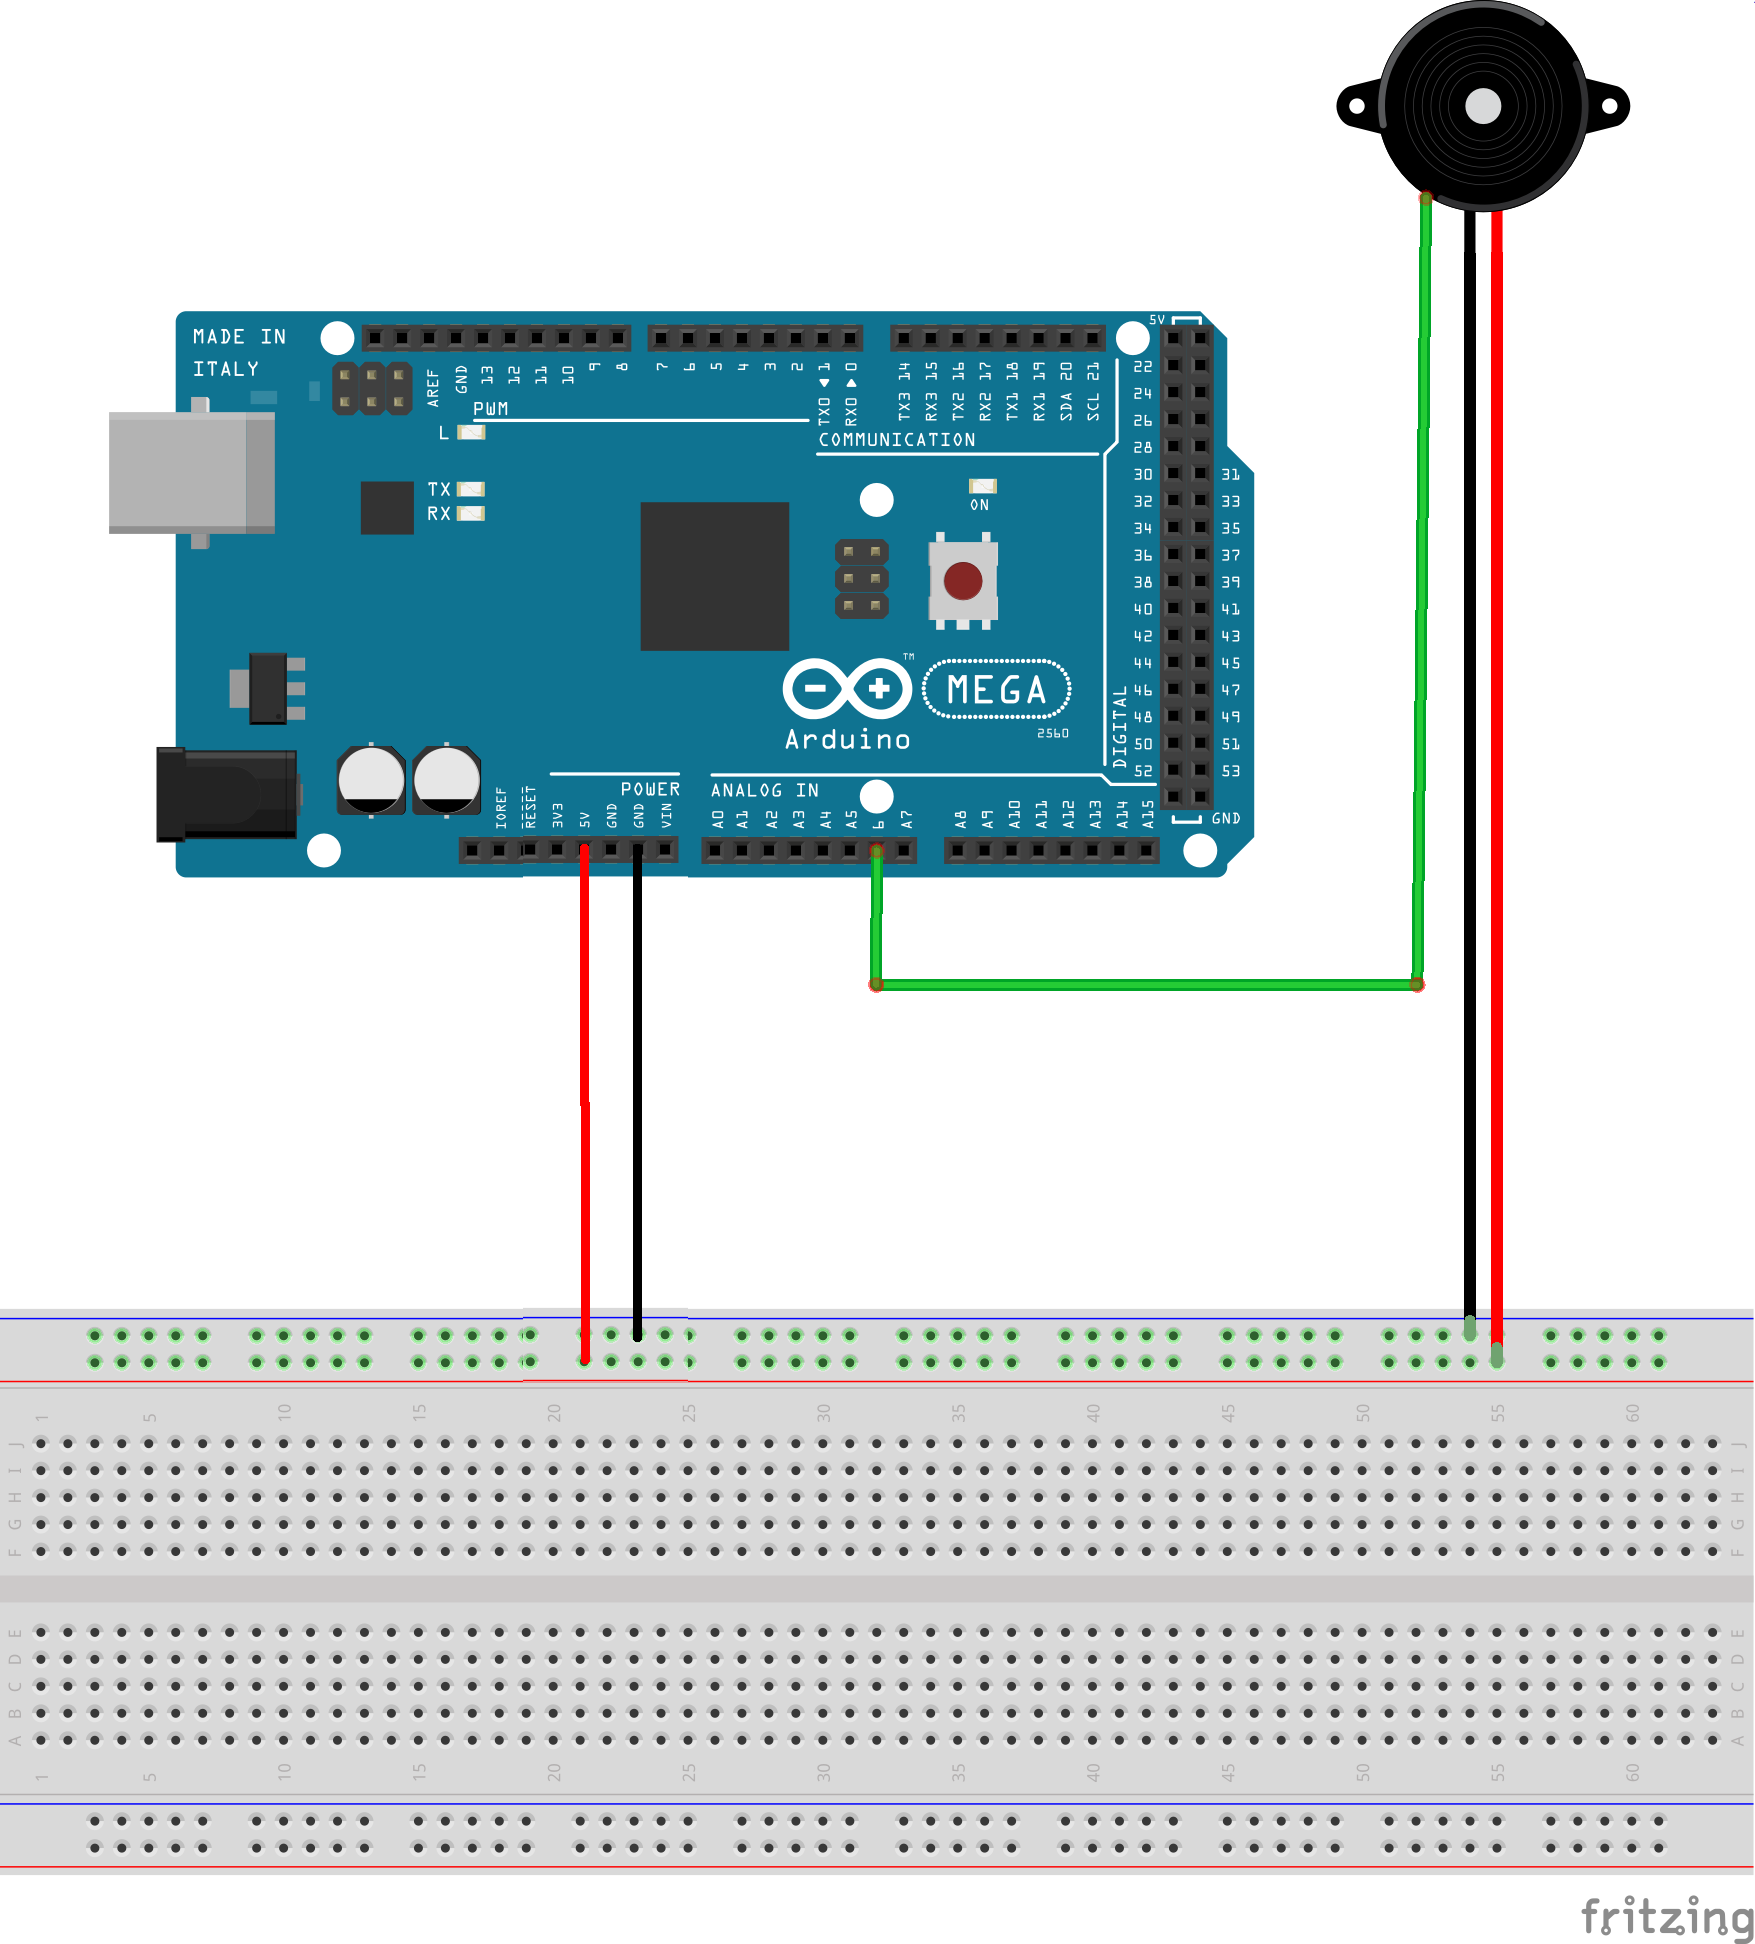
\includegraphics[scale=0.6]{imagenes/conexionado_buzzer.png}
  \end{center}
  \caption{Conexionado del buzzer.}
  \label{figura:pines_sharp}
\end{figure}
